\documentclass{report}
\usepackage[utf8]{inputenc}
\usepackage{mathrsfs}
\usepackage{caption}

\usepackage{graphicx} % Required for inserting images
\usepackage[a4paper,top=2cm,bottom=2.5cm,left=2.5cm,right=2.5cm,marginparwidth=0cm]{geometry}

%link in latex
\usepackage[hidelinks]{hyperref}
\hypersetup{
    colorlinks=false,
    linkcolor=blue,
    filecolor=magenta,      
    urlcolor=cyan,
    pdftitle={Fondamenti_di_elettronica_digitale_BERARDO_CRISTIANO},
    pdfpagemode=FullScreen,
    }
\urlstyle{same}
\usepackage{afterpage}
\usepackage[T1]{fontenc} % codifica dei font
\usepackage[utf8]{inputenc} % lettere accentate da tastiera
\usepackage[italian]{babel} % lingua del documento
\usepackage{url} 
\usepackage{quoting}
\usepackage{xspace}% per lo spazio intelligente
\usepackage{titlesec} % per formato custom dei titoli dei capitoli
\usepackage{tcolorbox}%per i box

\usepackage{float}
\usepackage{sidecap}
\usepackage{amsmath}
\usepackage{pgfplots}   % per i grafici
\pgfplotsset{width=7cm,compat=1.9}
\usepackage{booktabs}
\usepackage{amssymb}

\usepackage{circuitikz}

\usepackage{wrapfig}

\graphicspath{{img/}}

\newcommand{\vds}{V_{DS}}
\newcommand{\vgs}{V_{GS}}
\newcommand{\vt}{V_{T}}
\newcommand{\vtn}{V_{TN}}
\newcommand{\vdd}{V_{DD}}
\newcommand{\vi}{$v_{I}$}
\newcommand{\vo}{$v_{o}$}
\newcommand{\vp}{$V_{+}$}
\newcommand{\vm}{$V_{-}$}

\newcommand{\vil}{$V_{IL}$}
\newcommand{\vih}{$V_{IH}$}
\newcommand{\vol}{$V_{OL}$}
\newcommand{\voh}{$V_{OH}$}
\newcommand{\vl}{$V_{L}$}
\newcommand{\vh}{$V_{H}$}


\newcommand\blankpage{%
    \null
    \thispagestyle{empty}%
    \addtocounter{page}{-1}%
    \newpage}

\begin{document}

\pagestyle{plain}

\thispagestyle{empty}

\begin{center}
  \begin{figure}[h!]
  \centering
    
\includegraphics[trim= 1cm 3.5cm 8.1cm 24.2cm, clip]{img/unitnlogo.pdf}
  \end{figure}

  \vspace{2 cm} 

  \LARGE{Dipartimento di Ingegneria e Scienza dell’Informazione\\}

  \vspace{1 cm} 
  \Large{Corso di Laurea in\\
    %Informatica
    Ingegneria Informatica, delle Comunicazioni ed Elettronica
    %Ingegneria dell'Informazione e Organizzazione d'Impresa
    %Ingegneria Elettronica e delle Telecomunicazioni
  }

  \vspace{2 cm} 
  %\Large\textsc{Manuale di Fisica I\\} 
  %\vspace{1 cm} 
  \Huge\textsc{Fondamenti di Elettronica Digitale\\}
  %\Large{\it{Con un approccio da studente a studente}}


  \vspace{2 cm} 
  \begin{tabular*}{\textwidth}{ c @{\extracolsep{\fill}} c }
  \Large{Docente} & \Large{Studente}\\
  \Large{Roberto Passerone}& \Large{Cristiano Berardo 234428}\\
  \end{tabular*}

  \vspace{2 cm} 

  \Large{Anno accademico 2023/2024}
  
\end{center}
\afterpage{\blankpage}


\tableofcontents


\clearpage

 \chapter{Il Silicio}

\section{Materiali}
\begin{quote}
    Per approcciare alla materia servirebbe studiare la meccanica quantistica
\end{quote}

I materiali possono essere di tre tipologie;
\begin{itemize}
    \item Isolanti;
    \item Conduttori;
    \item Semiconduttori.
\end{itemize}

Tutti si distinguono per la loro resistività, vedremo in modo particolare i \textbf{semiconduttori}, ottenuti dalla colonna IV, oppure dalla combinazione della colonna III e V della tavola periodica.

%da inserire la tabella


\begin{figure}[htbp]
    \begin{minipage}[htbp]{0.5\textwidth}
        \centering
        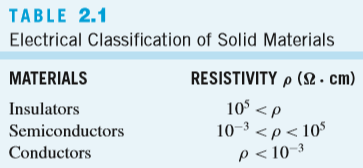
\includegraphics[width=0.8\linewidth]{img/ECSM.png}
        \caption{Eletrical Classification of Solid Materials} 
    \end{minipage}
    \begin{minipage}[htbp]{0.5\textwidth}
    \centering

    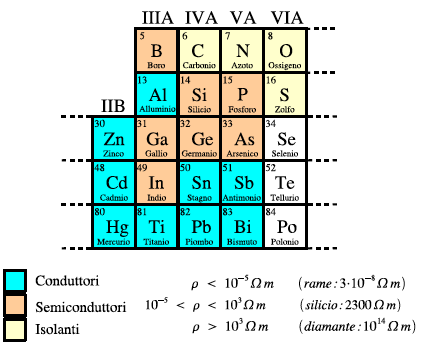
\includegraphics[width=0.8\linewidth]{img/TavolaPeriodica.png}    

    
    \end{minipage}
\end{figure}



% \begin{figure}[htbp]
%     \centering
%     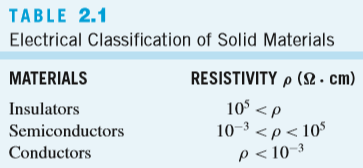
\includegraphics[width=0.4\linewidth]{img/ECSM.png}
%     \caption{Eletrical Classification of Solid Materials}    
% \end{figure}

% \begin{figure}[htbp]
%     \centering
%     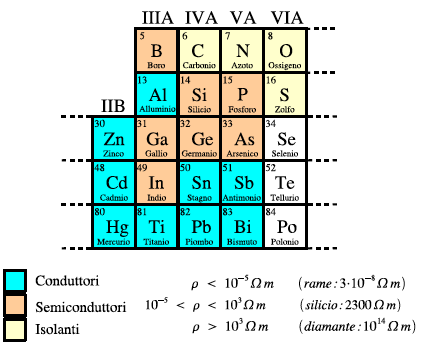
\includegraphics[width=0.55\linewidth]{img/TavolaPeriodica.png}    
% \end{figure}

\paragraph{Esempio:} Prendiamo un filo lungo 1 cm, area $10\mu m \cdot 10\mu m$. $L/A = 1/0.001\cdot0.001 = 10^6$

Prendendo come resistività $\rho = 10^5$ e poi $\rho = 10^{-3}$ ed utilizzando la relazione $\rho = R \frac{A}{L}$, otteniamo dei valori di resistenza di diversi ordini di grandezza differenti: $R = 100\,G\Omega \hspace{0.5cm} 1K\Omega$.

\newpage
\subsection{Struttura cristallina del silicio}
\begin{figure}[htbp]
    \centering
    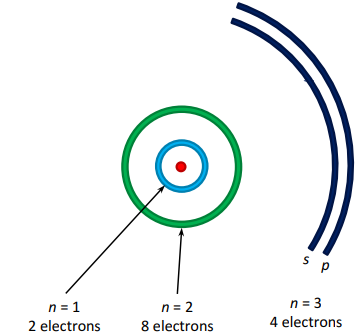
\includegraphics[width=0.35\linewidth]{img/silicio.png}
    \caption{Atomo di silicio}
    
\end{figure}

Alla temperatura dello zero assoluto, $0^{\circ}\,K = -273.15^{\circ}\,C$, tutti gli elettroni sono fissi in un legame covalente e dunque il materiale risulta isolante. Questo dovuto al fatto che nessuna carica, elettrone, si può muovere.

A temperature più alte, fornendo quindi dell'energia, alcuni legami si rompono e l'elettrone, sull'orbitale più esterno, è libero per la conduzione.


\begin{figure}[htbp]
    \centering
    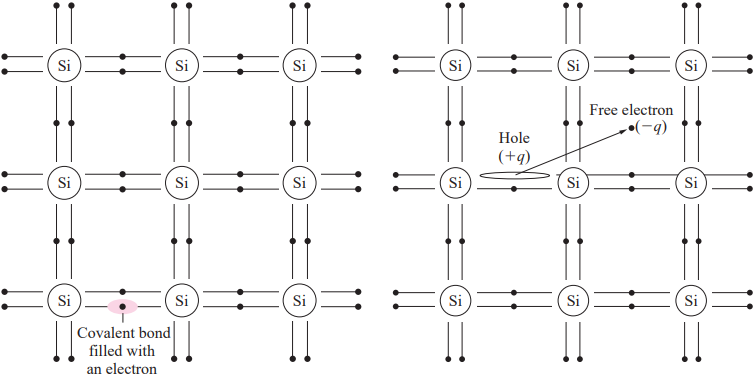
\includegraphics[width=0.8\linewidth]{img/legameSilicio.png}
    \caption{Struttura cristallina Silicio}    
\end{figure}


A questo punto si vede anche in figura che un elettrone che si stacca da un legame covalente lascia dietro di se un buco chiamato \textbf{hole} o \textbf{lacuna} che dovrà essere riempito.

\subsection{Densità di elettroni liberi}
Il numero di elettroni liberi in dipende da due fattori:
\begin{itemize}
    \item Temperatura;
    \item Materiale;
\end{itemize}


Utilizzando la seguente formula si possono trovare la densità di cariche:

\begin{equation}
    n_i^2 = BT^3\exp -\frac{E_G}{kT} 
\end{equation}

dove:
\newpage
\begin{itemize}
    \item $n_i = $ concentrazione di elettroni per $cm^3$
    \item $E_G = $ semiconductor bandgapenergy [$eV$] (elettronvolt, energia minima per rompere un legame)
    \item $k = $ costante di Boltzmann equivalente a $8.62 10^{-5}\,\,\,[eV/K]$
    \item $T = $ temperatura, [$K$]
    \item $B =$ parametro del materiale, $1.08 10^{31}\,\,\,[K^{-3}cm^{-6}] $ per il Si
\end{itemize}

\begin{figure}[htbp]
    \centering
    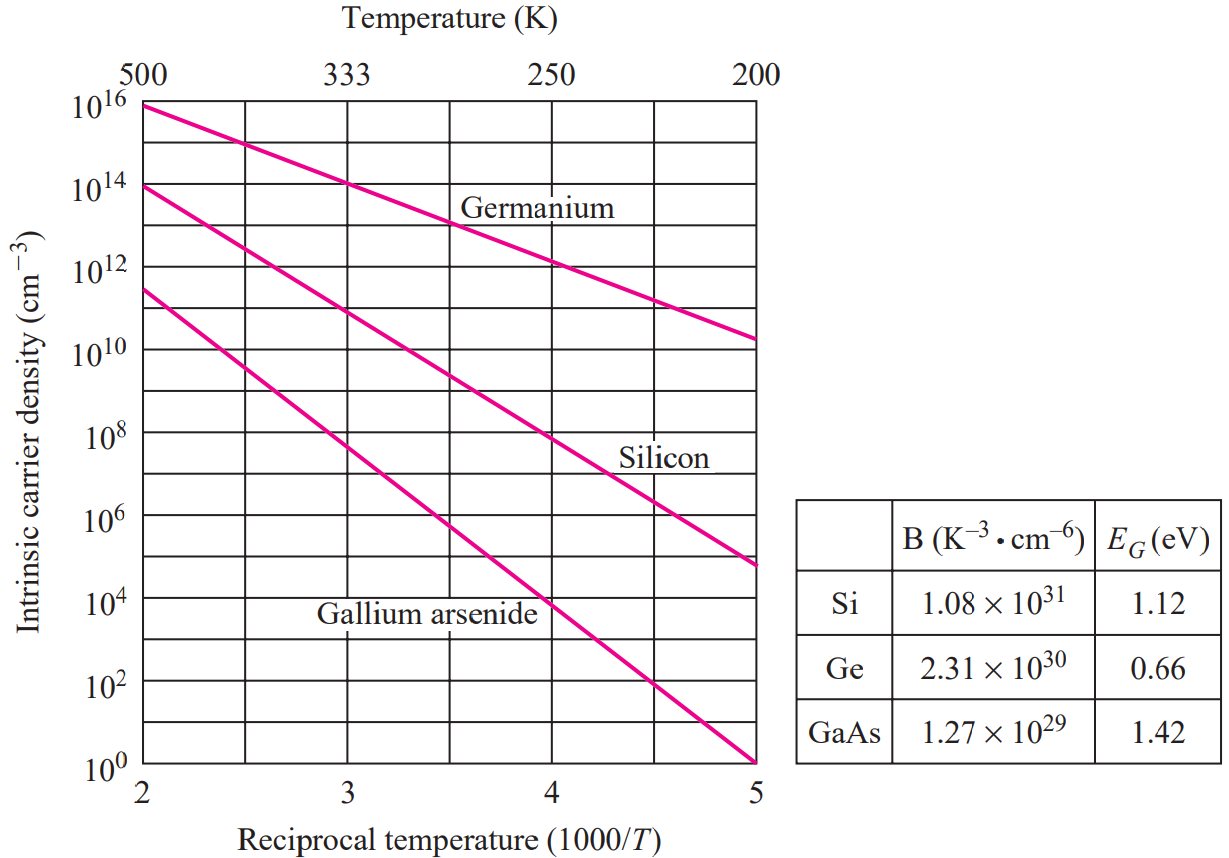
\includegraphics[width=0.75\linewidth]{img/bandGap.png} 
\end{figure}

\paragraph{Calcoliamo le cariche nel silicio:}

Sappiamo che la densità del silicio è: $5 10^{22} /cm^{3}$, applicando la formula a temperatura ambiente otteniamo:

\begin{equation*}
    n_i = 6.73 10^9 \approx 10^{10} /cm^3
\end{equation*}

\paragraph{Lacune: }
Un elettrone libero lascia dietro di se un buco, il quale dovrà essere riempito. Un elettrone da un altro legame può riempire il buco, che si sposta dalla parte opposta all'elettrone.

La lacuna la possiamo considerare come una carica \textbf{positiva}.
\paragraph{}
All'equilibrio, la densità di elettroni liberi e di lacune è identica.

\begin{equation*}
    n = n_1 = p \quad pn = n_i^2
\end{equation*}

dove 
\begin{itemize}
    \item n = concentrazione di elettroni liberi al $cm^3$;
    \item $n_1$ = numero di elettroni al $cm^3$, densità di e al$cm^3$;
    \item p = concentrazione di lacune libere al $cm^3$;
\end{itemize}

\begin{figure}[htbp]
    \centering
    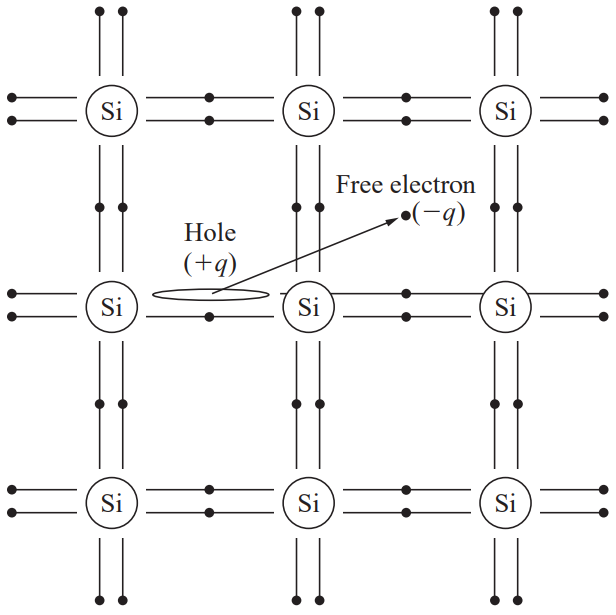
\includegraphics[width=0.4\linewidth]{img/hole.png}
    \caption{Spostamento di lacuna}    
\end{figure}

\newpage
\section{Corrente di drift}
Una elettrone libero, che rappresenta dunque una carica, può generare una corrente elettrica.

La corrente rappresenta la quantità \textbf{netta} di cariche per unità di tempo che attraversano la selezione del materiale. Il valore della corrente dipende dalla \textbf{velocità}. All'equilibrio termico, le cariche si muovono caoticamente e casualmente in tutte le direzioni, cambiando direzione ad ogni urto con un atomo del cristallo.

Questo fa si che:
\begin{itemize}
    \item La velocità media sia \textbf{nulla};
    \item La corrente totale risulti essere \textbf{zero}
\end{itemize}

\begin{figure}[htbp]
    \centering
    
\includegraphics[width=0.14\linewidth]{img/moto-Casuale.png}    
\end{figure}


Applicando un \textbf{campo elettrico} E, le cariche tendono a muoversi nella sua direzione (drift).

\begin{itemize}
    \item Legge	di	Coulomb:\quad$\vec{F} = q\vec{E}$;
    \item Seconda	legge	di	Newton: \quad $\vec{F} = m\vec{a}$
    \item Quindi: $\vec{a} = \frac{q}{m}\vec{E}$
\end{itemize}

L'effetto della struttura dei materiali, essendoci gli atomi, fa si che le collisioni avvengano e modifichino la traiettoria dell'elettrone. Questo scontro fa perdere energia agli elettroni, effetto Jule, e l'effetto totale è quello di godere di un moto costante verso una direzione.

\begin{figure}[htbp]
    \centering
    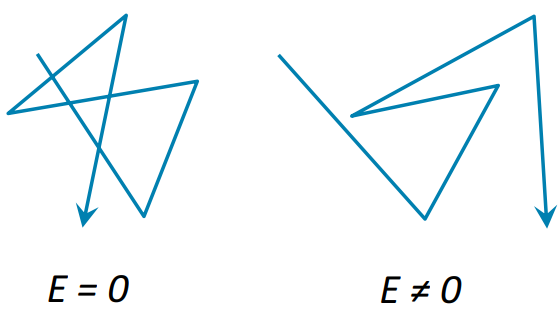
\includegraphics[width=0.33\linewidth]{img/campo_elettromagentico.png}  
\end{figure}

\newpage
La velocità risulta essere proporzionale al campo elettrico:

\begin{equation}
    v_n = -\mu_n\vec{E} \quad\quad v_p = \mu_p\vec{E}
\end{equation}

dove 
\begin{itemize}
    \item $v_n$ = Velocità elettroni
    \item $\mu_n$ = mobilità	degli	elettroni,	$1350\, cm^2/V\cdot s$	in	Si	intrinseco (puro).
    \item $v_p$ = Velocità lacune
    \item $\mu_p$ = mobilità	degli	elettroni,	$500\, cm^2/V \cdot s$	in	Si	intrinseco (puro).
\end{itemize}

Le	\textbf{lacune}	hanno	\textbf{minore	mobilità}	perché	costrette	a	muoversi	
nella	struttura,	mentre	gli	elettroni	godono di maggiore libertà.

\subsection{Velocità	di	saturazione}
Come visto prima, la velocità delle cariche risulta essere proporzionale, in media, al campo elettrico. Questo è vero fino ad un certo valore perché anche le cariche non possono superare la velocità	della luce, $300\,000\,\,\,[Km/s]$.

\paragraph{}
Dunque esiste un limite di saturazione il quale limita la risposta in frequenza e dunque anche la velocità di una porta logica (clock limitato).

\begin{figure}[htbp]
    \centering
    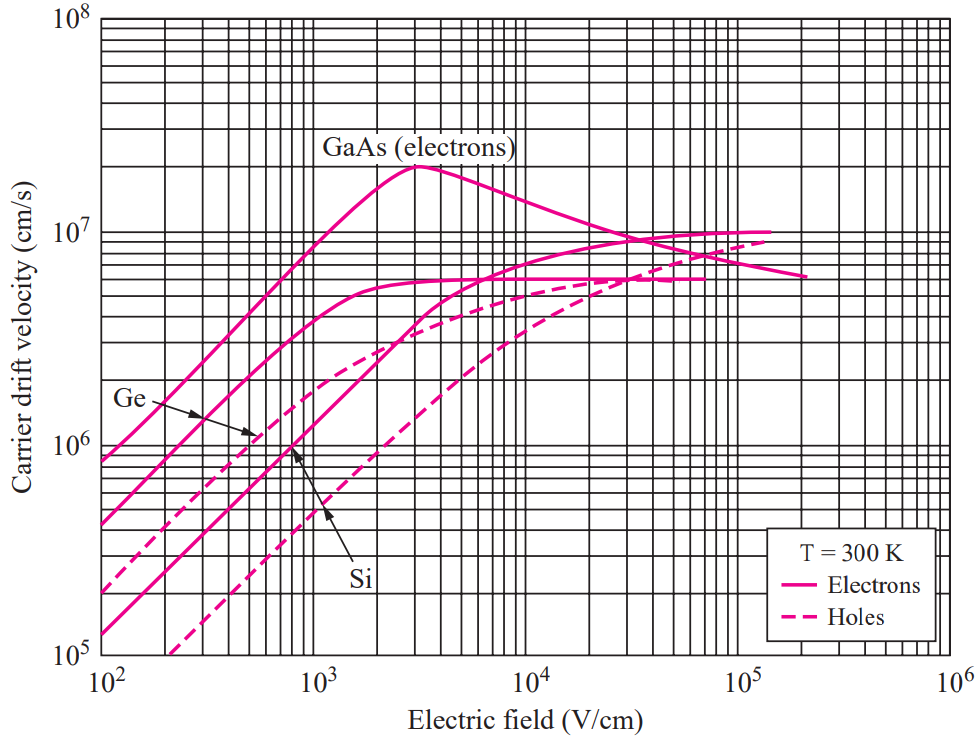
\includegraphics[width=0.75\linewidth]{img/saturazione.png}
    \caption{Velocità	di	saturazione}
\end{figure}

\newpage
\subsection{Calcolo della corrente di drift}
Valutiamo	la	carica	che	attraversa	una	superficie	nell'unità	di	tempo.


\begin{figure}[htbp]
    \centering
    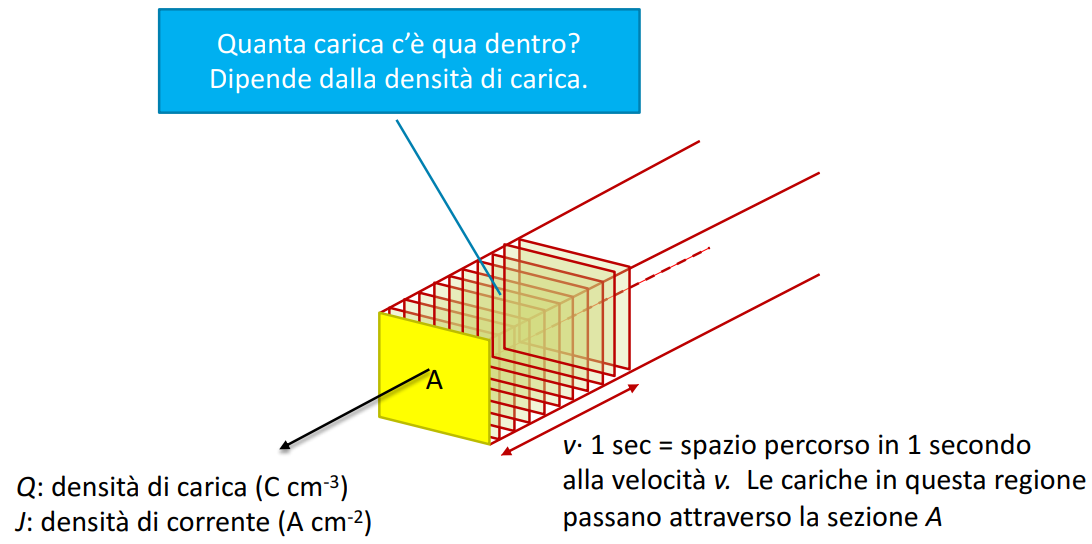
\includegraphics[width=0.9\linewidth]{img/carica_drift.png}
    \caption{Corrente di Drift}    
\end{figure}

Ricordiamo le seguenti formule:

\begin{equation*}
    I = JA = \sigma \frac{A}{L}\vec{E}L = GV \quad\quad q = 1.6\cdot10^{-19}
\end{equation*}
\begin{equation}
    j_n^{drift} = Q_nv_n = (-qn)(-\mu_n\vec{E}) = qn\mu_n\vec{E} \qquad[A/cm^2]
\end{equation}
\begin{equation}
    j_p^{drift} = Q_pv_p = (-qp)(-\mu_p\vec{E}) = qp\mu_n\vec{E} \qquad[A/cm^2]
\end{equation}
\begin{equation}
    j_T^{drift} = j_n^{drift} + j_p^{drift}Q_pv_p = q(n\mu_n + p\mu_p)\vec{E} = \sigma \vec{E}
\end{equation}

$\sigma: q(n\mu_n + p\mu_p)$ rappresenta la conduttività.

\paragraph{A temperatura ambiente}

\begin{itemize}
    \item[] $n = n_i = p = 10^{10}$
    \item[] $\sigma = (1.6*10^{-19})10^{10}(1350+500) = 2.96*10^{-6}$
\end{itemize}
\begin{equation*}
    j_T^{drift} = j_n^{drift} + j_p^{drift}Q_pv_p = q(n\mu_n + p\mu_p)\vec{E} = \sigma \vec{E}
\end{equation*}
\begin{equation*}
    \rho = \frac{1}{\sigma} = 3.38*10^{5}\, \omega cm
\end{equation*}

Dunque il silicio a temperatura ambiente rientra nella famiglia degli \textbf{isolanti}.

\paragraph{Conduttore in rame lungo 1m, di diametro 1mm e tensione di 1V}

\begin{itemize}
\centering
    \item[]  $R = \rho\frac{L}{A} = 1.68 10^{-8} \frac{1}{\pi 0.0005^2} = 0.0214 \,\omega$
    \item[]  $I = \frac{V}{R} = \frac{1}{0.0214} = 46.7\,A$
    \item [] $J = \frac{I}{A} = \frac{46.7}{\pi 0.0005^2 } = 59 10^6\,Am^{-2}$
    \item[]  $v = \frac{J}{nq} = \frac{59 10^6}{8.46 10^{28} 1.6 10^{-19}} = 0.0044 ms^{-1} = 4.4\,mms^{-1}$ 
\end{itemize}

Questa risulta essere la velocità netta di drift, gli elettroni si muovo a	velocità molto	più elevata,	ma	caoticamente.
Dunque gli elettroni impiegano delle ore per fare quale metro in un filo di rame, come è possibile dunque che la luce di una lampadina di accenda subito? 
\paragraph{}
Questo è dovuto alla \textbf{reazione a  catena} che da al via al tutto, e in generale è il \textbf{campo elettromagnetico} che si sposta rapidamente e che fa muovere gli elettroni.

\section{Impurità}
L'aggiunta	di	impurità	ci	permette	di controllare	la	resistività. 

\subsection{Atomi	pentavalenti }
Contribuiscono con un	elettrone	in	più, alcuni di questi atomi sono nella colonna V della tavola periodica:



\begin{itemize}
    \centering
    \item[] Fosforo, Arsenico, Antimonio
\end{itemize}




Questi atomi, superati i $0^{\circ}\,K$ , si ionizzano più velocemente ed essendo che hanno un elettrone in più, rispetto al Si, questo sarà libero di viaggiare libero nel reticolo cristallino. Essendo che P, As e Sb possono donare cariche, vengono chiamati \textbf{donatori}.

\subsection{Atomi	trivalenti }
Contribuiscono con un	\textbf{elettrone}	in	meno e dunque contribuiscono ad una \textbf{lacuna}, alcuni di questi atomi sono nella colonna III della tavola periodica:
\begin{itemize}
\centering
    \item[] Boro
\end{itemize}

Questi atomi, a differenza di quelli sopracitati, vengono chiamati \textbf{accettori} in quanto avendo sull'orbitale più esterni un elettrone in meno rispetto a Si, formano una lacuna la quale dovrà essere riempita da un elettrone del Si.
\paragraph{}
La conduzione è affidata prevalentemente a elettroni o lacune.

\paragraph{}
\begin{figure}[htbp]
    \centering
    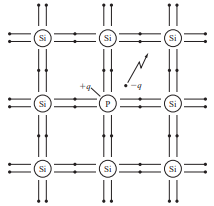
\includegraphics[width=0.35\linewidth]{img/energia_p.png}    
\end{figure}
Poca energia/calore è sufficiente per liberare le cariche, dunque queste impurità modificano la concentrazione di portatori:

\begin{itemize}
    \item $n = p$: Stiamo parlando del silicio senza impurità chiamato \textbf{intrinseco}
    \item $n \neq p$: Pariamo di silicio con aggiunta di impurità chiamato \textbf{estrinseco}
    \begin{itemize}
        \item[] $n > p$, il silicio è di \textbf{tipo n}, ovvero i portatori di maggioranza sono gli \textbf{elettroni}, donatori di ioni positivi. Questo silicio ha una migliore mobilità.
        \item[] $n < p$, il silicio è di \textbf{tipo p}, ovvero i portatori di maggioranza sono le \textbf{lacune}, donatori di ioni negativi. Questo silicio ha una peggiore mobilità.
    \end{itemize}
\end{itemize}
\newpage
\begin{figure}[htbp]
    \centering
    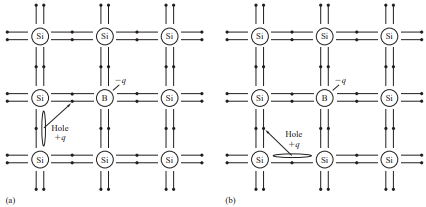
\includegraphics[width=0.75\linewidth]{img/boiro_energia.png}       
\end{figure}

\paragraph{}
Le concentrazioni di impurità sono normalmente dell'ordine di $10^{14}$ fino a $10^{21}$ atomi per $cm^3$, per confronto, la	concentrazione	intrinseca	di	portatori	è	dell'ordine	di	$10^{10}$ cariche	per	$cm^3$.
\paragraph{}
La	concentrazione	dei	portatori	\textbf{maggioritari} è	quindi	praticamente	uguale	alla	concentrazione	di	impurità	ed	è	
praticamente	costante. Sono le \textbf{impurità} che portano il più alto contenuto di elettroni liberi, l'equilibrio termico ne porta molte meno. Infatti aggiungere $10^{14}$ impurità significa aggiungere la stessa quantità di cariche o lacune.

\subsection{Conduzione}
Occorre	calcolare	la	concentrazione	di	portatori. La	carica	totale	del	conduttore	deve	essere	globalmente	nulla.
\begin{itemize}
    \item $N_D$ =	concentrazione	donatori	(ioni	positivi)
    \item $N_A$ =	concentrazione	accettori	(ioni	negativi)
\end{itemize}
\begin{equation*}
    q(N_D + p - N_A - n) = 0
\end{equation*}

Vale ancora la relazione (legge dell'azione di massa): $pn = n^2_i$
\paragraph{}
Quindi per i semiconduttori di tipo n: 
\begin{equation*}
    n^2 - (N_D - N_A)n - n_i^2\qquad n = \frac{(N_D - N_A) + \sqrt{(N_D - N_A)^2 + 4n_i^2}}{2}
\end{equation*}

In pratica se $(N_D - N_A) >> 2n_i$ allora:
\begin{equation*}
    n = N_D - N_A\qquad p = \frac{n_i^2}{n}
\end{equation*}

\subsubsection{Per il silicio di tipo p:}
\begin{equation*}
    p = N_A - N_D\qquad n = \frac{n_i^2}{p}
\end{equation*}

\paragraph{Pertanto:}
La	concentrazione	dei	portatori	\textbf{maggioritari}	è	praticamente	costante e	\textbf{indipendente	dalla	temperatura}.

La	concentrazione	dei	portatori	\textbf{minoritari} è	invece	proporzionale	a	$n_i^2$ e	fortemente \textbf{dipende		dalla	temperatura}

Per	esempio,	drogando	con	Boro	a	$10^{16}/cm^3$  e	con	Fosforo	a	$2\cdot10^{15}/cm^3$ a	temperatura	ambiente:

\begin{equation*}
    N_A = 10^{16} \qquad N_D = 2\cdot10^{15}
\end{equation*}
\begin{equation*}
   p = (N_A - N_D) = 8.00 \cdot 10^{15}
\end{equation*}
\begin{equation*}
   n = \frac{n_i^2}{p} = 1.25 \cdot 10^{4}
\end{equation*}

\paragraph{A 400 Kelvin (126,85°C):}
\begin{equation*}
   n_i^2 = 5.4 \cdot10^{24} \qquad p = (N_A - N_D) = 8.00\cdot10^{15} \qquad n = \frac{n_i^2}{p} = 6.75 \cdot 10^{8}
\end{equation*}


\subsection{Resistività in materiali estrinseci}
Il	drogaggio	riduce	la	mobilità	dei	portatori, infatti un silicio drogato con $N_D = 2\cdot10^{15}/cm^3$

\begin{equation*}
    n = 2\cdot10^{15}/cm^3 \qquad p = 10^{20}/2\cdot10\cdot10^{15} = 5\cdot10^{4}/cm^3
\end{equation*}

Questo silicio di tipo p ha una mobilità inferiore:
\begin{equation*}
    \mu_n = 1320\qquad\mu_p = 460
\end{equation*}

La conduttività e resistività sono:

\begin{equation*}
    \sigma = (1.6\cdot10^{-19})[(2\cdot10^{15})1320 + (5\cdot10^4)460] = 0.422
\end{equation*}

\begin{equation*}
    \rho = 1/\sigma = 2.37\,\,\,[\Omega cm]
\end{equation*}

Il silicio ora è un semiconduttore, da notare che una piccola frazione di impurità ($2\cdot10^{15} \text{ contro } 5\cdot10^{22}$) cambia la resistività di 5 ordini di grandezza, prima era: $3.38\cdot10^{5}$.

Dunque possiamo controllare la resistività del silicio.

\begin{figure}[htbp]
    \centering
    \includegraphics[width=0.65\linewidth]{img/resistività_SI.png}    
\end{figure}

\newpage
\section{Corrente di diffusione}
Se	il	drogaggio	non	è	uniforme	le	concentrazioni	dei	portatori	
variano	lungo	il	cristallo. Si	generano	quindi	correnti	di	diffusione	proporzionali	al	gradiente	di	
concentrazione.

\paragraph{}
I	portatori	vanno	da	regioni	a	maggiore	concentrazione	a	regioni	a minore	concentrazione, proprio come succede con lo scambio termico.
\begin{figure}[htbp]
    \centering
    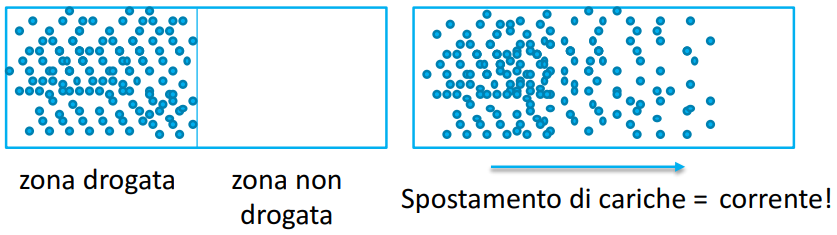
\includegraphics[width=0.7\linewidth]{img/corrente_diff.png}
\end{figure}

Si è notato che questa corrente di diffusione segue le seguenti ugualianze:

\begin{equation*}
    J_p^{diff} = (+q)D_p\biggl(-\frac{\partial p}{\partial x} = -qD_p\frac{\partial p}{\partial x}\biggl)
\end{equation*}
\begin{equation*}
    J_n^{diff} = (-q)D_n\biggl(-\frac{\partial n}{\partial x} = -qD_n\frac{\partial n}{\partial x}\biggl)
\end{equation*}
Dove $D_p \text{ e } D_n$ sono le diffusività	di	lacune	ed	elettroni	che	dipendono	dalla	
mobilità	e	temperatura	secondo	la	relazione	di	Einstein:

\begin{equation*}
    \frac{D_n}{\mu_n} = \frac{kT}{q} = \frac{D_p}{\mu_p} \qquad \text{ dove } V_t = kT/q = 0.0258V \text{ a } 300K
\end{equation*}

\section{Corrente totale}

Per ottenere la corrente totale, applicando un campo elettrico, dobbiamo sommare la corrente di drift e di diffusione:
\begin{equation}
    j_n^T = q\mu_nn\vec{E} + qD_n\frac{\partial n}{\partial x}
\end{equation}
\begin{equation}
    j_p^T = q\mu_pp\vec{E} + qD_p\frac{\partial p}{\partial x}
\end{equation}

Oppure applicando la relazione di Einstein: 
\begin{equation}
    j_n^T = q\mu_nn\biggl(\vec{E} + V_T\frac{1}{n}\frac{\partial n}{\partial x}\biggl)
\end{equation}
\begin{equation}
    j_p^T = q\mu_pp\biggl(\vec{E} - V_T\frac{1}{p}\frac{\partial p}{\partial x}\biggl)
    \label{eq_eine}
\end{equation}

Per completare il sistema dobbiamo considerare	la	dipendenza	del	campo	dalla	carica:

\begin{equation*}
    \nabla \cdot \varepsilon \vec{E} = Q
\end{equation*}

Dove $\varepsilon$ è la permittività e Q la	densità	di	carica	nello	spazio.

\newpage
\section{Take away}
Tramite	il	drogaggio	possiamo	controllare	la	
concentrazione	delle	cariche	nel	silicio, cariche	costituite	da	\textbf{elettroni}	e/o	\textbf{lacune}.
\paragraph{}
La corrente si può dividere in due componenti:
\begin{itemize}
    \item Corrente	di	\textbf{drift} dovuta	ad	un	campo	elettrico	applicato;
    \item Corrente	di	\textbf{diffusione} dovuta	a	gradienti	di	concentrazione.
\end{itemize}

I	dispositivi	elettronici	sono	realizzati	tramite	aree	di	tipo	
p	ed	n	collegate.

\section{Processo costruttivo}
I	circuiti	sono/erano	realizzati	secondo	un	processo	planare. Un	substrato	di	silicio	drogato	di	tipo	p	o	n	funge	da	supporto, altre aree	drogate	diversamente	di	tipo	p	o	n	vengono	create	sulla	superficie.

Queste	aree	sono	collegate	tra	loro	tramite	piste	in	alluminio,	
disposte	su	diversi	strati	separati	da	isolante.

\begin{figure}[htbp]
    \centering
    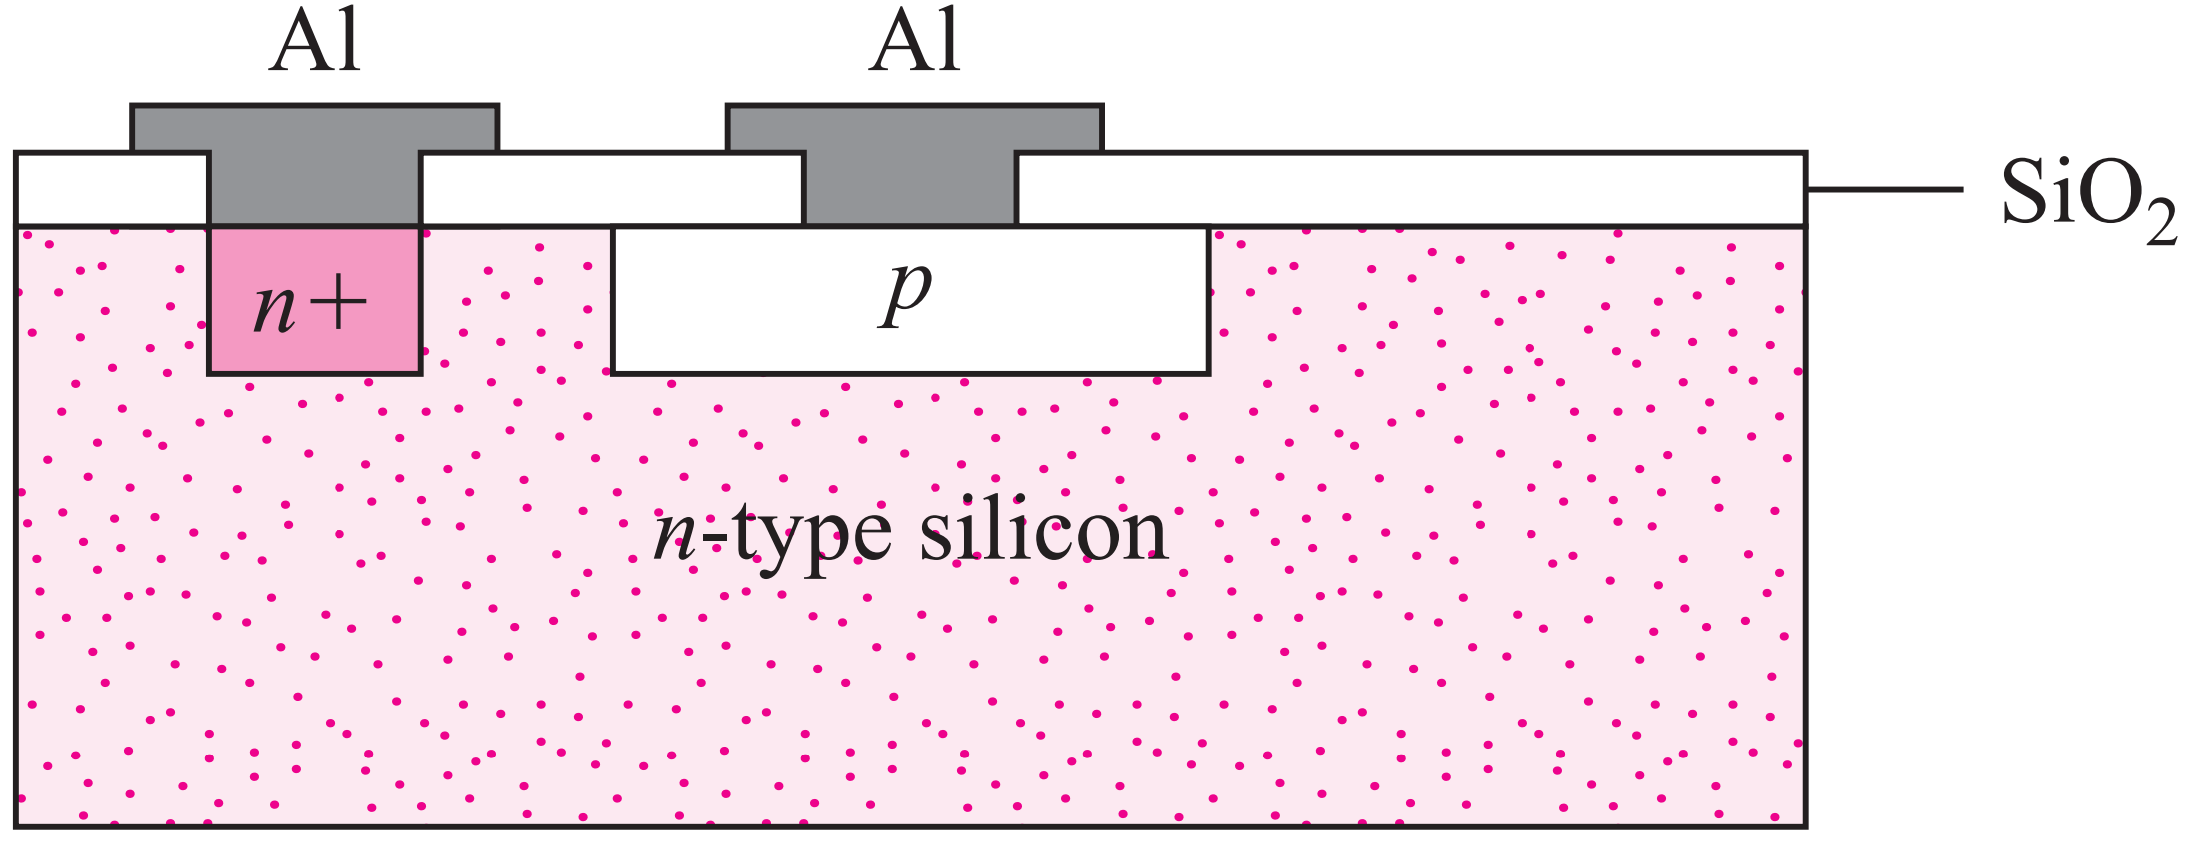
\includegraphics[width=0.45\linewidth]{img/transistor_costruzione.png}
    \caption{ Transistor vista frontale}    
\end{figure}

\chapter{Il Diodo}
\section{Come è fatto}

Il diodo è costruito	da	una	giunzione	di	silicio	di	tipo	p	e	n.
\begin{figure}[htbp]
    \centering
    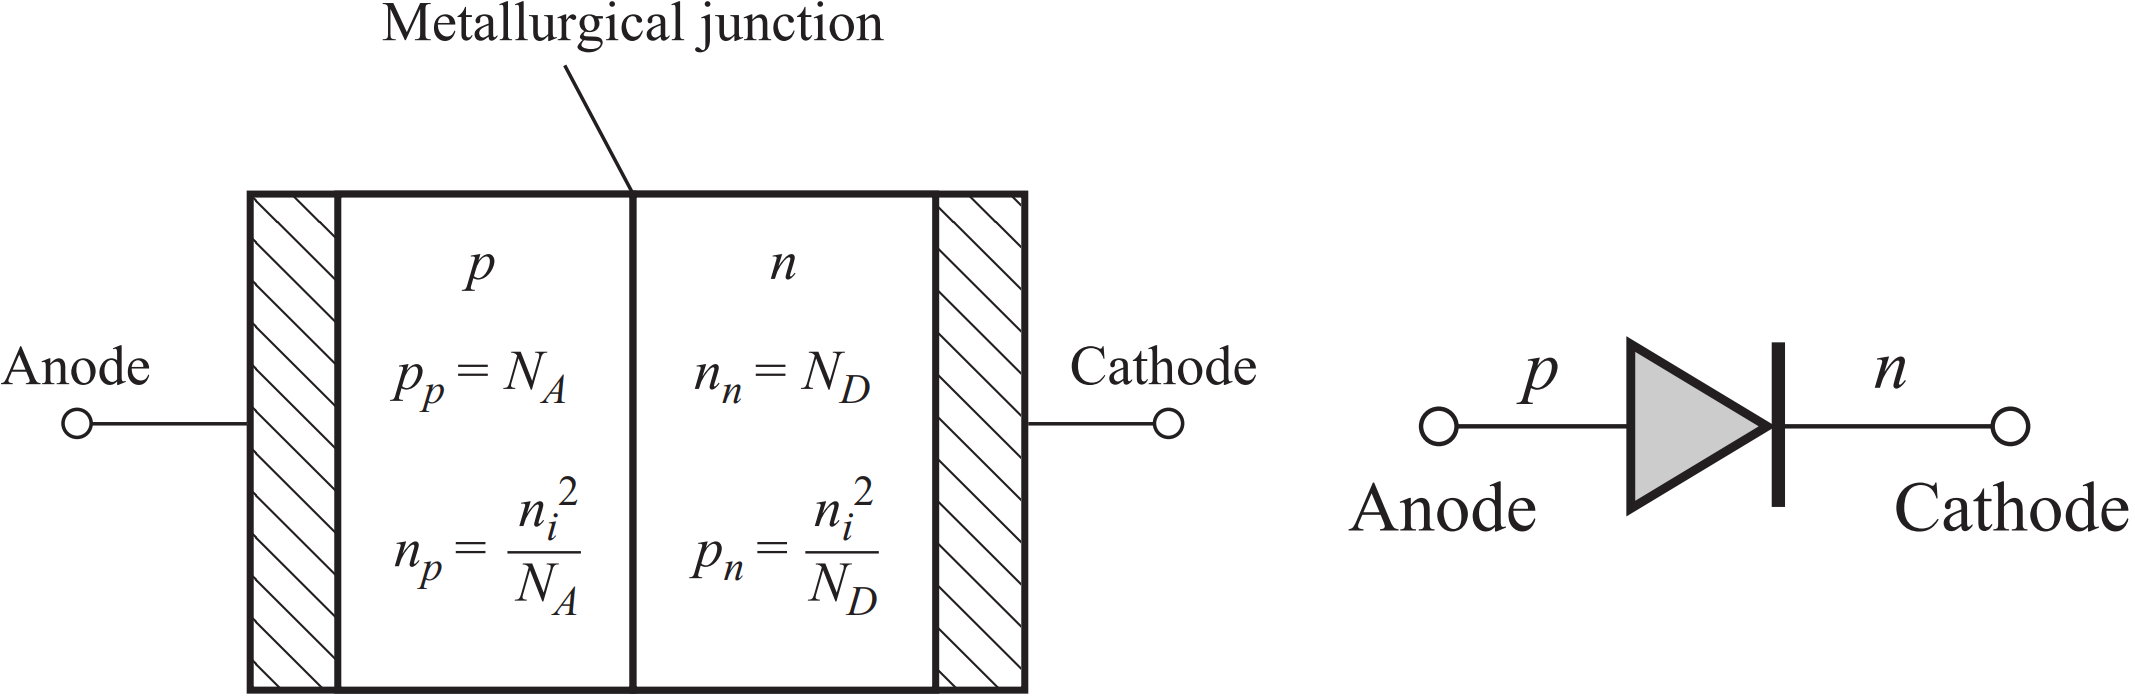
\includegraphics[width=0.65\linewidth]{img/diodo.png}
    \caption{Diodo}    
\end{figure}

Supponiamo 
\begin{itemize}
    \item $N_a = p_p= 10^{17}/cm^3\qquad N_D = n_n= 10^{16}/cm^3$
    \item $n_p = 10^{3}/cm^3\qquad p_n = 10^{4}/cm^3$
\end{itemize}

C’è	un	forte	gradiente	di	concentrazione	di	carica, infatti le	lacune	tendono	a	diffondere	dalla	zona	p alla zona n, mentre  gli	elettroni	tendono	a	diffondere	dalla	zona	n alla zona p.

\subsubsection{Carica	spaziale: } La	corrente	totale	deve	però	essere	nulla, infatti una corrente	di	drift deve	bilanciare	quella	di	diffusione. La corrente di drift è dovuta alla	creazione	di	una	regione	di	carica	spaziale,	
che	genera	un	campo	elettrico.



\begin{figure}[htbp]
    \centering
    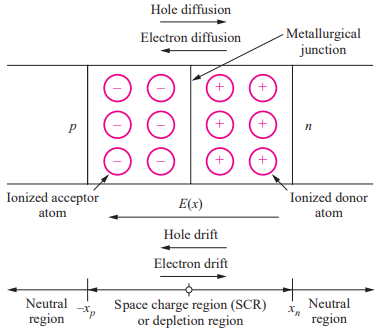
\includegraphics[width=0.45\linewidth]{img/corrente_spaziale.png}  
    
\end{figure}
\paragraph{}
Da dove viene il campo elettrico? A sinistra vi erano le lacune che si sono spostate nella parte n ed hanno lasciato degli atomi di Boro scoperti, questo fa si che si lasciano degli atomi ionizzati negativamente a sinistra. Gli elettroni che da destra sono andati a sinistra sono ioni positivi di fosforo.

Man mano che le cariche si diffondono, a ridosso della giunzione si forma una zona di ioni che sono cariche fisse e prendono in nome di \textbf{carica spaziale}, queste cariche fisse formano un dipolo con il positivo a destra e il negativo a sinistra formando così un campo elettrico dovuto a queste cariche.

Il CE fa insorgere una corrente di trascinamento che va in verso opposto a quelle della diffusione (il CE va dalle cariche positive a quelle negative, la corrente di diffusione il contrario).

\paragraph{}
Dunque all'inizio si forma la corrente di diffusione, e inizia a formarsi la carica spaziale a ridosso della giunzione e quest'ultima ostacola la diffusione ed ad un certo punto si arriva ad un equilibrio.

Questo equilibrio non significa che non c'è più movimento ma le cariche che diffondono e driftano si annullano a vicenda e dunque la corrente totale diventa nulla.

\begin{figure}[htbp]
    \centering
    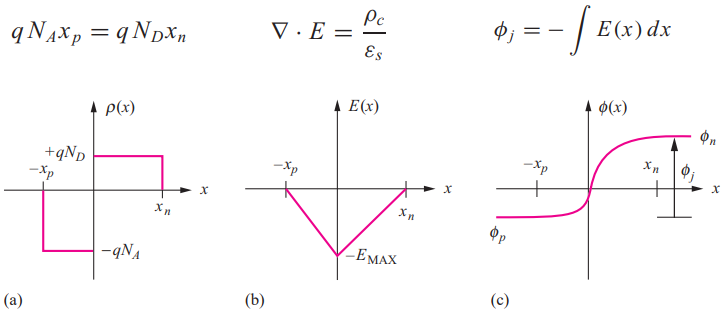
\includegraphics[width=0.9\linewidth]{img/carica_sapzoale_2.png}   
    
\end{figure}

Per capire quando questo processo va in equilibrio possiamo calcolare il campo elettrico. Possiamo calcolarlo perché la quantità di questi ioni, concentrazione, la sappiamo a priori dato che li abbiamo inseriti noi consapevolmente, sotto l'ipotesi che si siano tutti ionizzati.

\section{Calcolo del potenziale di built-in $\phi_j$}
Il potenziale di \textbf{built-in} è il fenomeno che si oppone alla diffusione delle cariche tra una zona e l'altra, viene chiamato di built-in perché è già all'interno dopo la giunzione dei due materiali con drogaggi diversi.
\paragraph{}
Sarà necessario \textbf{superare} questo potenziale per far scorrere una corrente all'interno del diodo facendolo lavorare come un corto circuito.

\paragraph{}
Utilizzando l'equazione \ref{eq_eine} e ponendola uguale a zero, dato che la corrente si deve bilanciare, avremo che:

\begin{equation*}
    E - V_T\frac{1}{p}\frac{\partial p}{\partial x} = 0 \qquad\longrightarrow\qquad E = -\frac{\partial V}{\partial x}
\end{equation*}
\begin{equation*}
    -\frac{\partial V}{\partial x} = V_T\frac{1}{p}\frac{\partial p}{\partial x}\qquad\longrightarrow\qquad dV = -V_T\frac{dp}{p}
\end{equation*}

integrando da ambo le parti otteniamo che:

\begin{equation}
    V_2 - V_1 = \phi_j = V_T\cdot \ln\biggl(\frac{N_AN_D}{n_i^2}\biggl)
\end{equation}

\newpage
dove:
\begin{itemize}
    \item $N_A \text{ e } N_D$ li conosciamo dato che abbiamo deciso noi le impurità
    \item $n_i$ dipende dalla temperatura
    \item $V_T$ è una costante
\end{itemize}
\begin{equation*}
    \phi_j = 0.026\ln(10^{17}10^{16}/10^{20}) = 0.026\ln(10^{13}) \approx 0.7V
\end{equation*}

Questo potenziale di built-in $\phi_j$ risulta essere circa $0.75V$ per il silicio e $0.3V$ per il germanio, tensione che contrasta la diffusione delle cariche dei portatori.

Questo significa che una lacuna a sinistra deve avere abbastanza energia per superare la barriera di potenziale.

\section{Potenziale esterno}

Applicando	un	potenziale	esterno	si	altera	l'equilibrio.

\begin{itemize}
    \item Un	\textbf{potenziale	positivo}	riduce	la	barriera,	e	una	corrente	può	scorrere	nel	diodo
    \item Un	\textbf{potenziale	negativo}	incrementa	la	barriera.	La	corrente	scorre,	ma	è	molto	piccola	perché	fatta	solo	dai	portatori	minoritari
\end{itemize}

Per la legge della sovrapposizione degli effetti il potenziale esterno si somma a quello interno.

\begin{figure}[htbp]
    \centering
    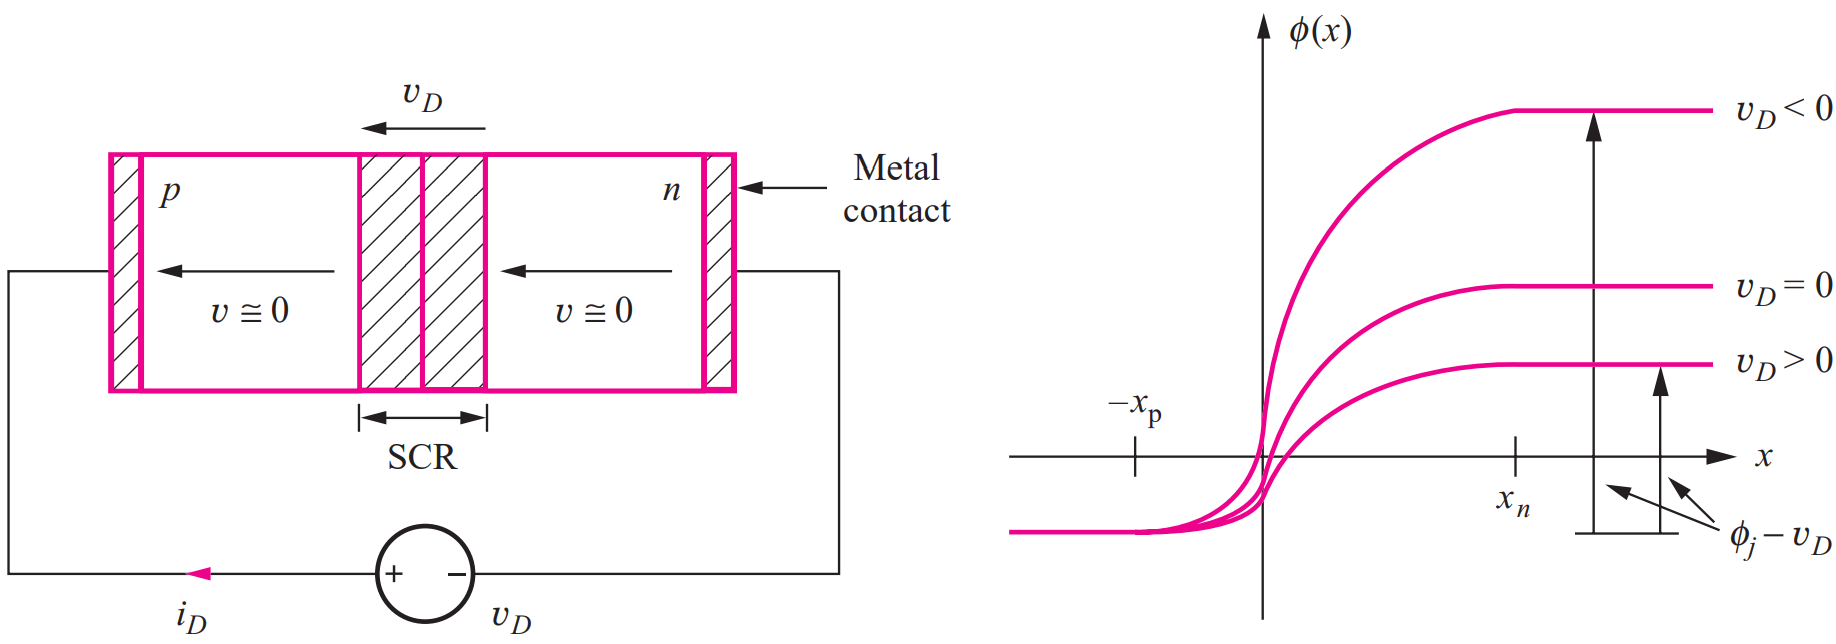
\includegraphics[width=0.9\linewidth]{img/pote_est.png}
    
    
\end{figure}

La barriera si può molto facilmente abbassare o azzerare, basta applicare una differenza di potenziale tra anodo e catodo di $0.7V$ e a questo punto tutte le cariche possono spostarsi liberamente.

\subsection{Potenziale	positivo}
L'equilibrio	è	perturbato,	la	regione	di	carica	spaziale	si	restringe, inoltre passerà molta corrente in quanto la differenza di densità di carica è di diversi ordini di grandezza superiore.

La	corrente	di	drift non	è	in	grado	di	bilanciare	quella	di	diffusione dunque:
\begin{itemize}
    \item le lacune si	diffondono	dalla	zona	p	alla	zona	n;
    \item gli elettroni si	diffondono	dalla	zona	n	alla	zona	p;
    \item le correnti fluiscono nello stesso verso.
\end{itemize}

\newpage
\subsection{Potenziale	negativo}
In questo caso mettiamo una batteria in polarità inversa: il $+$ sul catodo e il $-$ sull'anodo. Così facendo non solo le cariche sono contrastate dalla barriera di spostamento ma vi è anche la barriere aggiuntiva della batteria collegata e dunque le cariche non diffondono per niente e non passa corrente.

\paragraph{}
La	barriera	di	potenziale	si	amplia, la	regione	di	carica	spaziale	si	allarga. La	corrente	di	diffusione	viene	ostacolata,	mentre	i	portatori	minoritari	possono	scivolare	per	la	barriera:

\begin{itemize}
    \item le lacune si	diffondono	dalla	zona	n	alla	zona	p;
    \item gli elettroni si	diffondono	dalla	zona	p	alla	zona	n.
\end{itemize}

Scorre	quindi	una	debole	corrente,	dovuta	ai	portatori minoritari	generati	termicamente, in	prima	approssimazione	indipendente	dal	potenziale, talmente piccola che può essere considerata nulla.

\paragraph{}
Il diodo a differenza di un resistore permette di dare un solo verso alla corrente, \textbf{raddrizzarla}: infatti si para di \textbf{polarizzazione}.

\begin{itemize}
    \item \textbf{Polarizzazione diretta}: tensione esterna applicata in modo da ridurre la barriera energetica permettendo il flusso di corrente;
    \item \textbf{Polarizzazione inversa}: tensione esterna applicata in modo da aumentare la barriera energetica impedendo il flusso di corrente.
\end{itemize}


\begin{figure}[htbp]
    \centering
    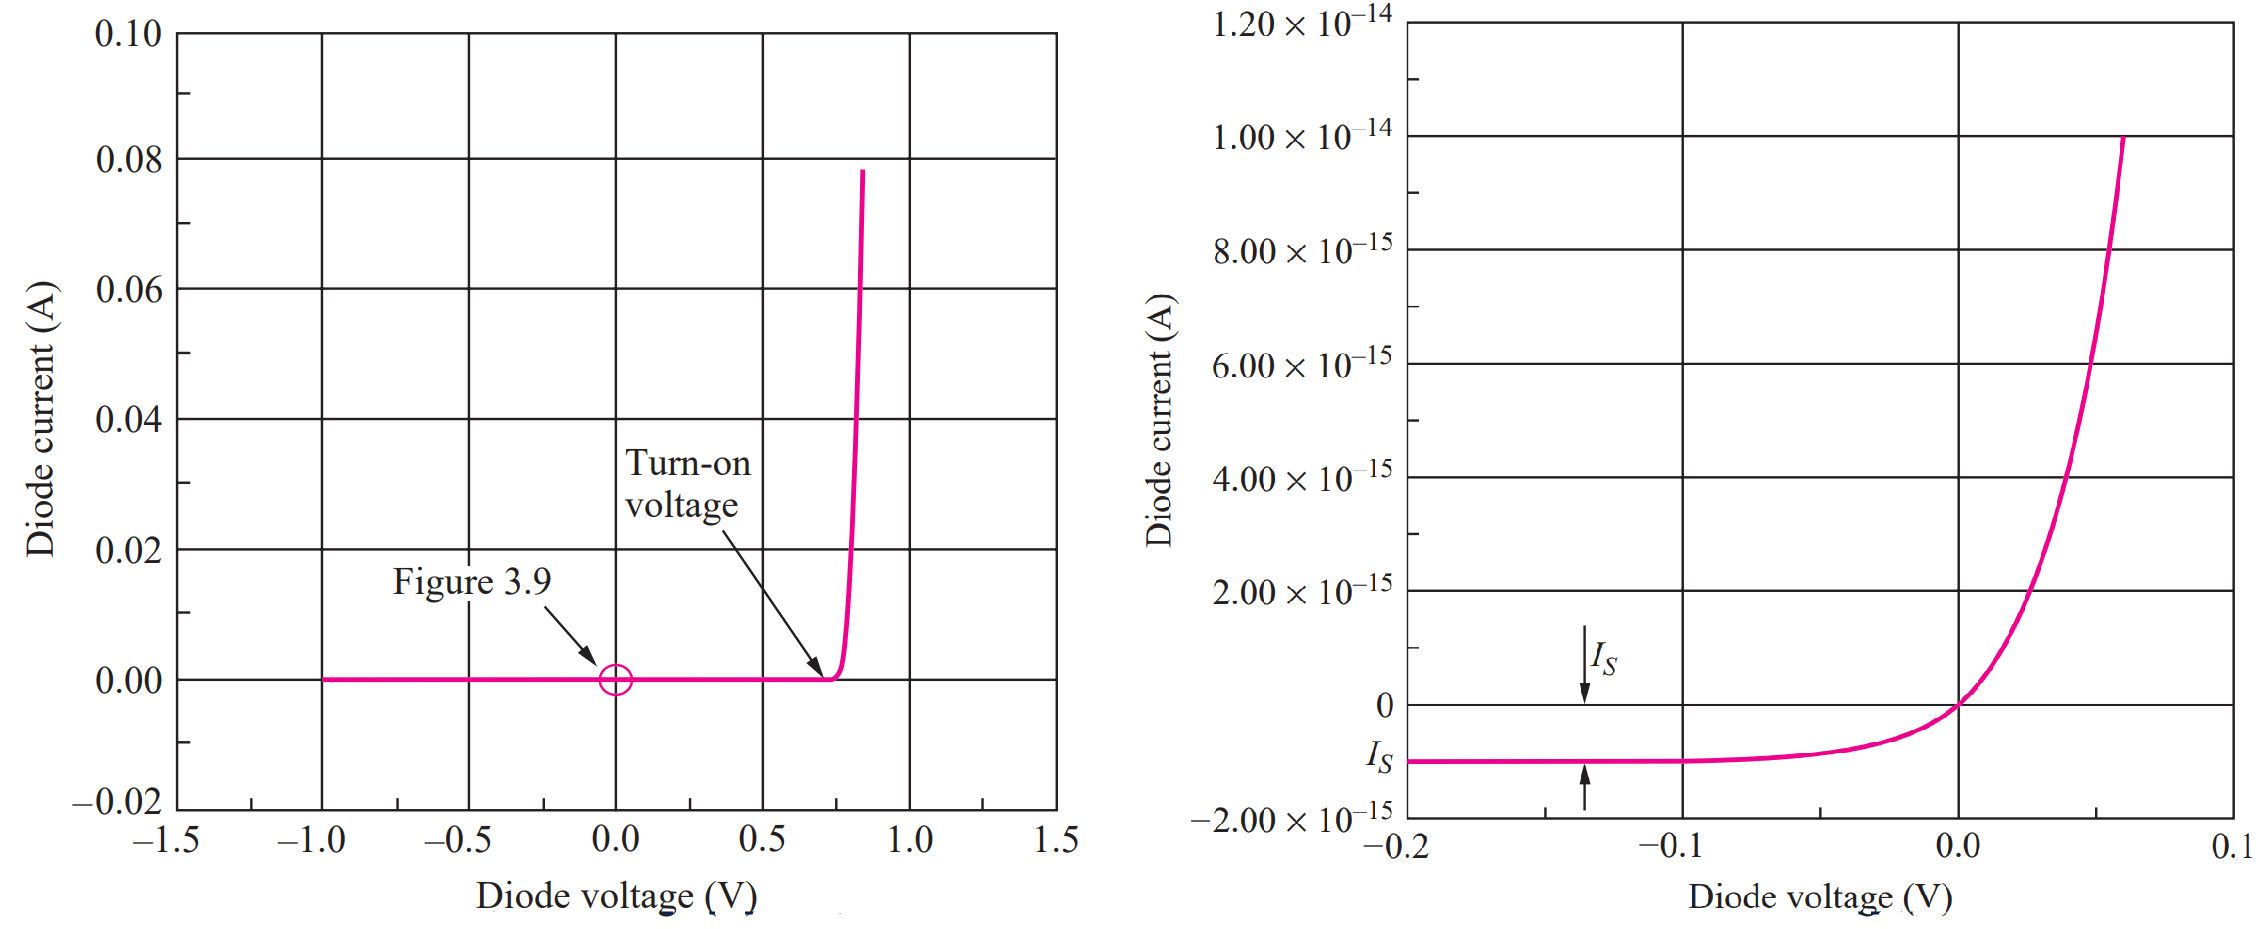
\includegraphics[width=0.97\linewidth]{img/potenziale_diodoi.png}
    \caption{Grafico andamento tensione-corrente}
    
\end{figure}

\newpage
\section{Modello matematico del Diodo}

\begin{equation}
    I_D = I_S\biggl[\exp{\biggl(\frac{qv_D}{nkT}\biggl)-1}\biggl] = I_S\biggl[\exp{\biggl(\frac{v_D}{nV_T}\biggl)-1}\biggl]
\end{equation}

Dove

\begin{itemize}
    \item $I_S$ =	corrente	inversa	di	saturazione
    \item $v_D$ =	tensione	applicata	ai	capi	del	diodo
    \item q = carica elettrone $1.6\cdot10^{-19} \text{ [C]}$
    \item k = costante	di	Boltzmann $1.38\cdot10^{-23} \text{ [J/K]}$
    \item n	=	fattore	di	non	idealità	(tipicamente	1 per Si)
    \item $V_T = kT/q$ = tensione termica (0.025V, Si, temp. amb)
\end{itemize}


\section{Modello di diodo ideale per grandi tensioni}
Quando si lavora con tensioni molto maggiori della tensione minima per far oltrepassare la barriera alle cariche (0.7V) allora possiamo applicare una prima approssimazione generale del diodo:
\begin{figure}[htbp]
    \centering
    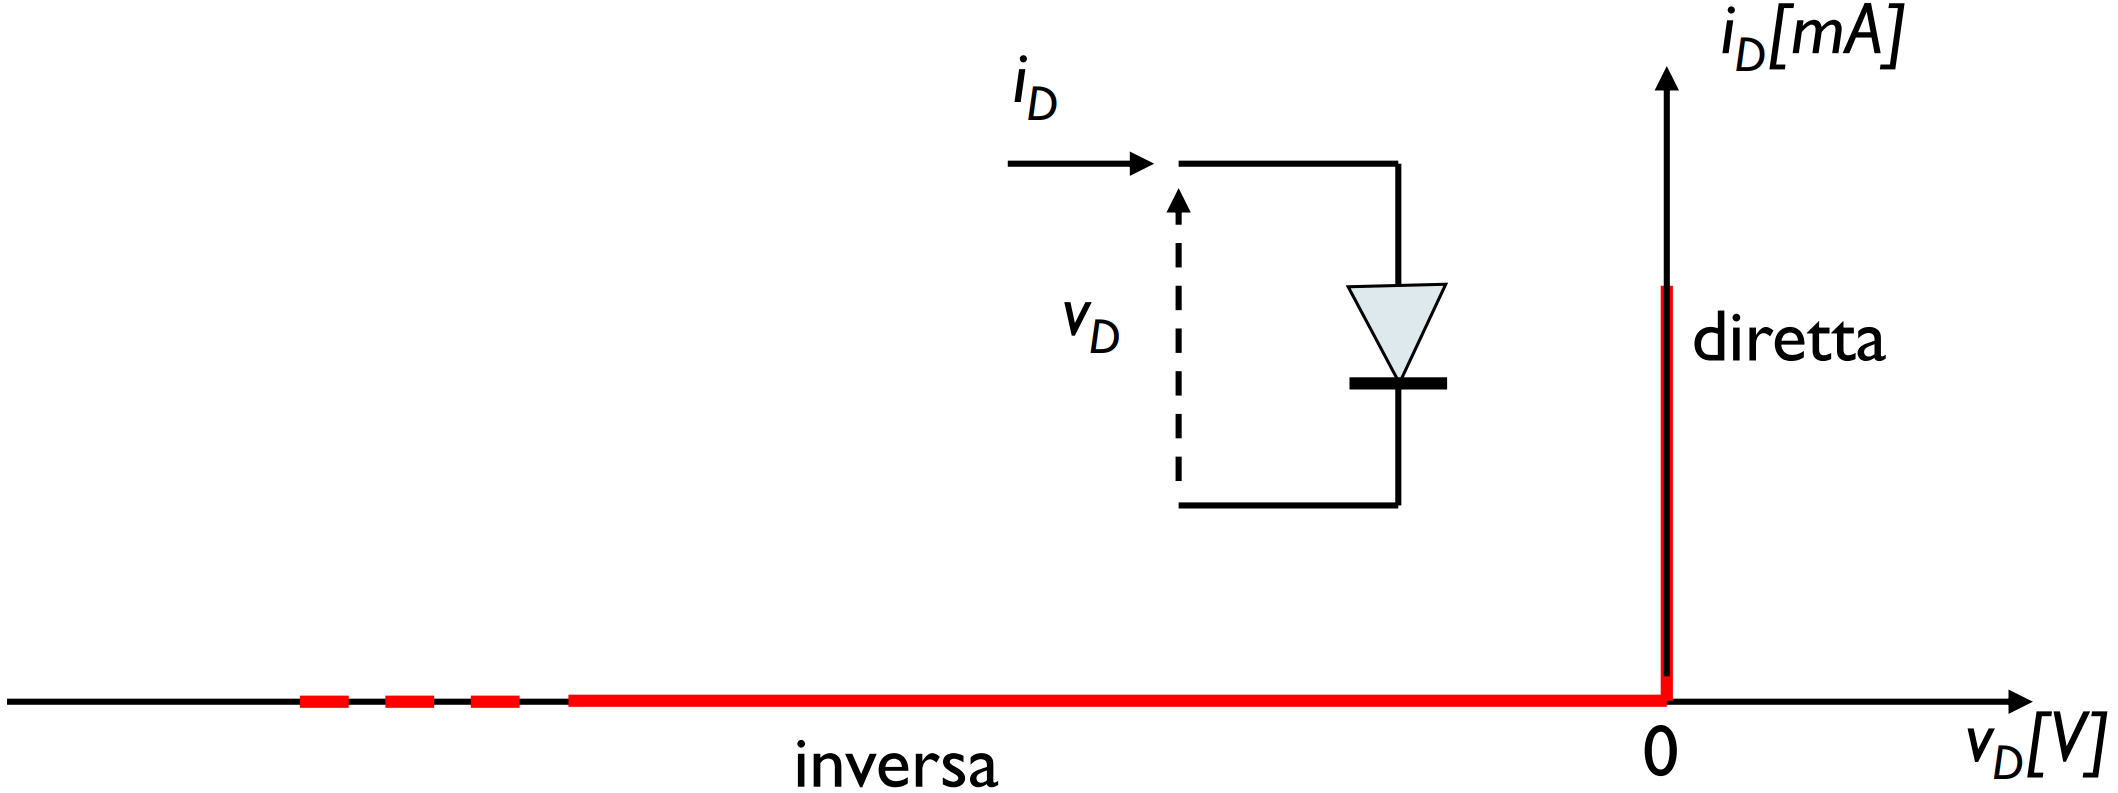
\includegraphics[width=0.65\linewidth]{img/diodo_Ideale.png}
    \caption{Diodo ideale}    
\end{figure}

\paragraph{}
Questa grossolana approssimazione è applicabile se il nostro circuito è sottoposto a decine di volt.
\begin{figure}[htbp]
    \centering
    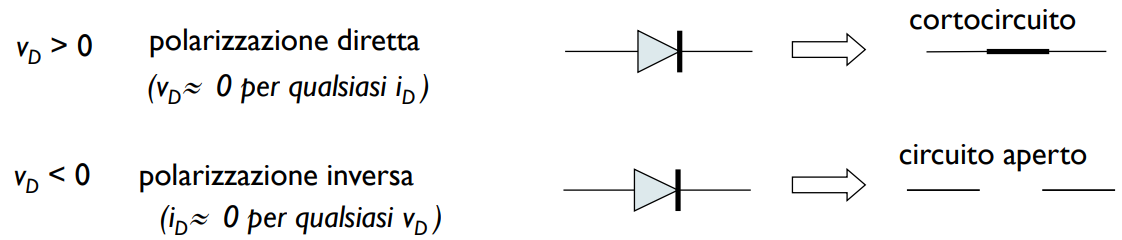
\includegraphics[width=0.77\linewidth]{img/approx_diodo.png}
    \caption{Comportamento in una rete}    
\end{figure}


\section{Diodo nei circuiti}

I diodi sono dei componenti molto utilizzati soprattutto negli alimentatori di apparecchiature elettroniche in quanto esse, funzionando in regime di corrente continua, hanno bisogno di rendere positiva la sinusoide di rete per poter poi estrarre, grazie ad un condensatore, la componente continua.
\paragraph{}
Vediamo alcuni esempi di circuiti.
\newpage
\subsection{Rettificatore a semi onda}
Il diodo è molto utilizzato per raddrizzare la sinusoide di rete.

\begin{figure}[htbp]
    \centering
    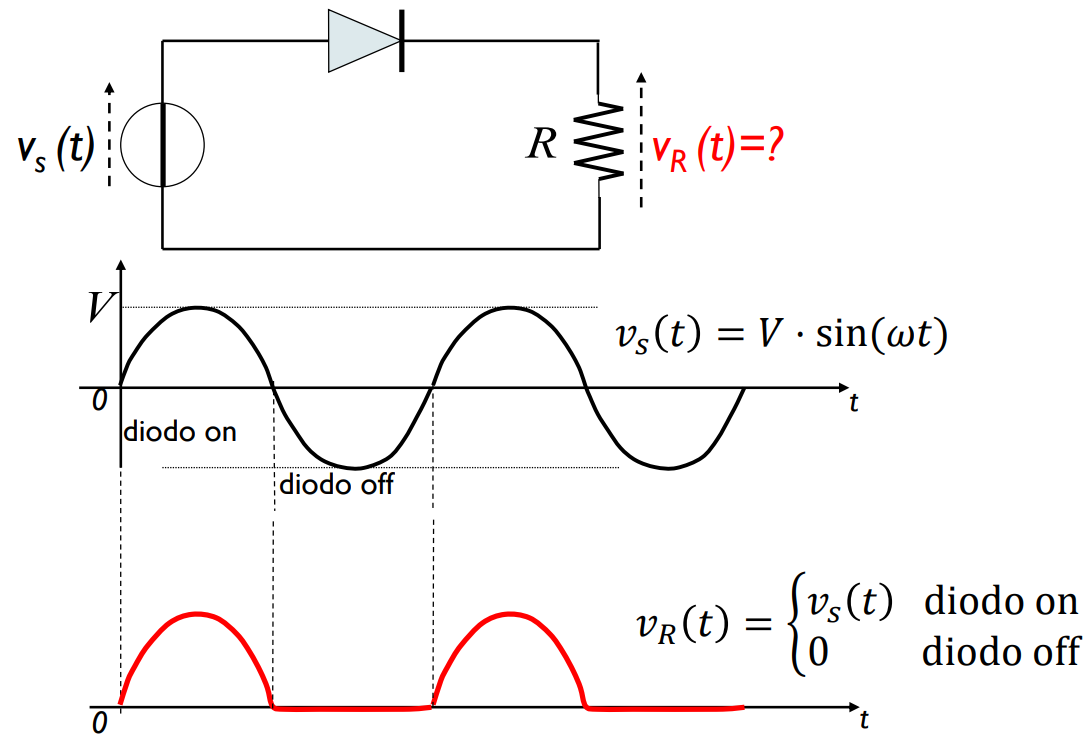
\includegraphics[width=0.7\linewidth]{img/rettificatore.png}
    \caption{Rettificatore a semi onda}    
\end{figure}

\paragraph{}
\subsection{Rettificatore ad onda intera, il ponte di diodi}
Ovviamente possiamo raddrizzare tutta la sinusoide di rete in una sinusoide con soli semi onde positive, grazie al ponte di diodi:

\begin{figure}[htbp]
    \centering
    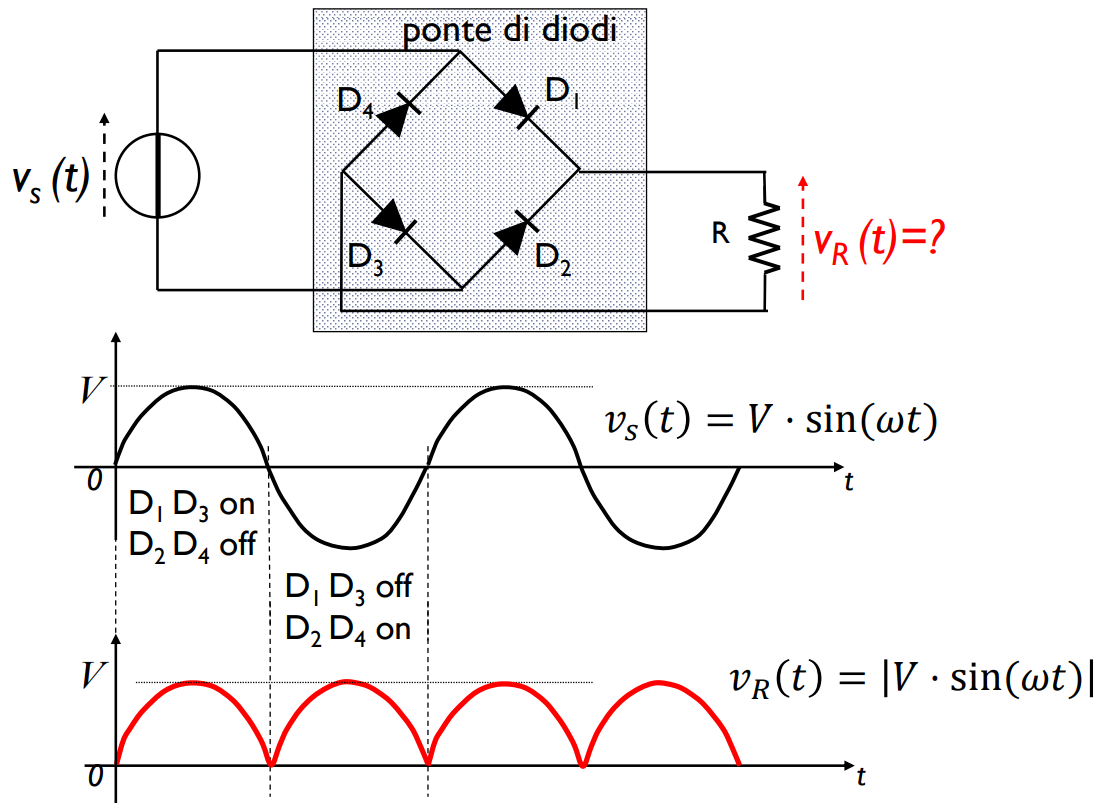
\includegraphics[width=0.65\linewidth]{img/ponte_diodi.png}
    \caption{Ponte di diodi}
    
\end{figure}

\paragraph{}
\subsection{Raddrizzatore AC/DC con filtro capacitivo}
Normalmente i dispositivi elettronici funzionano in corrente continua. La rete però fornisce una tensione sinusoidale a 50Hz.
Grazie al seguente circuito possiamo far tendere la nostra sinusoide di rete ad una tensione costante.

\begin{figure}[htbp]
    \centering
    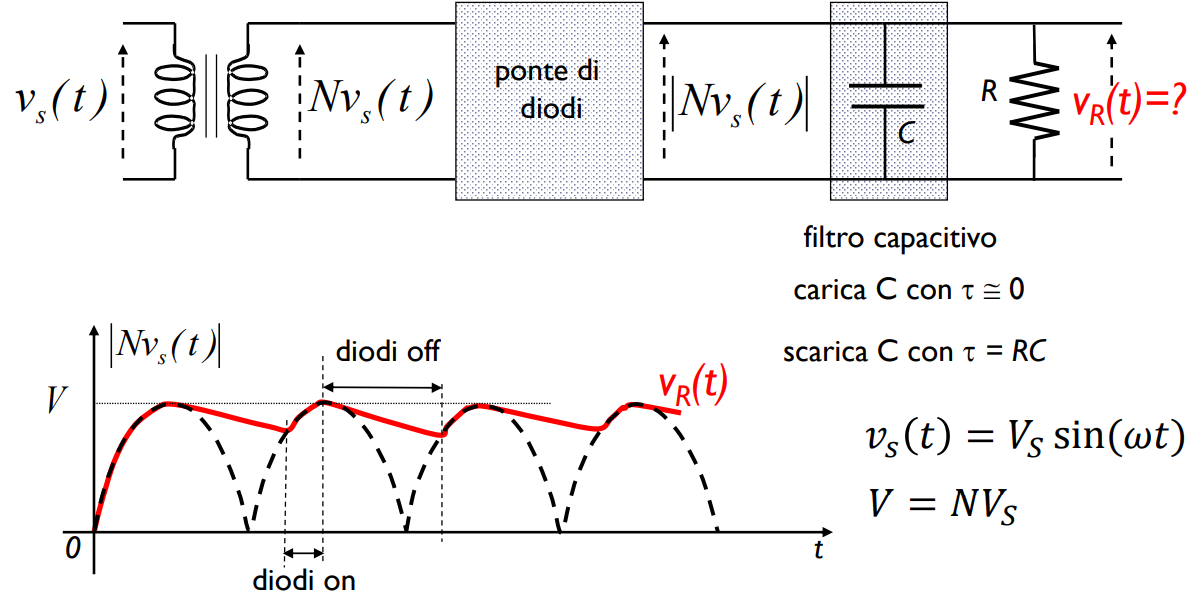
\includegraphics[width=0.75\linewidth]{img/raddrizzatore.png}
    \caption{Raddrizzatore AC/DC con filtro capacitivo}    
\end{figure}

La fluttuazione della tensione di uscita $V_R(t)$ può essere controllata
modificando la costante di tempo di scarica $\tau = RC$ ($>>T$)
\paragraph{}
Più il condensatore è grosso più riesce a mantenere costante la tensione durante la scarica, dunque perché non utilizzarne uno con molta capacità?
\paragraph{}
Ci sono alcuni motivi per evitare l'utilizzo di un condensatore grande:

\begin{itemize}
    \item \textbf{Corrente di carica elevata:} Un condensatore di grandi dimensioni richiede una corrente di carica elevata durante l'avvio del circuito. Questo può causare picchi di corrente eccessivi che possono danneggiare i diodi raddrizzatori e altri componenti del circuito.
    \item \textbf{Tempo di carica lungo:} Un condensatore di grandi dimensioni impiega più tempo per caricarsi. Questo può portare a un ritardo significativo nella tensione di uscita all'accensione del circuito.
    \item \textbf{Aumento del ripple:} Un condensatore di grandi dimensioni può aumentare il ripple della tensione di uscita. Il ripple è la componente alternata residua presente nella tensione continua dopo la raddrizzatura. Un ripple eccessivo può essere dannoso per i circuiti elettronici sensibili.
    \item \textbf{Dimensioni e costo:} Un condensatore di grandi dimensioni è più grande e costoso di un condensatore di dimensioni più ridotte.

    \item \textbf{Non adatto a carichi variabili:} Un condensatore di grandi dimensioni non è adatto a carichi variabili. Se il carico varia, la tensione di uscita varierà di conseguenza.
\end{itemize}

In generale, è consigliabile utilizzare un condensatore di dimensioni sufficienti per ridurre il ripple a un livello accettabile, ma non troppo grande da causare i problemi sopra menzionati. Il valore ottimale del condensatore dipende da diversi fattori, tra cui la frequenza della tensione di rete, il tipo di raddrizzatore, il valore del carico e il livello di ripple desiderato.


\newpage
\section{Modello di diodo ideale per piccole tensioni}

A differenza di prima ora stiamo prendendo in esame un circuito che lavora su basse tensioni (es. 5V). Per questo utilizzo non si può approssimare come prima in quanto la barriera di potenziale iniziale diventa molto rilevante e potrebbe creare problemi ai carichi che si attaccano al circuito.

\begin{figure}[htbp]
    \centering
    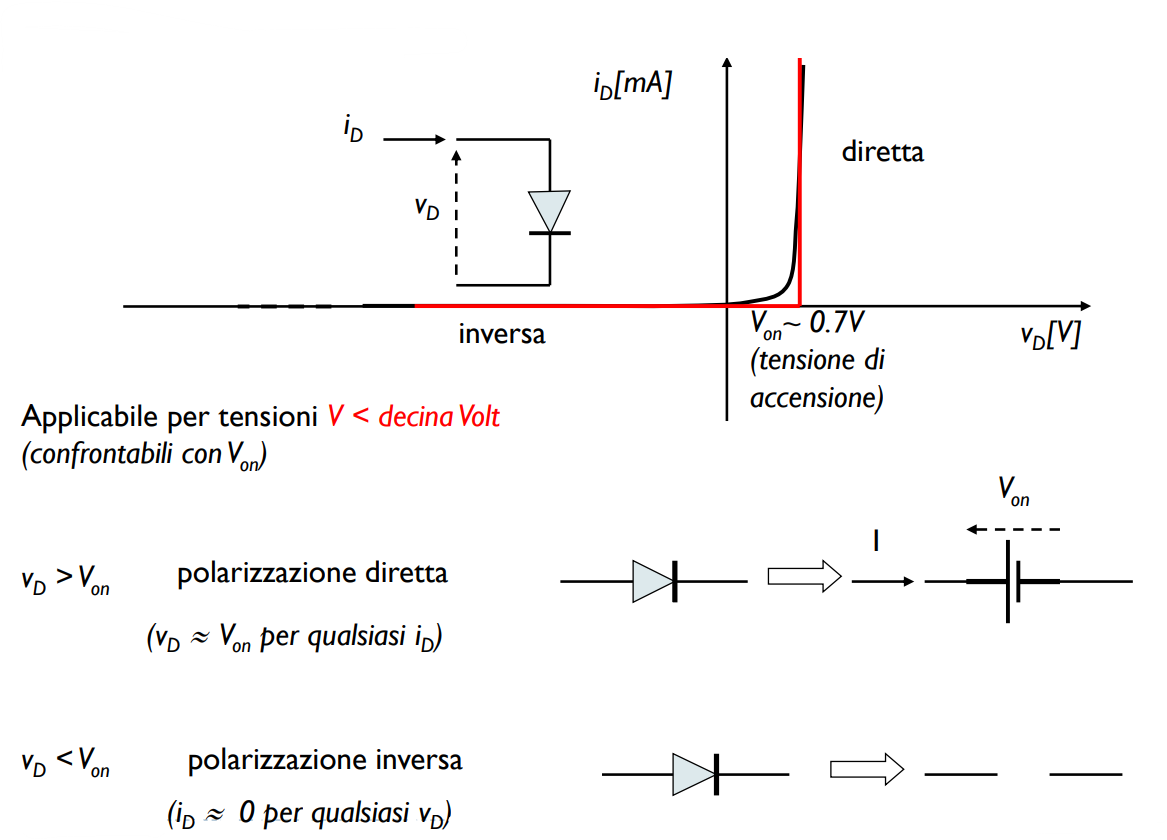
\includegraphics[width=0.8\linewidth]{img/piccole_tens.png}
    \caption{Modello di diodo per piccole tensioni}    
\end{figure}

\section{I circuiti logici realizzabili con i diodi}
I diodi possono essere utilizzati per costruire porte logiche quali ad esempio la AND e OR.
\paragraph{}

Di seguito verrà mostrata una loro possibile implementazione.
\newpage
\subsection{Circuito AND}

\begin{figure}[htbp]
    \centering
    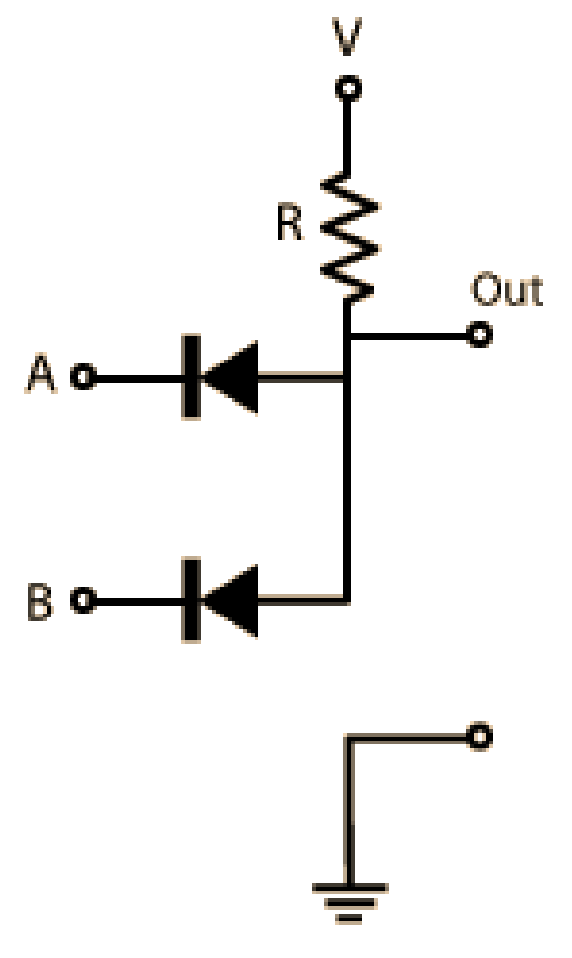
\includegraphics[width=0.17\linewidth]{img/and.png}
    \caption{Diode AND gate}
    
\end{figure}

Vediamo i tre casi:

\begin{itemize}
    \item $V_A = V_B = 5V$
    \begin{itemize}
        \item entrambi i diodi sono interdetti
        \item non scorre corrente 
        \item l'uscita va a 5V
    \end{itemize}
    \item $V_A = 0V,  V_B = 5V$
    \begin{itemize}
        \item Il diodo B conduce, il diodo A è interdetto
        \item l'uscita scende a $V_{on}$ (0 per grandi tensioni)
    \end{itemize}
    \item $V_A = V_B = 0V$
    \begin{itemize}
        \item entrambi i diodi conducono
        \item l'uscita scende a $V_{on}$ (0 per grandi tensioni)
    \end{itemize}
\end{itemize}

\subsection{Circuito OR}
\begin{figure}[htbp]
    \centering
    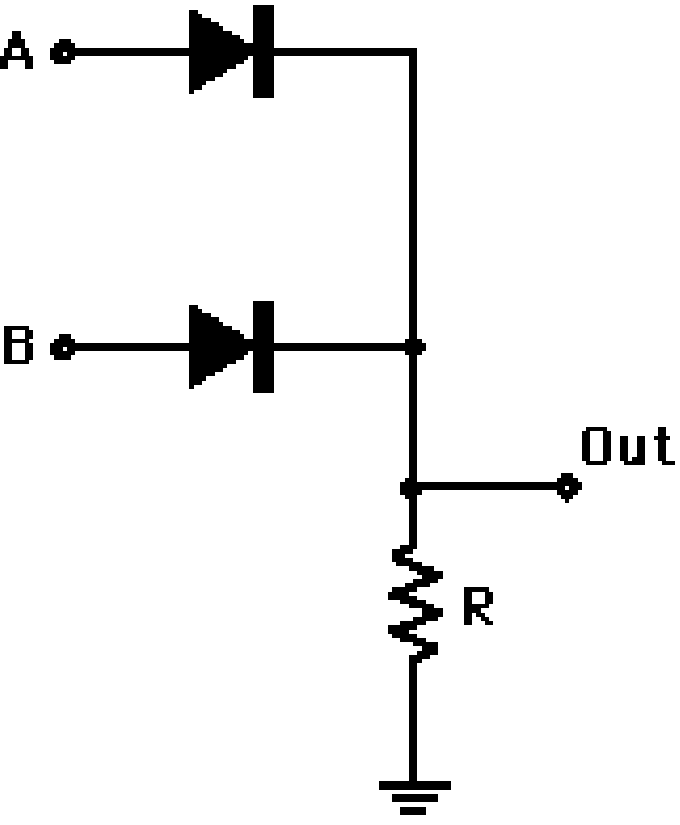
\includegraphics[width=0.17\linewidth]{img/OR_GATE.png}
    \caption{Diode OR gate}
    
\end{figure}

Vediamo i tre casi:

\begin{itemize}
    \item $V_A = V_B = 5V$
    \begin{itemize}
        \item entrambi i diodi conducono
        \item l'uscita va a 5V - $V_{on}$ (5 per grandi tensioni)
    \end{itemize}
    \item $V_A = 5V,  V_B = 0V$
    \begin{itemize}
        \item Il diodo A conduce, il diodo B è interdetto
        \item l'uscita va a 5V - $V_{on}$ (5 per grandi tensioni)
    \end{itemize}
    \item $V_A = V_B = 0V$
    \begin{itemize}
        \item entrambi i diodi sono interdetti
        \item l'uscita scende a 0V (0 per grandi tensioni)
    \end{itemize}
\end{itemize}



 \chapter{Dispositivi MOSFET}
\section{Cos'è il condensatore MOS}
Partiamo dal nome:
\begin{itemize}
    \item MOS: Metal–Oxide–Semiconductor
    \item FET: field–effect transistor
\end{itemize}
ovvero transistore metallo-ossido-semiconduttore ad effetto di campo, questo dispositivo è alla	base	dei	circuiti	a	MOSFET.

\section{Come è fatto}
Costituito	da	un	layer conduttore	detto	\textbf{gate},	separato	da	un	
substrato in	silicio	drogato	(di	tipo	p	o	n) e	da	uno	strato	isolante
di	biossido	di	silicio ($SiO_2$), utilizzato	per	indurre	una	carica	superficiale	all'interfaccia	tra	il	
silicio	e	il	biossido	di	silicio.

\begin{figure}[htbp]
    \centering
    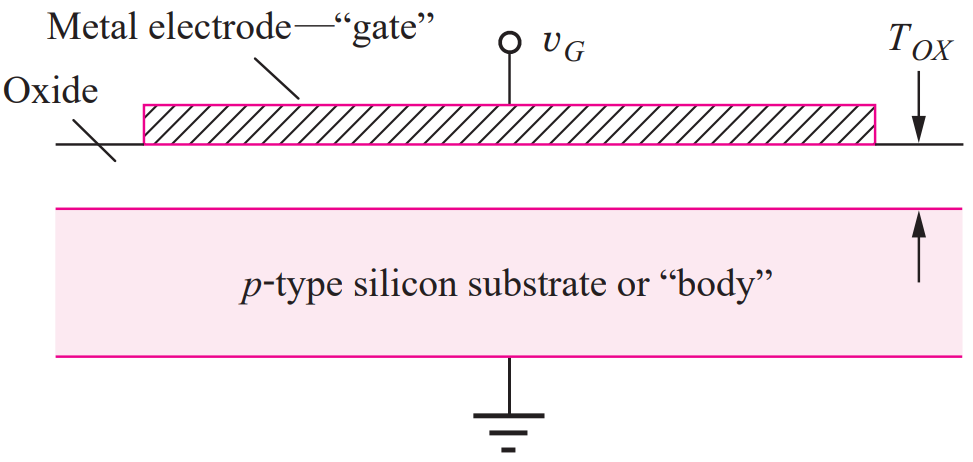
\includegraphics[width=0.4\linewidth]{img/cond_mos.png}
    \caption{Condensatore MOSFET}    
\end{figure}

Ricorda proprio un condensatore a piatti, tranne che al posto di esserci un metallo da entrambe le facce troviamo un semiconduttore e un metallo, dunque alteriamo le normali caratteristiche di un condensatore.

\subsection{Regione	di	accumulazione}
La polarizzazione negativa avviene quando sul gate troviamo cariche negative, mentre sotto al gate troviamo cariche positive composta da lacune.

Dunque si dice che la superficie	del	semiconduttore	è	in	accumulo. Sostanzialmente abbiamo accumulato le cariche presenti nel substrato drogato di silicio sulla sua superficie.

\begin{figure}[htbp]
    \centering
    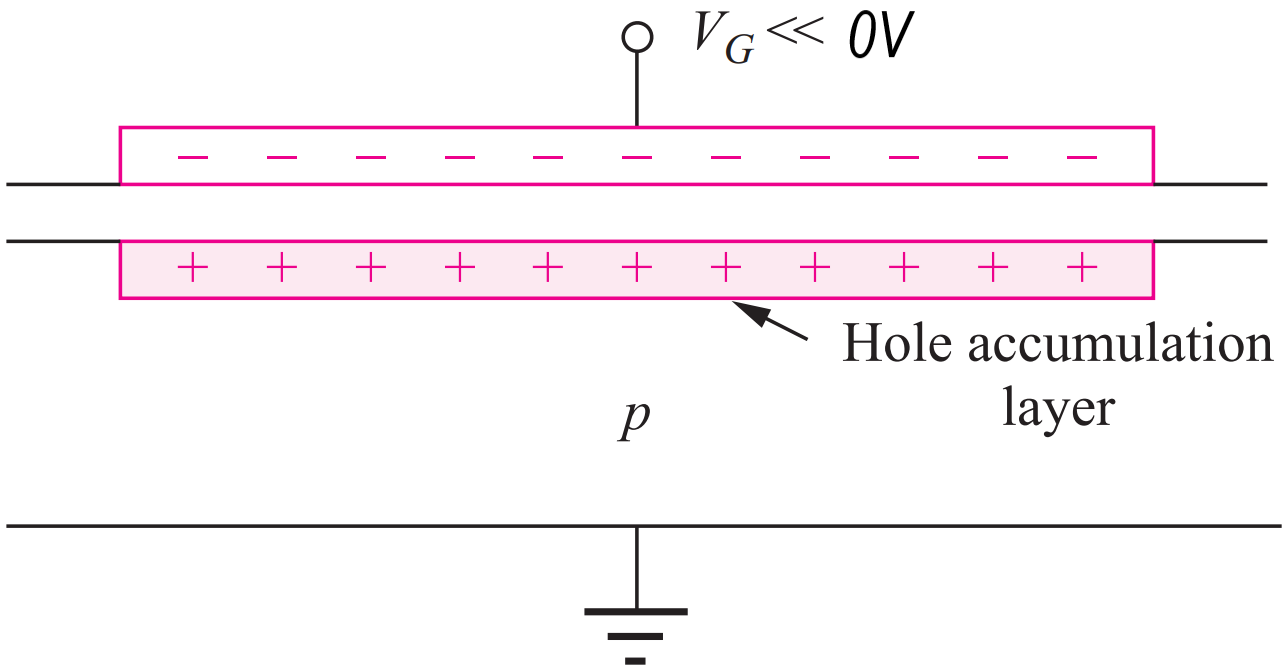
\includegraphics[width=0.4\linewidth]{img/polarizza_neg.png}  
    \caption{Regione	di	accumulazione}   
\end{figure}

\newpage
\subsection{Regione	di	svuotamento}
Il	potenziale	del	gate	viene	incrementato	(>	0V). Dunque il campo elettrico è diretto verso il basso e allontana le lacune dalla superficie. Allontana le lacune ma rimangono gli ioni negativi degli atomi accettori che abbiamo utilizzato per produrre il substrato di tipo p, i quali controbilanceranno la carica positiva che si è formata sul gate.

Dunque ecco perché il nome zona di svuotamento, perché abbiamo allontanato, svuotato, la zona dalle lacune.

Da notare che gli ioni nel substrato sono \textbf{fissi} perché fanno parte del reticolo cristallino del silicio.

\begin{figure}[htbp]
    \centering
    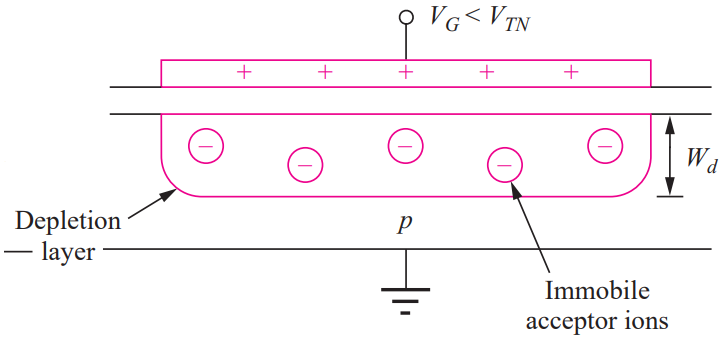
\includegraphics[width=0.47\linewidth]{img/regione_svuotmamnto.png}
    \caption{Regione	di	svuotamento}    
\end{figure}

\subsection{Regione	di	inversione}
Se aumentiamo ancora la tensione sul gate, gli elettroni sono attratti sulla superficie del substrato, dunque la carica positiva nel metallo ora viene bilanciata dagli ioni fissi e da elettroni nel substrato.
\paragraph{}
Quando il numero di elettroni supera il numero di lacune, ci troviamo in condizione della cosiddetta \textbf{inversione}. La tensione alla quale si forma lo strato	di	inversione	è	chiamata	
\textbf{tensione	di	soglia},	indicata	con	VT (o	VTN per	gli	elettroni).



\begin{figure}[htbp]
    \centering
    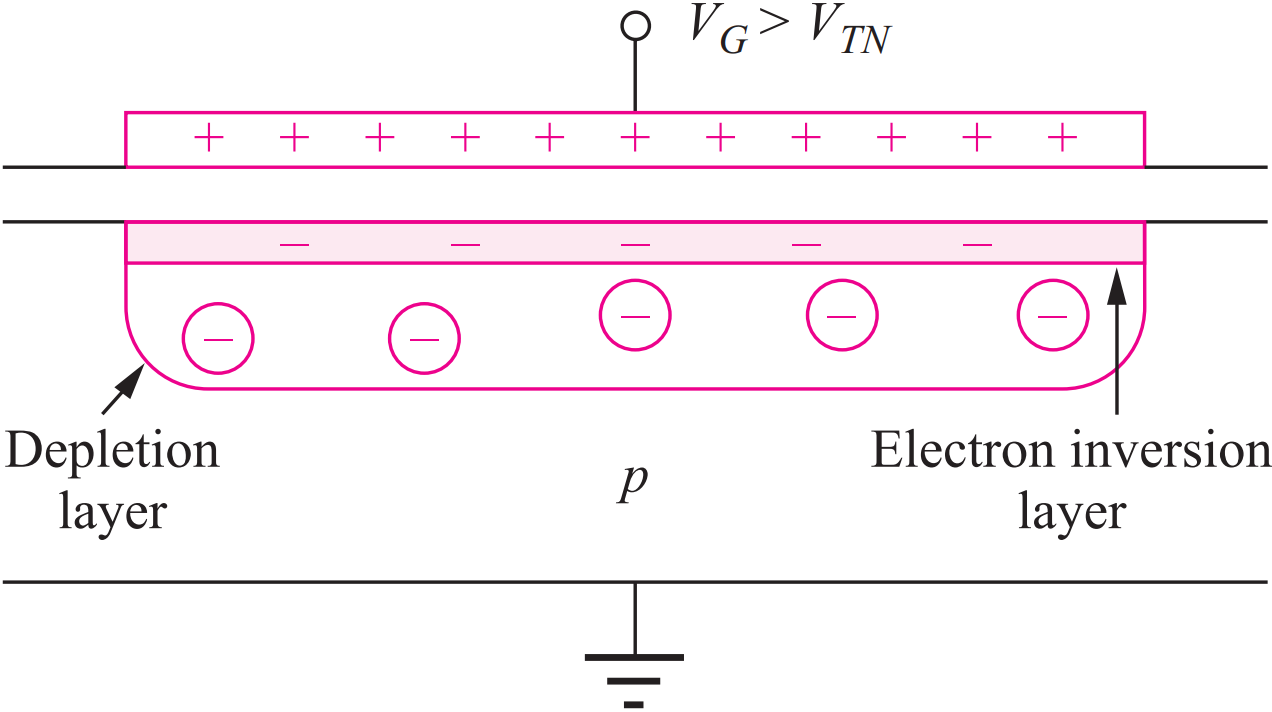
\includegraphics[width=0.4\linewidth]{img/inversione.png}
    \caption{Regione	di	inversione}
    
\end{figure}

Dunque è come se avessimo fatto uno strato di tipo n sopra le lacune del substrato, abbiamo creato uno \textbf{strato conduttore}, praticamente fatto a comando variando la tensione sul gate, che mette in contatto il lato destro e sinistro del condensatore.

Ci fa comodo questo strato, infatti ai lati possiamo mettere due terminali ed otteniamo appunto il \textbf{transistore}.

\newpage
\section{Il transistore nMOS}

Ai lati del gate, mettiamo due regioni di tipo n+ (tanti elettroni) chiamati: \textbf{source}  e \textbf{drain}.

Questi due terminali sono messi in modo tale che possano mettersi in contatto con lo strato di inversione discusso in precedenza, formando di fatto una sorta di U rovesciata.


\begin{figure}[htbp]
    \centering
    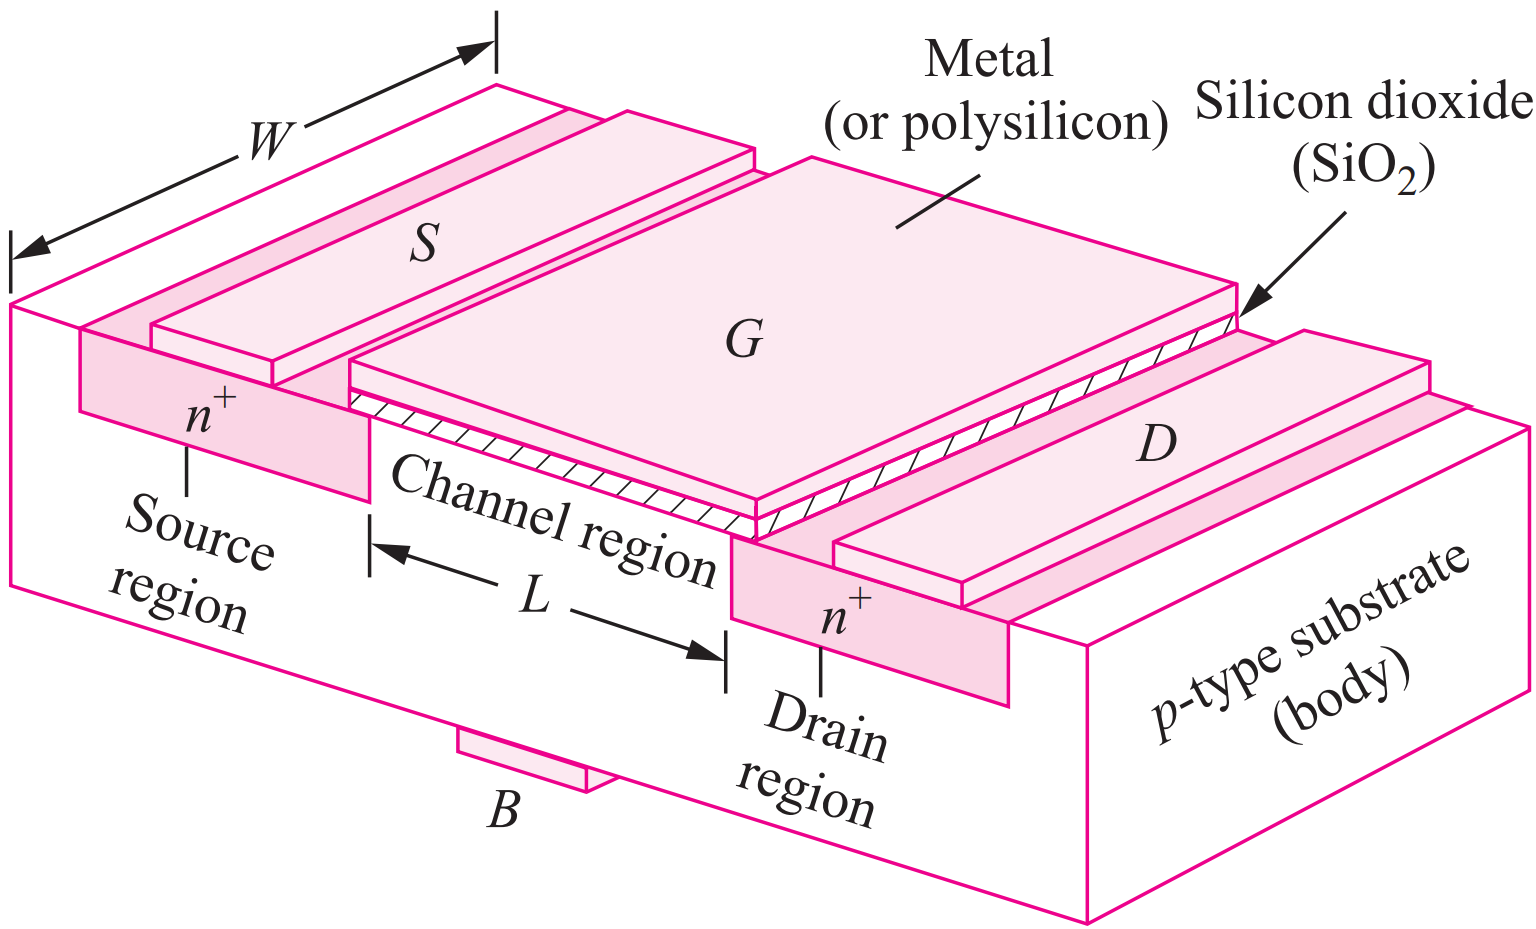
\includegraphics[width=0.5\linewidth]{img/nMOS.png}
    \caption{Transistore nMOS}    
\end{figure}

Il transistore ha due parametri molto importanti che influenzano le caratteristiche elettrice del circuito:
\begin{itemize}
    \item Distanza tra i terminali, lunghezza L del canale;
    \item Larghezza del transistore
\end{itemize}

Con più la lunghezza è piccola più il costo per stampare il circuito diventerà costoso $\approx 10nm$. Questa tipologia di transistori veniva più utilizzata una decina di anni fa, ora si è passati ad un nuovo transistore chiamato \textbf{FinFET} tridimensionale e non più planare, consentendo ulteriormente la miniaturizzazione.

\subsection{Simbolo circuitale}
Le zone di source e drain sono terminali fortemente drogate con atomi donatori, e possono anche essi donare elettroni per formare lo strato di inversione.
Le stesse regioni formano anche due diodi con il substrato (giunzione p-n), i quali sono normalmente \textbf{polarizzati inversamente}, in prima approssimazione è come se non ci fossero. Creano solo una carica spaziale introno alle due connessioni.

\begin{figure}[htbp]
    \centering
    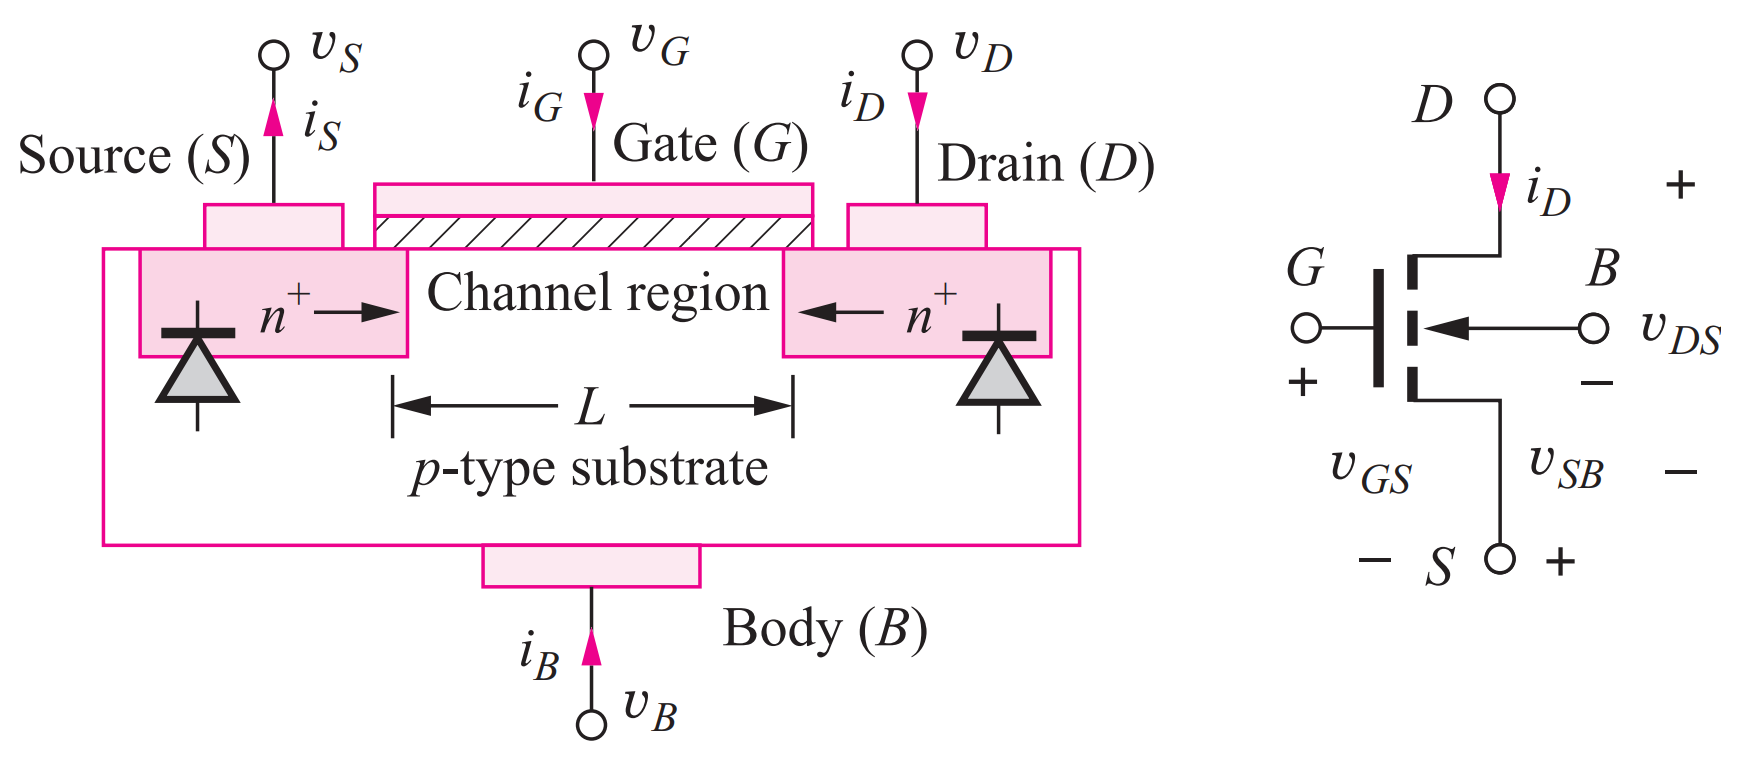
\includegraphics[width=0.65\linewidth]{img/nMoas.png}
    \caption{Transistore nMOS}
    
\end{figure}

\subsection{Funzionamento qualitativo}

Assumiamo ora di mettere $V_B = V_S = 0$ e $V_D = piccola$, e studiamo le tre situazioni:

\begin{itemize}
    \item $V_{GS}\footnote{$V_{GS}$ indica la tensione tra il gate e source che è la tensione che conta per formare la zona di inversione} = 0$ o comunque 	molto	minore	di	$V_T$\footnote{Tensione di soglia}

    \item $V_{GS} < V_T$
    \item $V_{GS} > V_T$ circa un corto circuito
\end{itemize}

\subsubsection{$V_{GS} << V_T$}

Innanzitutto troviamo una zona di carica spaziale intorno ai due terminali, e in questa condizione non è formata nessuna zona di inversione ma in ogni caso non può passare corrente perché non abbiamo cariche mobili all'interno del substrato che possono condurre.

Anche se al drain mettessimo una tensione positiva non scorrerebbe corrente.

\begin{figure}[htbp]
    \centering
    \includegraphics[width=0.4\linewidth]{img/V_gs<<Vt.png}
    \caption{Nessuna inversione}
    
\end{figure}

\subsubsection{$V_{GS} < V_T$}

Aumentando la tensione sul gate inizia a formarsi la regione di carica spaziale sotto il gate che si unisce a quella dei diodi (giunzione pn), ma continua a non passare nessuna correte. Questo perché la regione di svuotamento non fornisce cariche per la conduzione ma è costituita solo da ioni fissi.



\begin{figure}[htbp]
    \centering
    \includegraphics[width=0.4\linewidth]{img/V_gs<Vt.png}
    \caption{Giunzione pn}
    
\end{figure}

\subsubsection{$V_{GS} > V_T$}
Quando la tensione sul gate raggiunge e supera la tensione di sogli $V_T$ ecco che si forma un canale di tipo n tra le sue regioni n+, un canale di elettroni mobili.

Ora se sul drain avessimo una tensione superiore del source ecco che potrebbe passare una corrente. Infatti la corrente dipende sia da $V_{GS}$, il quale determina il canale (quanti elettroni liberi) e da $V_D$.

\begin{figure}[htbp]
    \centering
    \includegraphics[width=0.4\linewidth]{img/V_gs>VT.png}
    \caption{Canale di elettroni}    
\end{figure}

\paragraph{Drain e Source}

Come si fa a distinguere il drain dal source? Teoricamente il transistore è un dispositivo a quattro terminali simmetrico dunque possiamo deciderli noi quale è l'uno e quale è l'altro, nei circuiti integrati funziona proprio così. Però in commercio i transistori (i componenti discreti) hanno solitamente tre terminali, questo significa che il costruttore ha deciso per noi chi è chi collegando un terminale con il substrato il quale è il \textbf{source}.


\subsection{Calcoliamo il valore della corrente di drain $I_D$}

Vogliamo calcolare la corrente che scorre tra drain e source in funzione della tensione sul gate e della tensione sul drain, supponendo di mettere il source a massa.

\paragraph{}
Per prima cosa possiamo calcolare la corrente del gate $I_G$, non essendo collegato a nulla le cariche non possono scorrere anche se il gate si trova alla stessa tensione del generatore $V_{GS}$, quindi $I_G = 0 A$. Si comporta come un condensatore carico.

Solo all'inizio scorre un po' di corrente fino a che il gate si carica.
\paragraph{}

Supponiamo che $V_{DS}$ si positiva ma piccola e che $V_{GS} > V_T$.

La tensione $v(x)$ dentro il canale non è costante ma varierà lungo tutto il canale, in prima approssimazione possiamo affermare che vada linearmente da $V_S = 0$ a $V_D = V_{DS}$. Inoltre la corrente di drain è sostanzialmente una corrente  di drift.

\begin{figure}[htbp]
    \centering
    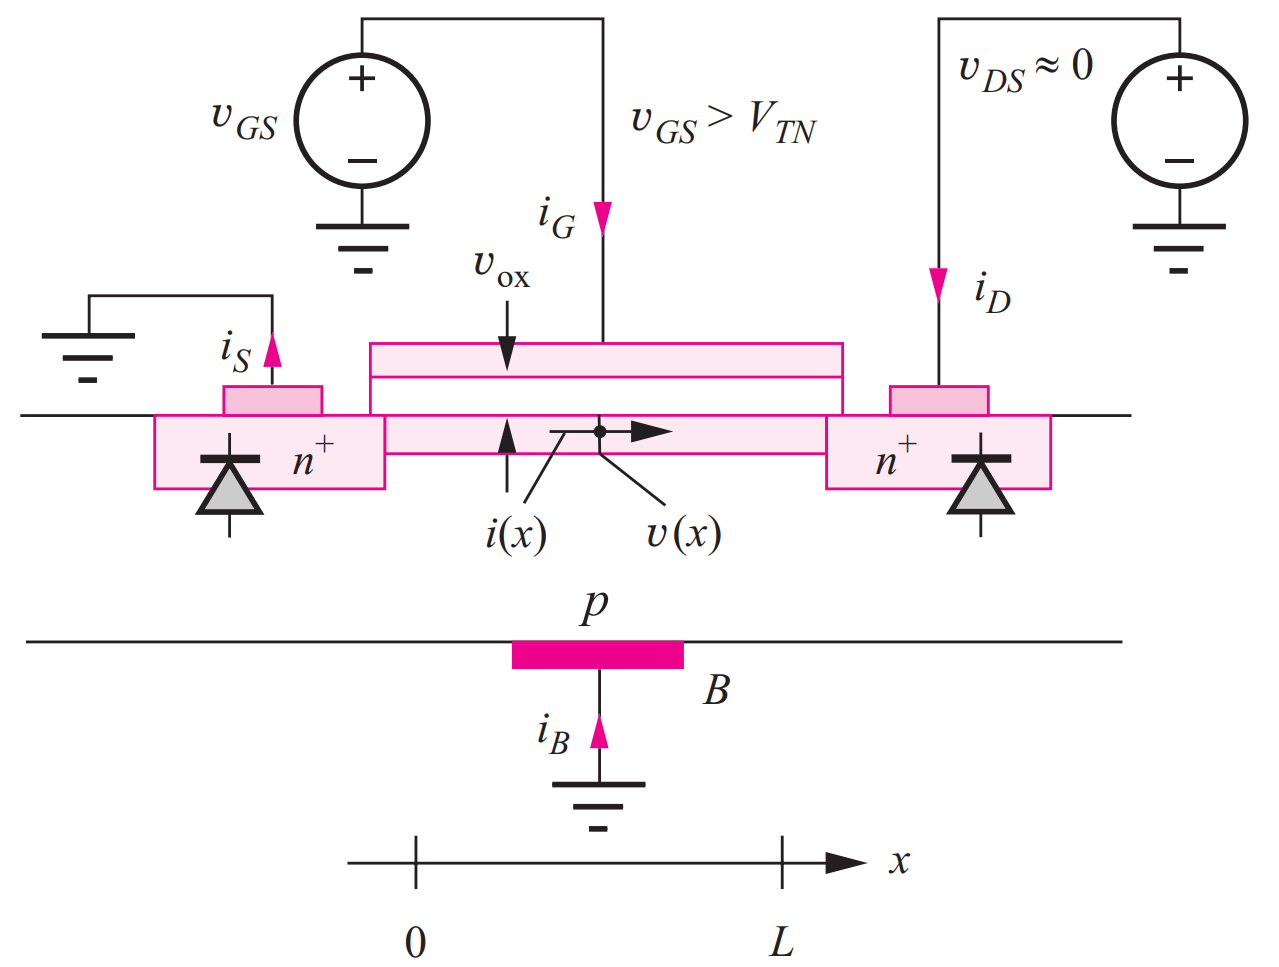
\includegraphics[width=0.4\linewidth]{img/corrente_drain.png}
    \caption{Corrente di drain}
    \label{fig:corrnte_srainnee}
\end{figure}


\paragraph{Carica nel canale}
Quanto vale la corrente di drift? Essa dipende dal campo elettrico, dalla mobilità, dalla velocità e dalla carica.

La	carica	presente	in	ogni	punto	del	canale	dipende	dalla	
tensione	sul	dielettrico,	come	in	un	condensatore.

\paragraph{Carica per unità di lunghezza}

\begin{equation}
    Q' = -WC_{ox}^{''}(v_{ox}-V_T)
\end{equation}

dove:

\begin{itemize}
    \item $C_{ox}^{''} = \frac{\varepsilon_{ox}}{T_{ox}}$, $\varepsilon_{OX}$ permittività dell'ossido e $T_{ox}$ è il suo spessore
    \item $v_{ox}(x) = V_{GS}-v_x$, $v_x$ è la tensione nel canale.
\end{itemize}

$v_{ox}\,$ deve	essere	maggiore di $V_T$ perché ci sia lo strato di inversione su tutto il canale e dunque cariche libere; $WC_{ox}^{''}$ capacità per unità di lunghezza; $v_{ox}-V_T$ tensione dell'ossido sottratta alla tensione soglia ovvero elimina il contributo degli ioni negativi fissi i quali non concorrono a creare una corrente.

La tensione sull'ossido varia lungo il canale, se in un condensatore formato da piastre metalliche ogni punto è equipotenziale, in questo caso nel semiconduttore questo non accade, quindi pure la quantità di carica non sarà costante, la differenza di potenziale sarà più alta tra source e gate a sinistra che tra drain e gate a destra Fig. \ref{fig:corrnte_srainnee}.

\newpage
\subsubsection{Corrente}
La corrente come al solito è data da:

\begin{equation}
    I(x) = Q'(x)s_x(x)\qquad \text{$s_x(x)$ velocità	delle	cariche	dovuta	al	campo	elettrico}
\end{equation}

\begin{equation}
    I(x) = -WC_{ox}^{''}(v_{ox}-V_T)(-\mu_nE_x)
\end{equation}

Ricordando il campo elettrico:

\begin{equation*}
    \vec{Ex} = -\frac{dv(x)}{dx}
\end{equation*}

Sostituendo tutto otteniamo:
\begin{equation}
    I(x) = -\mu_nWC_{ox}^{''}(V_{GS}-v_{ox}-V_T)\frac{dv(x)}{dx}
\end{equation}

Integrando lungo x:

\begin{itemize}
    \item per x = 0, v(0) = $V_S = 0$
    \item per x = L, v(L) = $V_{DS}$
    \item i(x) = $I_D$, la corrente non varia perché non ci sono altri percorsi alternativi
\end{itemize}

\begin{equation}
    \int_0^Li(x) dx = \int_0^L-\mu_nWC_{ox}^{''}(V_{GS}-v_{ox}-V_T)dv(x)
\end{equation}

Risolvendo l'integrale:

\begin{equation*}
    I_D\cdot L = \mu_nWC_{ox}^{''}(V_{GS}-V_T-\frac{V_{DS}}{2})V_{DS}
\end{equation*}
\begin{equation}
    I_D = \mu_n\frac{W}{L}C_{ox}^{''}(V_{GS}-V_T-\frac{V_{DS}}{2})V_{DS}
    \label{equazione_zona_triodo}
\end{equation}

Da notare che la corrente dipende dal rapporto di forma del transistore: $\frac{W}{L}$, in particolare quando è largo rispetto alla lunghezza. W grande corrente grande, W piccolo corrente piccola.

La corrente dipende dalla $V_{DS}$ in quanto è la "forza motrice" delle cariche e da $V_{GS}$ che mette a disposizioni gli elettroni per il passaggio di carica. Notiamo qui che la corrente dipende in modo \textbf{quadratico} con $V_{DS}$.

Valida	solo	se	la	tensione sull'ossido	è	superiore	alla soglia	VT in	ogni	punto:

\begin{itemize}
    \item $v_{ox} \geq V_T$
    \item $V_{GS} - v_{ox} \geq V_T$, $v_{ox}$ è	più	grande	al	drain
\end{itemize}

\paragraph{In particolare:}
\begin{itemize}
    \item $V_{GS} - V_{DS} \geq V_T$
    \item $V_{DS} \leq V_{GS} - V_T$
    \item $V_{GS} \geq V_{DS} + V_T$
\end{itemize}

Analizzando l'ultima disequazione: Perché  ci sia il canale, sicuramente ci deve essere una tensione $V_T$, in più aggiungiamo una tensione sul drain, ne risulta che la tensione gate-source deve essere maggiore di una VT rispetto alla tensione del drain.


\newpage
\section{Regione	lineare, ohmica	o	triodo}
Questa regione, che varia quadraticamente, viene chiamata lineare o triodo, la formula della corrente può essere riscritta in modo più compatto utilizzando la transconduttanza  ($K_N' = \mu_nC_{ox}^{''}$) che dipende dalla tecnologia (parametro tecnologico), la mobilità dei portatori dipende dal silicio e la capacità che dipende dal fattore geometrico, quale lo spessore, dell'ossido, dunque dipende da chi ve lo produce.

Talvolta nella transconduttanza viene anche inserito il rapporto tra larghezza e lunghezza: $K_N = \mu_nC_{ox}^{''}\frac{W}{L}$.

\begin{equation*}
    I_D = K_n\biggl(V_{GS}-V_T-\frac{V_{DS}}{2}\biggl)V_{DS}
\end{equation*}

\begin{equation}
    I_D = K_n\biggl((V_{GS}-V_T)V_{DS}-\frac{V_{DS}^2}{2}\biggl)
    \label{corrente_drain_formula}
\end{equation}


\paragraph{Esempio:} Calcoliamo il valore di $K_n'$ per un transistore con
\begin{itemize}
    \item $\mu_n = 500\,cm^2/Vs$ mobilità \footnote{Notiamo che la mobilità ha un valore molto più basso rispetto ai $1350\,cm^2/Vs$, questo è dovuto al fatto che le cariche si muovono sulla superficie che è a contatto con l'ossido.}
    \item $T_{os} = 25\,nm$ spessore dell'ossido 
\end{itemize}

\begin{equation*}
    K_n' = \mu_n\frac{\varepsilon_{ox}}{T_{ox}} = 500\cdot3.9\cdot8.854\cdot10^{-14}/25 = 69.1\,\mu A/V^2
\end{equation*}

\subsection{Se $V_{DS}$ è piccola}
Si chiama zona lineare perché se $V_{DS}$ è piccola la formula non compare il termine $V_{DS}^2$ e dunque il transistore si comporta come una resistenza \footnote{I = G$\cdot$V, dove G è la conduttanza $G=1/R$} (da cui anche zona ohmica) il cui valore può essere controllato da $V_{GS}$, quindi il modello diventa lineare:

\begin{equation}
    I_D = K_n(V_{GS}-V_{T})V_{DS}
\end{equation}

E per calcolare la resistenza equivalente basta fare il reciproco della conduttanza G:

\begin{equation}
    R_{on} = \frac{1}{K_n(V_{GS}-V_{T})}
\end{equation}

\begin{figure}[htbp]
    \centering
    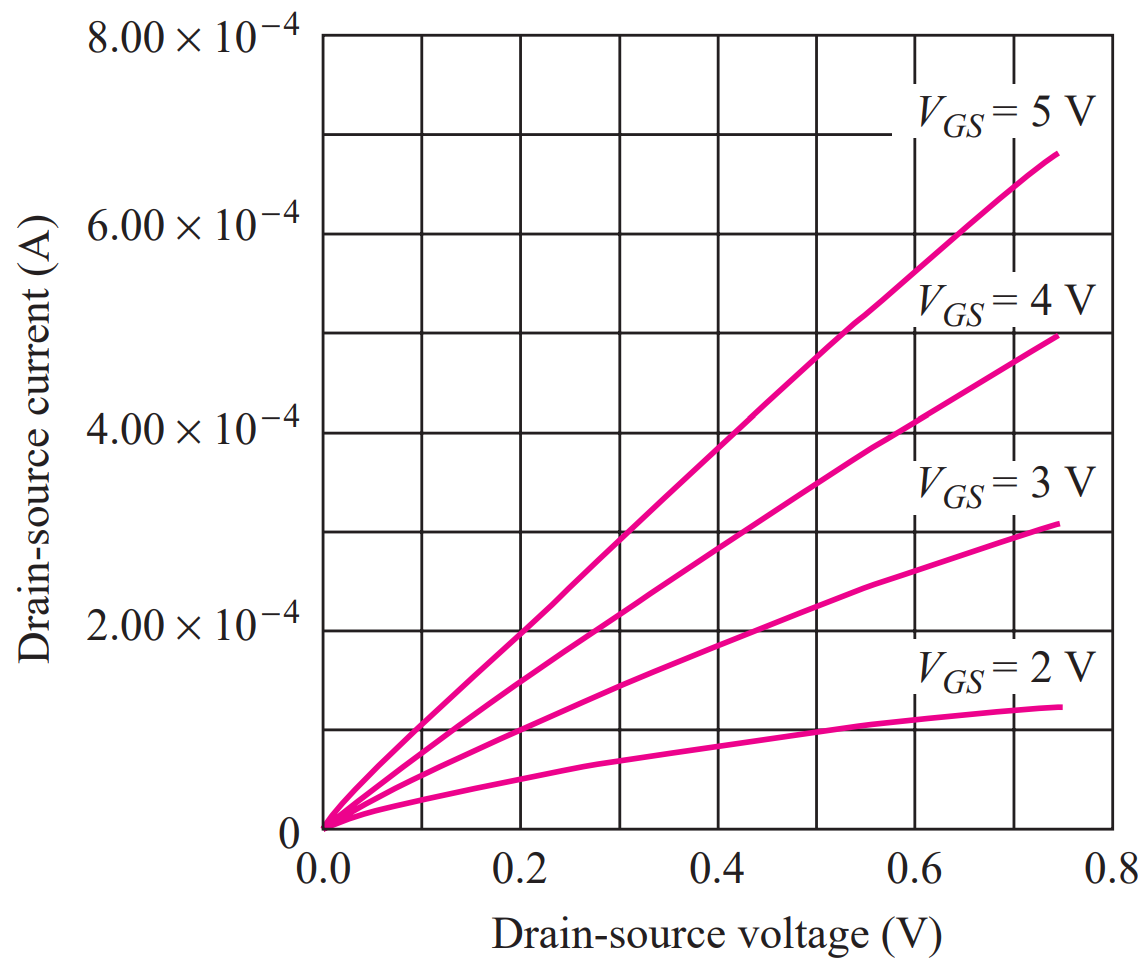
\includegraphics[width=0.4\linewidth]{img/regione_lineare.png}
    \caption{Regione lineare}
    
\end{figure}

Più si aumenta la $V_{GS}$ e più la resistenza risulterà bassa perché maggiori saranno i portatori sul canale.


\newpage
\section{Saturazione}
Il modello visto fino ad ora è valido fin tanto che:

% \begin{wrapfigure}{r}{0.6\textwidth} %this figure will be at the right
%     \centering
%     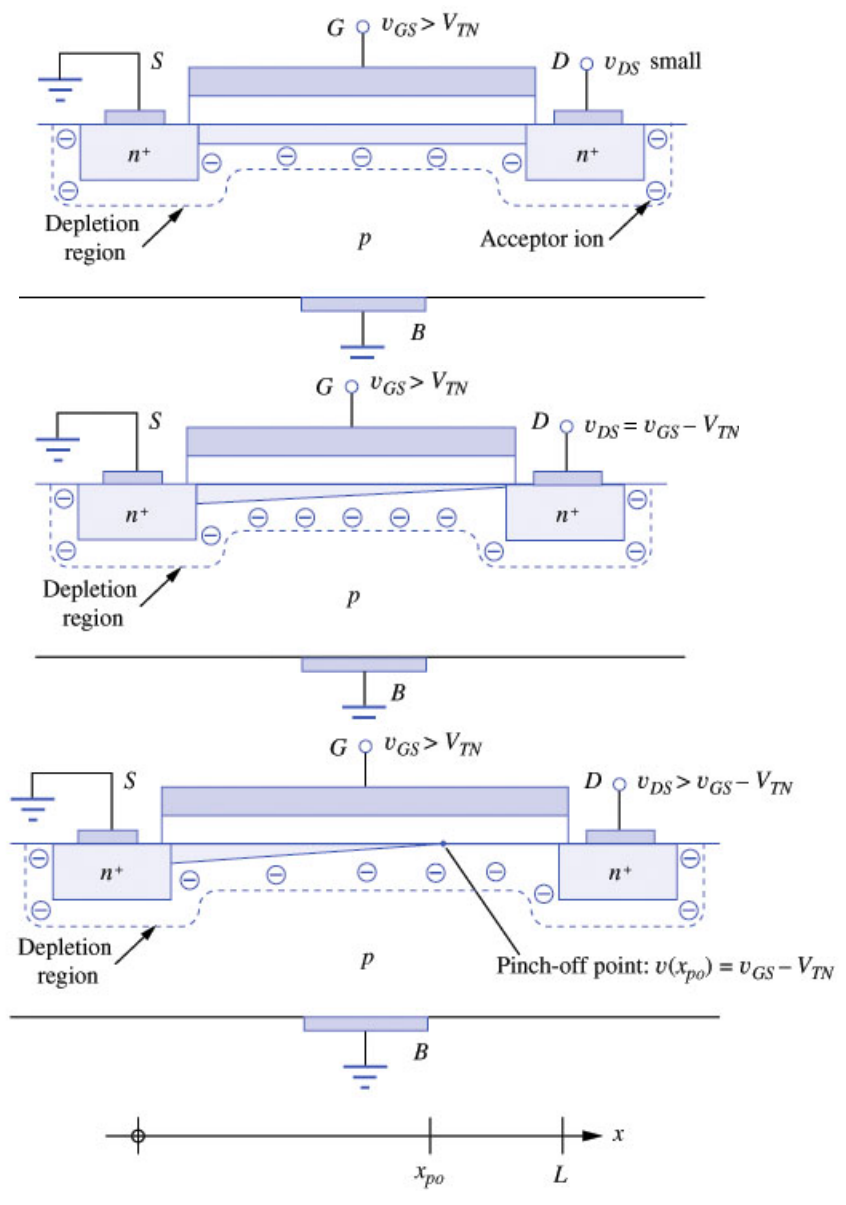
\includegraphics[width=1\linewidth]{img/image.png}
% \end{wrapfigure}


\begin{itemize}
    \item $V_{GS} \geq V_{DS} + V_{T}$
    \item La corrente $I_D$ aumenta in modo quadratico con $V_{DS}$.
\end{itemize}

\begin{figure}[htbp]
    \centering
    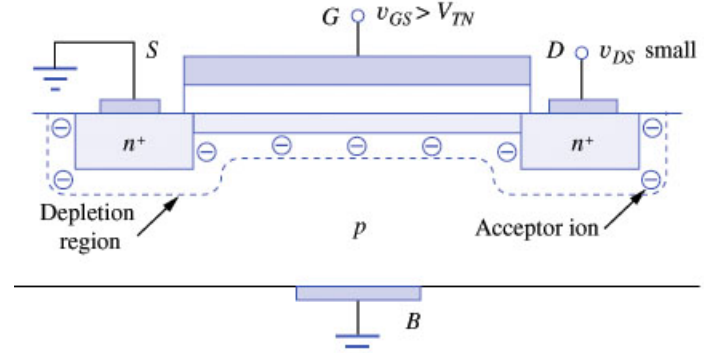
\includegraphics[width=0.45\linewidth]{img/berkley1.png}     
\end{figure}

Con l'aumento di $V_{DS}$ il canale si assottiglia verso il drain fino a scomparire per 
\begin{itemize}
    \item $V_{DS} = V_{GS} - V_{T}$
\end{itemize}

\begin{figure}[htbp]
    \centering
    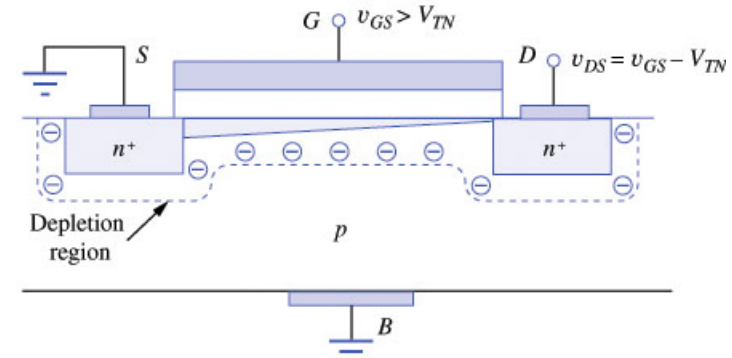
\includegraphics[width=0.45\linewidth]{img/berkley2.png}   
    
\end{figure}

Con ulteriori aumenti di $V_{DS}$ lo stato di inversione diventa nullo al drain e la corrente, non aumentando più, satura.
Quindi in prima approssimazione possiamo affermare che la corrente diventa costante, ma vedremo che non è del tutto così, leggermente aumenterà in quanto alla relazione: $E_x = -\frac{dV(x)}{dx}$, essendo che la lunghezza del canale diminuisce, aumenterà la tensione.

\begin{itemize}
    \item $V_{DS} \geq V_{GS} - V_{T}$
\end{itemize}

\begin{figure}[htbp]
    \centering
    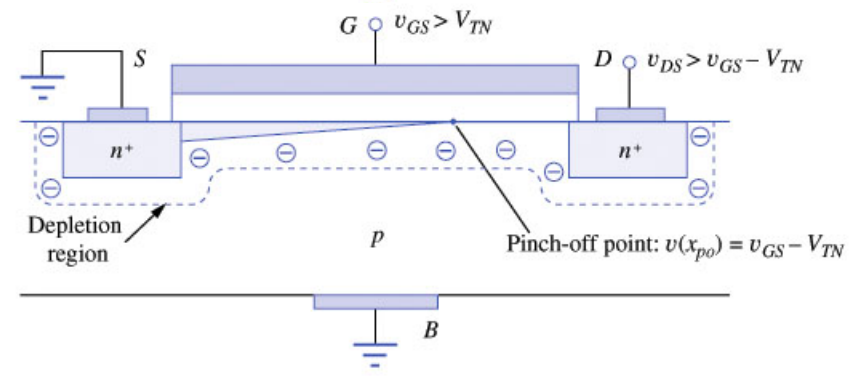
\includegraphics[width=0.45\linewidth]{img/berkley3.png}    
    
\end{figure}

\newpage
\subsection{E quanto satura?}
La corrente satura negli ultimi due casi, in particolare inizia a saturare dal valore per cui: $V_{DS} = V_{GS} - V_{T}$. E la corrente di saturazione sarà data da:

\begin{equation*}
    I_D = K_n'\frac{W}{L}\biggl(V_{GS} - V_T - \frac{V_{GS}-V_T}{2}\biggl)\big(V_{GS} - V_T\big)
\end{equation*}

\begin{equation}
    I_D = \frac{K_n'}{2}\frac{W}{L}\biggl(V_{GS} - V_T \biggl)^2
    \label{Equazione_corrente_pinch_off}
\end{equation}

Quindi vediamo subito che rispetto alla corrente di drain, Formula \ref{corrente_drain_formula}, la corrente è \textbf{indipendente} da $V_{DS}$.

La formula sopra riportata è valida per $V_{DS} \geq V_{DSAT} = V_{GS} - V_T$. La tensione $V_{DSAT}$ è chiamata tensione di \textbf{saturazione} o di \textbf{pinch-off}.

\begin{figure}[htbp]
    \centering
    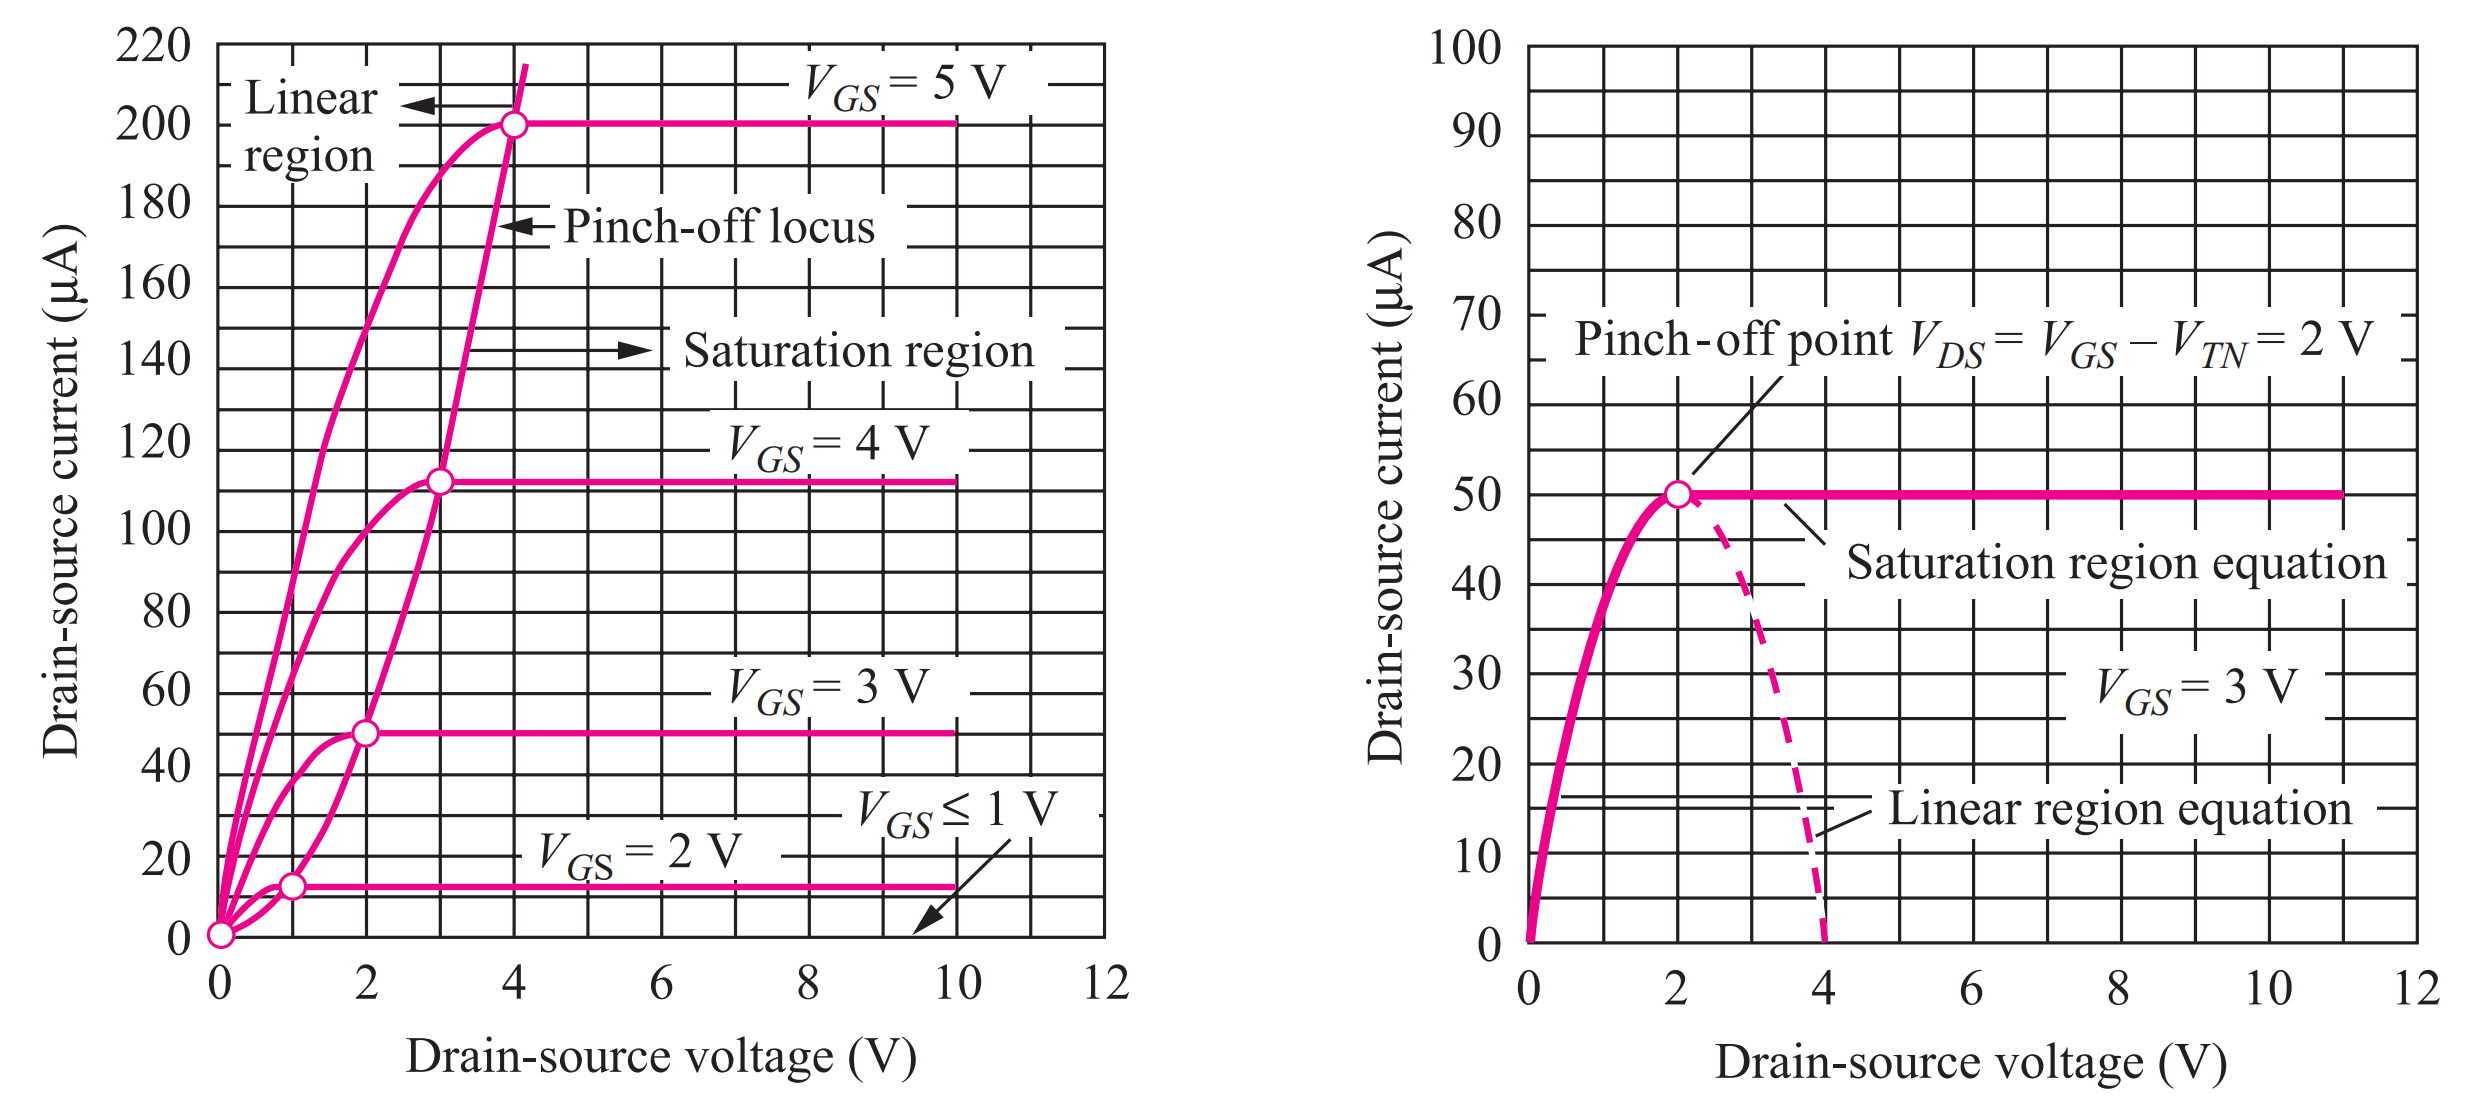
\includegraphics[width=0.9\linewidth]{img/pinch_off.png}
    \caption{Relazione corrente in funzione della tensione al drain}    
\end{figure}

 Osservando questo grafico troviamo dunque tre casi:

 \begin{itemize}
     \item $I_{DS} = 0A$
     \begin{itemize}
         \item Questo è il caso più semplice perché significa che $V_{GS} \leq V_T$
     \end{itemize}
     
    \item $V_{GS} \geq V_{DS} + V_T$
     \begin{itemize}
         \item parte del grafico che si forma una parabola rivolta verso il basso
         \item ci troviamo nella zona lineare
     \end{itemize}

     \item $ V_{DS} \geq V_{GS} - V_T$
     \begin{itemize}
         \item parte del grafico che si forma una retta
         \item ci troviamo nella zona di saturazione
     \end{itemize}     
 \end{itemize}

\paragraph{Esempio:} Supponiamo 

\begin{itemize}
    \item $V_T = 1V$
    \item $V_{GS} = 5V$
    \item $V_{DS} = 10V$
    \item $K_{n}^ = 40 \mu_A/V^2$
    \item $L = 0.35 \mu m, \quad W = 8.75 \mu m$
\end{itemize}

Per trovare \textbf{$I_D$} intanto dobbiamo capire in che regione ci troviamo utilizzando le disequazioni viste in precedenza.
In questo caso vediamo subito che siamo nella regione di saturazione e dunque possiamo applicare la relativa Formula \ref{Equazione_corrente_pinch_off} e sostituendo tutti i dati otterremmo $8 mA$.

 Da notare il rapporto di forma $W:L = 25:1$


\section{Modulazione di lunghezza di canale}
Abbiamo detto che all'aumentare di $V_{DS}$ la lunghezza del canale L effettiva diventa più piccola con la conseguenza che la corrente $I_D$ aumenta.

Normalmente nei circuiti ad alte prestazioni si vuole tenere una corrente elevata per andare più velocemente ma ovviamente ciò comporta un aumento di calore e una diminuzione della carica della batteria.

Per tener traccia di questo aumento nella formula vista in precedenza si aggiunge una costante moltiplicativa $\lambda$ chiamata parametro di modulazione di lunghezza del canale.

Normalmente $0 \leq \lambda \leq 0.2\,V^{-1}$


\begin{equation}
    I_D = \frac{K_n'}{2}\frac{W}{L}\big(V_{GS} - V_T \big)^2\big(1+\lambda V_{DS}\big)
    \label{Equazione_corrente_pinch_off_con_lambda}
\end{equation}

\begin{figure}[htbp]
    \centering
    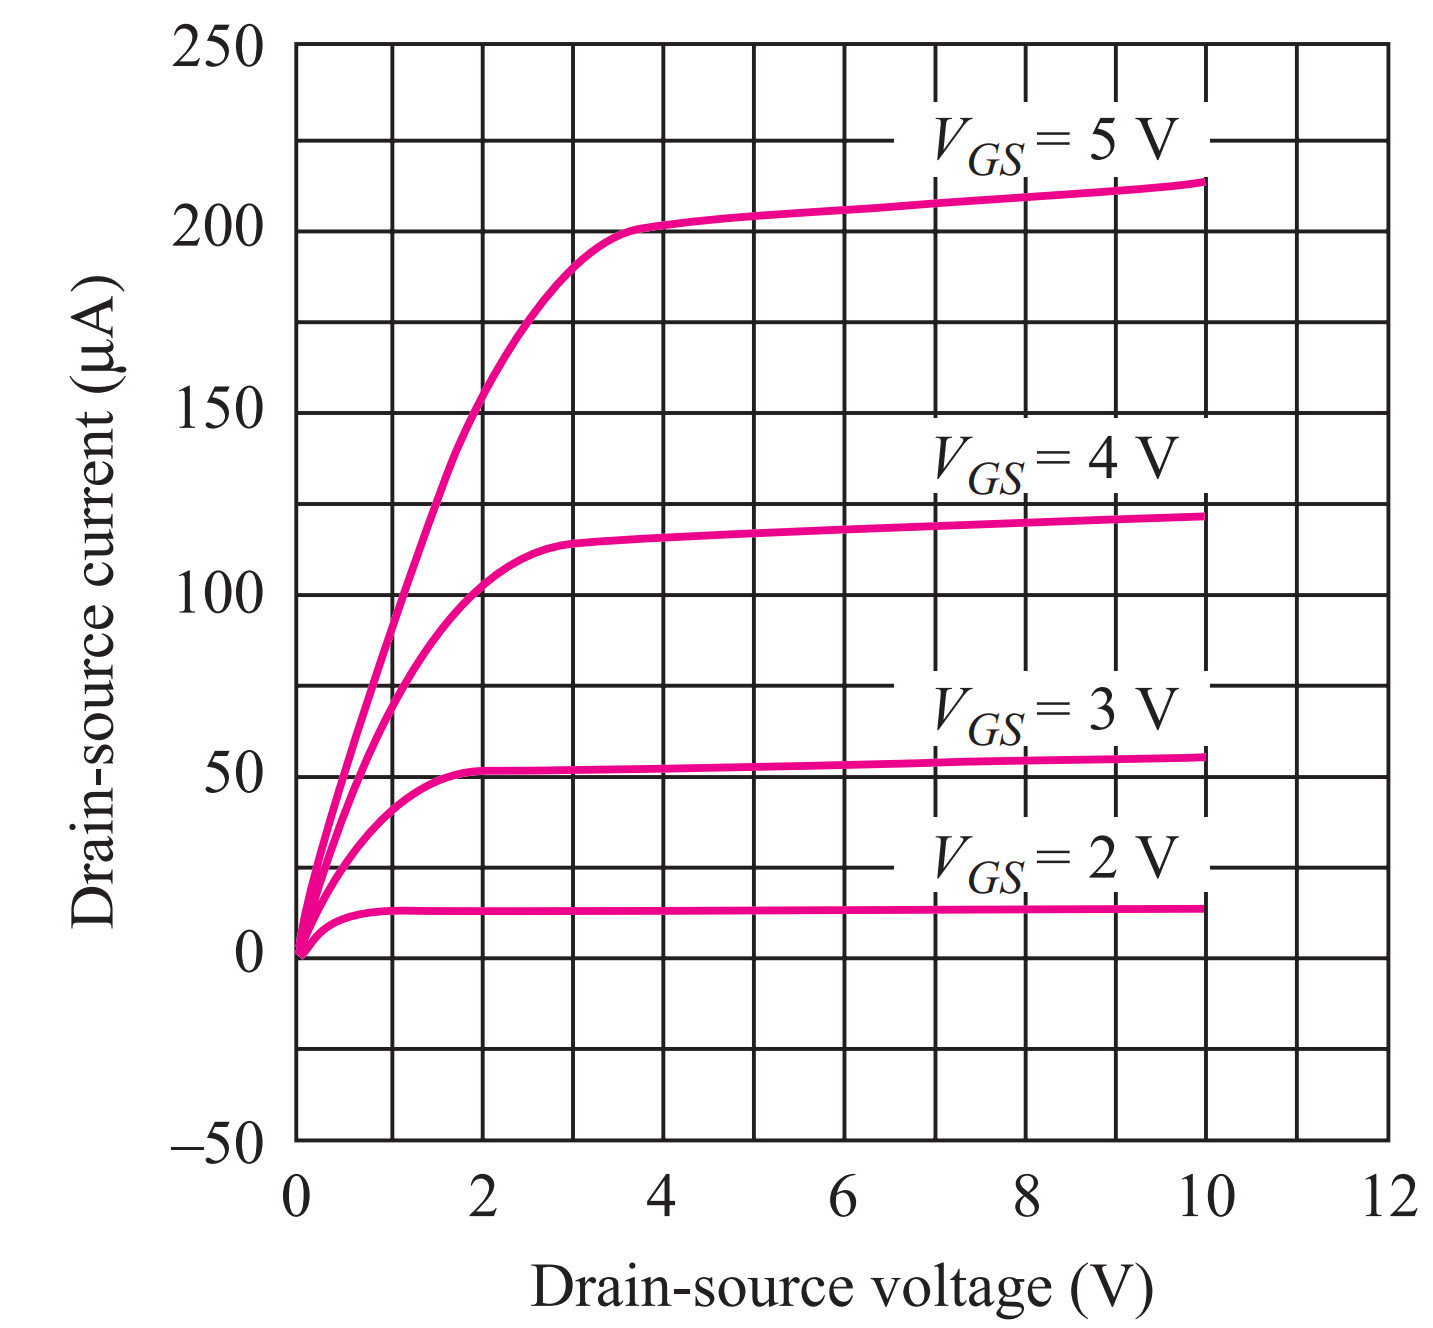
\includegraphics[width=0.4\linewidth]{img/lamda_modulazioneLungCanale.png}  
    
\end{figure}


\section{Modello matematico del transistore nMOS}

\subsubsection{Transconduttanza}

\begin{equation*}
    K_n = K_n'\frac{W}{L}\qquad\qquad K_n' = \mu_nC_{ox}''
\end{equation*}

\subsubsection{Zona triodo}
\begin{equation*}
    I_D = K_n\biggl(V_{GS}-V_{TN}-\frac{V_{DS}}{2}\biggl)V_{DS} \qquad\text{per } \qquad0\leq V_{TN} + \vds \leq \vgs
\end{equation*}

 \subsubsection{Regione di saturazione}
\begin{equation*}
    I_D = \frac{K_n}{2}\biggl(V_{GS}-V_{TN}\biggl)^2 \qquad\text{per } \qquad\vds \geq \vgs - V_{TN}
\end{equation*}

\begin{figure}[htbp]
    \centering
    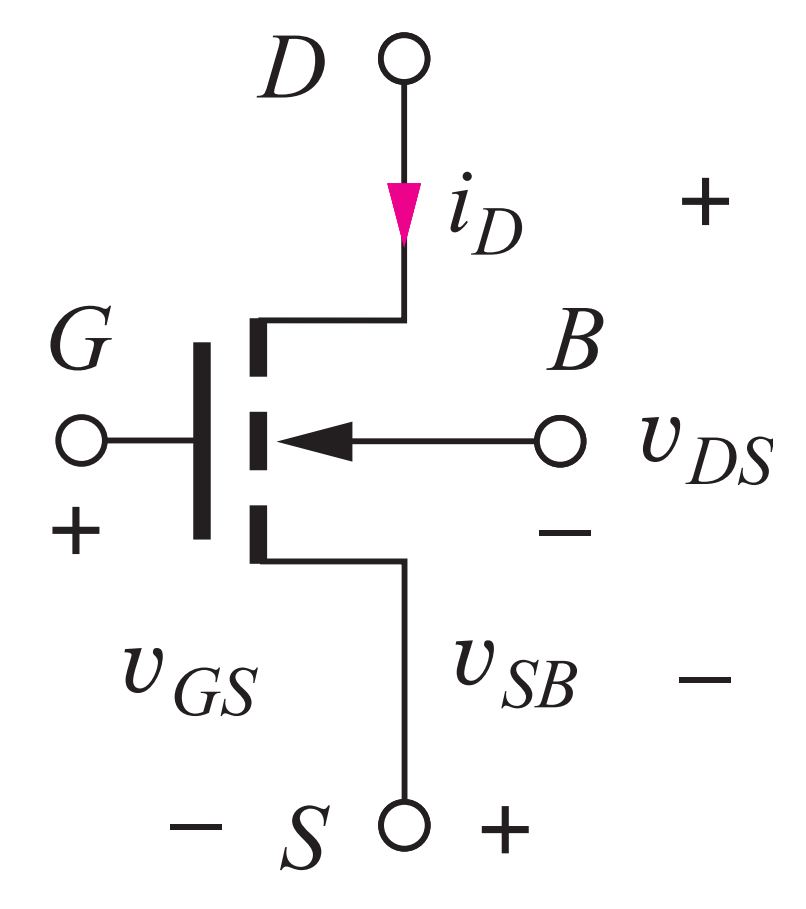
\includegraphics[width=0.2\linewidth]{img/nmossone.png}
    \caption{Transistore nMOS}
\end{figure}


\newpage
\section{Abbassare la tensione di soglia nel canale}
Arrivati a questo punto però ci potrebbe essere comodo abbassare questa tensione di soglia, il quale abbassamento farebbe in modo che il transistore possa condurre prima.

Vi sono due metodi: \textbf{Transistore	nMOS a	svuotamento} e \textbf{Effetto body}.


\section{Transistore	nMOS a	svuotamento}
Si potrebbe pensare di inserire direttamente il canale n direttamente nel substrato.

\begin{figure}[htbp]
    \centering
    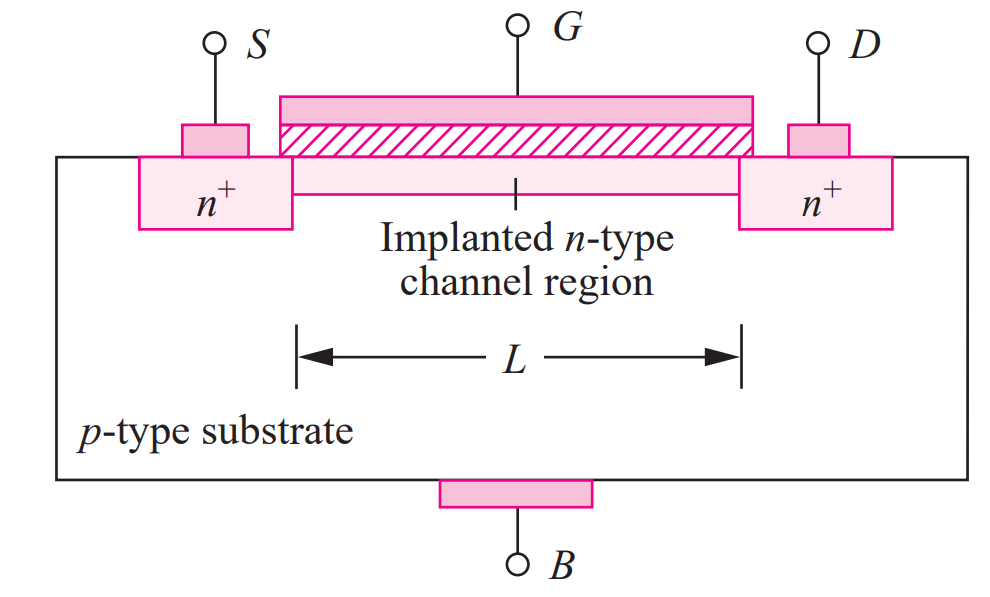
\includegraphics[width=0.4\linewidth]{img/n-type_impllanted.png}
    \caption{Transistore con canale di tipo n già inserito}
    
\end{figure}

Il canale dunque esiste già e il transistore	conduce	anche	per $\vgs = 0$, la tensione di soglia $\vt$ è  negativa, per il resto non cambia nulla.

Questo transistore prende il nome anche di transistore a \textbf{depletion mode}.


\subsection{Effetto body}

Altrimenti di potrebbe applicare una tensione al bulk $V_B$ diversa da zero per modificare la tensione di soglia

\begin{equation}
    \vt = V_{T0} + \gamma\big(\sqrt{V_{SB} + 2\phi_F} - \sqrt{2\phi_F}\big)
    \label{Equazione_effetto_body}
\end{equation}

dove
\begin{itemize}
    \item $V_{T0} $ valore di $\vt$ per $V_{SB} = 0$ , $\qquad -5\leq V_{T0} \leq 5$
    \item $\gamma $ parametro effetto body, $\qquad 0\leq \gamma \leq 3$
    \item $2\phi_F$ potenziale di superficie, $ \qquad 0.3 \leq 2\phi_F \leq 1$
\end{itemize}

\newpage
\section{Transistori pMOS}
In	modo	simmetrico,	si	può	realizzare	un	transistore	su	substrato	di	tipo	n,	con	source	e	drain	p+. Funziona tutto in maniera duale: tensioni e correnti invertire, mobilità delle lacune inferiore.

Per ottenere delle tensioni negative, non utilizzate nei dispositivi elettronici, basta mettere il source alla tensione più alta presente nel circuito, prima era a massa, e di conseguenza tutte le altre tensioni saranno inferiori o al più uguali a $V_S$.


\begin{figure}[htbp]
    \centering
    \includegraphics[width=0.8\linewidth]{img/pMOS.png}
    \caption{Transistore pMOS}    
\end{figure}

\section{Modello matematico del pMOS}

\subsubsection{Transconduttanza}

\begin{equation*}
    K_p = K_p'\frac{W}{L}\qquad\qquad K_p' = \mu_pC_{ox}''
\end{equation*}

\subsubsection{Zona triodo}
\begin{equation*}
    I_D = K_p\biggl(V_{GS}-V_{TP}-\frac{V_{DS}}{2}\biggl)V_{DS} \qquad\text{per } \qquad0\leq |\vds|\leq |\vgs - V_{TP}|
\end{equation*}

 \subsubsection{Regione di saturazione}
\begin{equation*}
    I_D = \frac{K_p}{2}\biggl(V_{GS}-V_{TP}\biggl)^2 \qquad\text{per } \qquad |\vds| \geq |\vgs - V_{TP}|
\end{equation*}

\begin{figure}[htbp]
    \centering
    \includegraphics[width=0.27\linewidth]{img/p_mos.png}
    \caption{Transistore pMOS}    
\end{figure}


\section{Riassunto}

Nel transistore MOSFET troviamo quattro terminali: 

\begin{itemize}
    \centering
    \item[] Gate \qquad \qquad Source \qquad \qquad Drain \qquad \qquad Body
\end{itemize}

e tre zone di funzionamento:

\begin{itemize}
    \item[] \textbf{Cut-off}: se $\vgs$ è sotto la tensione di voglia $\vt$, ciò non fa scorrere corrente tra $I_D$ tra drain e source
    \item[] \textbf{Triodo}: se $\vgs$ è sopra la tensione di soglia $\vt$ lungo tutto il canale, la corrente $I_D $ tra	drain	e	source	dipende	da	$\vgs$ e	da	$\vds$ secondo	la	legge	quadratica :
    \begin{itemize}
        \item[] \begin{equation*}
            I_D = K_n\biggl(V_{GS}-V_T-\frac{V_{DS}}{2}\biggl)V_{DS}\qquad \text{per} \qquad \vt \leq \vgs \geq \vds + \vt
        \end{equation*}
    \end{itemize}

    \item[] \textbf{Saturazione} se $\vgs$ è	sopra	la	tensione	di	soglia $\vt$ per	parte	
    del	canale,	la	corrente $I_D$ tra	drain	e	source	non	dipende	da $\vds$ e dipende da $\vgs$ secondo una legge quadratica:
    \begin{itemize}
        \item[] \begin{equation*}
                I_D = \frac{K_n}{2}\biggl(V_{GS} - V_T \biggl)^2\qquad \text{per} \qquad \vgs \leq \vds + \vt
        \end{equation*}
    \end{itemize}

\end{itemize}

\begin{figure}[htbp]
    \centering
    \includegraphics[width=0.45\linewidth]{img/recap.png}
    \caption{Caratteristica I-V}
    
\end{figure}

\newpage
\section{Modello di analisi}
Occorre	stabilire	la	regione	di	funzionamento	del	transistore	in	modo	da	applicare	la	formula	giusta. Se	difficile	da	dire	a	priori,	si	fanno	delle	ipotesi	e	poi	si	verifica	
che	i	risultati	siano	consistenti	con	le	ipotesi	(come	già	fatto	
per	i	diodi).

Spesso	si	faranno	delle	semplificazioni,	considerando	solo	il	
punto	di	inizio	e	di	fine	di	un	transitorio,	per	evitare	di	dover	
integrare	lungo	tutta	la	caratteristica.

\subsubsection{Circuiti digitali e amplificatori}

Per	circuiti	digitali	si	lavora	in	cut-off	(interruttore	aperto)	o	in	
regione	lineare	(interruttore	chiuso)

\subsubsection{Amplificatori}

Per	amplificatori	si	lavora	in	regione	di	saturazione	(generatore	
di	corrente	costante,	controllata	dalla	tensione	di	ingresso)

\paragraph{}
Bisogna fare attenzione che la $\vds$ dipende dal resto del circuito, infatti non 	è	imposta	direttamente	da	un
generatore	di	tensione ma dipende	dalla	corrente	di	drain.

\subsection{Calcolo con la retta di calcolo}

Dato il seguente circuito, formato da un singolo transistore con source a massa e gate e drain collegato ad un generatore di tensione.

Assumendo $\vt = 1V$ e $K_n = 220 \mu A/V^2$, trovare la corrente e la tensione tra drain e source.

$\vt$ è possibile trovarla facilmente. Basta mettersi in un punto di pinch-off e fare la differenza tra $\vgs$ e $\vds$.
\paragraph{}

\begin{figure}[htbp]
    \centering
    \includegraphics[width=0.3\linewidth]{img/calcolo_retta_carico.png}
    \caption{Circuito}    
\end{figure}

Per prima cosa dobbiamo trovare la retta di carico, ed utilizziamo l'equazione alla maglia del circuito a destra.

\begin{equation*}
    V_{DD} = I_DR + V_{DS}
\end{equation*}

Trovando che se la corrente è zero allora $\vds = \vgs$, e per trovare la massima corrente applicheremo la legge di Ohm tra la tensione $V_{DD}$ e la resistenza R.

Fatto ciò possiamo tracciare la retta di carico:

\begin{figure}[htbp]
    \centering
    \includegraphics[width=0.5\linewidth]{img/retta_carico_es.png}    
\end{figure}

\newpage

Ora vediamo a vari valori di $\vgs$ come si comporta.

\subsubsection{$\vgs \leq \vt$}

In questo caso vediamo che la corrente di drain è zero pure la corrente nella resistenza è zero

\paragraph{Troviamo M1}
Supponiamo ora di essere nella regione lineare e che $\vgs  = V_{DD}$, e che la tensione sia tutta sulla resistenza, dunque che $\vds$ sia piccola.  

Utilizzando la Formula \ref{equazione_zona_triodo} e l'equazione della retta di calcolo vista prima, mettendole a sistema possiamo trovare $\vds$ e $I_D$.

\begin{equation*}
    \vdd = K_n\biggl(\vgs - \vt - \frac{\vds}{2}\biggl)\vds R + \vds
\end{equation*}
\begin{equation*}
    \frac{K_nR}{2}\vds^2 - \big[1+K_nR(\vgs - \vt)\big]\vds + \vdd = 0
\end{equation*}
\begin{equation*}
    \vds = \frac{1+K_nR(\vgs - \vt)\pm \sqrt{\Big(1+K_nR(\vgs - \vt)\Big)^2 - 2K_nR\vdd} }{K_nR}
\end{equation*}
\begin{equation*}
    \vds = 0.65 V\qquad\qquad\qquad I_D = 525 \mu A
\end{equation*}

\subsubsection{Supponiamo di essere in saturazione}

Con $\vgs = 2.5V$ notiamo immediatamente dal grafico che ci troviamo in satura saturazione, proviamo dunque a calcolare come prima tensione e corrente, utilizzando sempre l'equazione della retta di calcolo e anche la Formula \ref{Equazione_corrente_pinch_off}.

\begin{equation*}
    \vdd = \frac{K_n}{2}(\vgs-\vt)^2R + \vds
\end{equation*}

\begin{equation}
    \vds = \vdd - \frac{K_n}{2}(\vgs-\vt)^2R
    \label{equazione_vds}
\end{equation}

\begin{equation*}
    \vds = 2.95 V\qquad\qquad\qquad I_D = 247.5\mu A
\end{equation*}

In questa zona il transistore ha una corrente costante e dunque si comporta come un generatore di corrente, e il valore della corrente lo controlliamo con la $\vgs$. Per piccole variazioni di $\vgs$, questo comporta il muoversi sulla retta di carico, causano grosse variazioni di $\vds$, funziona come un amplificatore.

\newpage
\subsection{Come determinare l'uscita $\vds$ in funzione dell'ingresso $\vgs$}

Vorremmo capire che relazione ci sia tra $\vds$ e $\vgs$, sicuramente dovremo vedere tutte le zone di funzionamento.

\subsubsection{Zona di Cut-off}

Partendo da $\vgs$ piccola, fintantoché questa è inferiore a $\vt$, corrente nel drain non ne scorre, non c'è caduta di potenziale sulla resistenza e l'uscita è 5V.

Questa zona infatti risulterà essere piatta.

\begin{figure}[htbp]
    \centering
    \includegraphics[width=0.4\linewidth]{img/IO_off.png}
    \caption{$\vgs < \vt$}    
\end{figure}

\subsubsection{Zona di amplificazione/saturazione}

Per ricavare la curva in questo caso basta assegnare dei valori a $\vgs$. Prendendo le equazioni della corrente e della retta di carico come fatto prima per ottenere la Formula \ref{equazione_vds} e sostituendoci $\vgs = \vds + \vt $ per trovare la zona di confine.

Questo vale fino a che $\vgs \leq \vds + \vt$

\begin{equation*}
    \vds = \frac{-2\pm \sqrt{4 + 8K_nRV_{DD}}}{2K_nR}
\end{equation*}

Una soluzione verrà negativa che ovviamente va scartata perché non c'è nessuna tensione negativa in questo circuito.

\begin{figure}[htbp]
    \centering
    \includegraphics[width=0.4\linewidth]{img/IO_ampl.png}
    \caption{$\vgs \leq \vds + \vt$}    
\end{figure}


\subsubsection{Zona di triodo}

Successivamente per $\vgs > \vds + \vt$ il transistore funziona in zona trodo.

\begin{equation*}
    V_{DS} = \frac{1+K_nR(\vgs - \vt ) \pm \sqrt{(1 + K_nR(\vgs - \vt))^2 - 2K_nR\vdd}  }{K_nR}
\end{equation*}

\begin{figure}[htbp]
    \centering
    \includegraphics[width=0.4\linewidth]{img/IO_triodo.png}
    \caption{$\vgs > \vds + \vt$}    
\end{figure}

Si può vedere che se l'ingresso è basso l'uscita è alta; se l'ingresso è alto l'uscita è bassa, anche perchè se fosse l'ingresso ad un altro transistore sarebbe sotto soglia (1V). Si comporta come invertitore logico.

Nella zona intermedia si comporta in modo differente: un piccolo cambiamento di $\vgs$, l'ingresso, comporta un grande cambiamento per l'uscita $\vds$. La derivata in valore assoluto è maggiore di 1.


\newpage
\section{Saturazione di velocità}
Come accennato in precedenza, all'aumentare del campo elettrico  i portatori raggiungeranno un limite di velocità, oltre ($\vec{E} > 10^5\,V/cm$) non aumentano più.

In maniera approssimata possiamo dire che $\vec{E} = \frac{\vds}{L}$, dunque aumentiamo il campo elettrico aumenta la corrente (perché aumenta la velocità dei portatori). Se la velocità satura, aumentando il campo elettrico ma la velocità non aumenta e nemmeno la corrente la quale diventa costante.
\paragraph{}
Una saturazione di velocità porta inevitabilmente ad una saturazione di corrente, non dovuta al fatto che non vi è più inversione ma è dovuta al fatto che i portatori non possono andare più velocemente. Si potrebbe arrivare prima in saturazione di velocità rispetto alla saturazione di pinch-off, questo dipende dalla lunghezza del canale.

Normalmente con le tecnologie moderne, siamo sempre in saturazione di velocità, e soprattutto vogliamo correnti elevate.

\paragraph{}

Dunque ad un	certo	punto,	pur	aumentando	$\vds$ e	quindi	il	campo elettrico	$\vec{E}$,	la	velocità	non	aumenta	più.

Supponiamo che la saturazione si raggiunga per $\vds = V_{SAT} = \vec{E}\cdot L$, la corrente non aumenta più in funzione a $\vds$.

\paragraph{Nota:}
Non	confondete	la	\textbf{regione	di	saturazione} con	la	\textbf{saturazione	di	velocità}.	
Si	può	avere	saturazione	di	velocità	in	zona	triodo,	o	non	avere	
saturazione	di	velocità	in	regione	di	saturazione!

Se	siamo	in	regione	di	saturazione	con	\textbf{saturazione	di	velocità},	la	
corrente	cresce	linearmente	con $\vgs$,	invece	che	quadraticamente!

\paragraph{Esempio: } si consideri $L = 1\mu m$, $100 nm$, $22 nm$, $5nm$. Troviamo a che valore di $\vds$ causa la saturazione di velocità:

\begin{itemize}
    \item[] $V_{SAT} = 10^{-4}\cdot10^5 = 10 V$
    \item[] $V_{SAT} = 10^{-5}\cdot10^5 = 1 V$
    \item[] $V_{SAT} = 22\cdot10^{-6}\cdot10^5 = 0.22 V$
    \item[] $V_{SAT} = 5\cdot10^{-7}\cdot10^5 = 0.05 V$
\end{itemize}

Se prendiamo in considerazione il secondo caso, è normale usare 1V nei circuiti, ma talvolta potremmo avere tensioni più alte come 1.8V e a quel punto saremo in saturazione di velocità.

Con $22nm$ siamo praticamente sempre in saturazione di velocità perché la tensione di alimentazione non è ancora arrivata ad essere 0.22V, ma non potrà mai essere sotto a 0.6 V perché il transistore ha una tensione di soglia e se si scende sotto ad essa non si può proprio accendere. Per ovviare a questo ci sono altri metodi.


\subsubsection{Saturazione di velocità}
La zona di saturazione è un limite che sotto al quale possiamo essere o in zona \textbf{triodo} o in nella regione di \textbf{pinch-off}.
L'espressione singola che riassume il tutto e la segiente:

\begin{equation}
    I_D = K_n\biggl(\vgs - \vt -\frac{V_{MIN}}{2}\biggl)V_{MIN}(1-\lambda\vds)
\end{equation}

dove $V_{MIN}:$

\begin{equation*}
    V_{MIN} = min((\vgs - \vt ), \vds, V_{SAT})
\end{equation*}

quindi il minimo tra, in ordine, saturazione, triodo e saturazione di velocità.

\begin{figure}[htbp]
    \centering
    \includegraphics[width=0.5\linewidth]{img/v_sat.png}
    \caption{Regione di saturazione}    
\end{figure}

\newpage
\subsection{Conduzione sotto soglia}
Abbiamo detto che per $\vgs < \vt$ la	corrente	di	drain	è	nulla. Ma	anche questa è	una	approssimazione,	infatti ci	sono	comunque	dei	portatori		e	ci	sono	le	correnti	inverse	dei	diodi. 

Se $V_{DS} > 0$ scorre una debole corrente, più	la	tensione	di	soglia	è	bassa,	più	è	alta	la	corrente	sotto	
soglia. Ciò può	diventare	significativa	quando	ci sono	miliardi	di	dispositivi!

\begin{figure}[htbp]
    \centering
    \includegraphics[width=0.5\linewidth]{img/corrente_sotto_soglia.png}
    \caption{Corrente sotto soglia, con $V_{DS}$ fissata}
    
\end{figure}


Inoltre tanto più bassa è la soglia del dispositivo, tanto più alta è la corrente sotto soglia. Sarebbe bello fare dei transistori con tensione di soglia molto piccola perché diminuirebbe l'assorbimento di potenza, ma ciò non è possibile perché conduce.

Alcuni circuiti basano il loro funzionamento proprio sul fatto che vi è questa corrente sotto soglia, ma ciò comporta che questi circuiti vadano bene se vogliamo costruite dispositivi non preformanti: il sensore di temperatura.
\paragraph{}
Ad alte prestazioni questa corrente sotto soglia comporta che il dispositivo consuma anche quando sta fermo, idealmente una porta consuma quando si deve scaricare e caricare, non quando sta ferma. Questo consumo non possiamo evitarlo il quale si attesta sull'ordine dei $mA$.








 \chapter{Invertitore Logico}
Come primo esempio di porta logica vediamo una delle porte più semplici: \textbf{l'invertitore}.

Quando la tensione in ingresso è piccola fornisce una tensione alta in uscita, e viceversa.

\section{Funzione di trasferimento e caratteristica}

\begin{itemize}
    \item $V_+$ e $V_-$ sono le tensioni di	alimentazione, $V_+$ alle volte è chiamata $\vdd$ (drain) e altre $v_{CC}$ (collettore) per i transistori bipolari.
    \item $V_H$ e $V_L$ sono i livelli alti e	bassi	della	tensione	di	uscita
\end{itemize}

\begin{figure}[htbp]
    \centering
    \includegraphics[width=0.75\linewidth]{img/inverter.png}
    \caption{Funzione ingresso/uscita e simbolo circuitale}    
\end{figure}

\subsection{Schema di base dell'invertitore}

Per ottenere il risultato che ci aspettiamo da un invertitore dobbiamo utilizzare due circuiti in modo tale da pilotare l'uscita verso il valore logico alto o basso, chiamati \textbf{pull-up} e \textbf{pull-down}.

\begin{itemize}
    \item[] La	rete	di	pull	down	porta	l’uscita	al	valore	basso;
    \item[] La	rete	di	pull	up	porta	l’uscita	al	valore	alto.
\end{itemize}

Dunque le tensioni in ingresso NON vengono usate per portare l'uscita al valore desiderato per solamente per attivare i due circuiti, è il circuito di pull-up/down che pilota l'uscita.

In questo modo la tensione in uscita tende verso il valore del circuito che "tira più forte".


\begin{figure}[htbp]
    \begin{minipage}[htbp]{0.5\textwidth}
    \centering
        \includegraphics[width=0.6\linewidth]{img/pull_u_d.png}   
    \end{minipage}
    \begin{minipage}[htbp]{0.5\textwidth}
    \centering

    \begin{tabular}{c|c c}
             & \textbf{Pull-up OFF} & \textbf{Pull-up ON} \\
             \hline
        \textbf{Pull-down OFF} & Z (float)\footnote{alta impedenza, l'uscita può mantenere il livello, scaricarsi o caricarsi anche rispetto alle condizioni circostanti dato il fenomeno del campo magnetico generato attorno al filo} & 1 \\
        
        \textbf{Pull-down ON} & 0 & Dipende\footnote{Il circuito è come un partitore di tensione, chi tira di più vince} \\
    \end{tabular}
    
    \end{minipage}
\end{figure}


% \begin{figure}[htbp]
%     \centering
%     \includegraphics[width=0.35\linewidth]{img/pull_u_d.png}    
    
% \end{figure}

% \begin{table}
% \centering
%     \begin{tabular}{|c|c|c|}
%         \hline
%              & \textbf{Pull-up OFF} & \textbf{Pull-up ON} \\
%         \hline
%         \textbf{Pull-down OFF} & Z (float)\footnote{alta impedenza, l'uscita può mantenere il livello, scaricarsi o caricarsi anche rispetto alle condizioni circostanti dato il fenomeno del campo magnetico generato attrono al filo} & 1 \\
%         \hline
%         \textbf{Pull-down ON} & 0 & Dipende\footnote{Il circuito è come un partitore di tensione, chi tira di più vince} \\
%         \hline
%     \end{tabular}
% \end{table}


\subsection{Interruttore	con	carico	resistivo}

Il modo di realizzare un invertitore è quello di creare dei cammini verso $\vdd$ e verso massa. L'inverter più semplice è quello denominato a \textbf{carico resistivo} costituito da una resistenza che collega sempre l'uscita a $\vdd$ con un impedenza diversa da zero la quale tira verso l'alto; e un circuito di pull-down realizzato con un transistore 	MOS, interruttore, che quando $v_i$ è bassa, 	l’interruttore	è	aperto (non tira verso massa) e l'uscita è alta, fase di \textbf{\textit{pull-up}}.


% In questo caso tanto è più grande è la resistenza, tanto più la corrente fa fatica a passare (circuito aperto) e quindi tanto è più alta la differenza di potenziale tra \vp e \vo.

% DA RIGARDARE QUESTA ILTIMA FRASE


\paragraph{}

Quando $v_i$ è	alta,	l’interruttore	è	chiuso,	e	l’uscita	è	connessa	a	
massa	dal	transistore, se quest'ultimo tira più forte di R, a massa, fase di \textit{pull down}.

\begin{figure}[htbp]
    \centering
    \includegraphics[width=0.55\linewidth]{img/interr_resist.png}
\end{figure}
\section{Caratteristica reale}
Ovviamente prima abbiamo visto un grafico dove si mostrava il comportamento ideale di questo circuito, in realtà l'andamento non sarà lineare. Agli estremi troveremo le zone che interessano ai circuiti elettronici digitali, i quali rappresentano 0 o 1, mentre della zona centrale è detta di \textbf{amplificazione}.

\begin{figure}[htbp]
    \centering
    \includegraphics[width=0.75\linewidth]{img/grafico_invert_resist.png}
    \caption{Caratteristica reale invertitore resistivo}    
\end{figure}


\newpage
\section{Margini di rumore}

Come posso definire il cambiamento dello stato? Una prima grossolana approssimazione potrebbe essere quella di dividere a metà, con una soglia, la tensione di alimentazione. Tutto quello che sta al di sopra lo possiamo considerare altro e quello che sta sotto basso.

Questo metodo però non porterebbe a risultati ottimali in quanto se un segnale è a ridosso della soglia, solo un po' di rumore porterebbe a far variare l'uscita.

\paragraph{}
Dunque una soluzione è quello di stare lontano dalla soglia e avere un\textbf{ margine di errore}. Come possiamo definirlo questo margine di errore?

Osservando quando nel grafico della caratteristica si incontrano i punti in cui la tangente alla curva tende al valore $-1$: le	tensioni	per	le	quali	la	tangente	vale	$-1$ discriminano	il	livello	alto	e	basso.

Questo perché possiamo discriminare le parti del circuito che si comportano come amplificazione, infatti nella zona centrale la derivata ha un numero in valore assoluto più grande di 1, quindi presenta un amplificazione.

Le zone più esterne invece, dove la tangente ha un valore $-1 < x < 0$, l'inverter attenuerà, in particolar modo se vi è del rumore ne riduce di molto la componente.  

\paragraph{Notazione: }

\begin{itemize}
    \item[$\blacktriangleright$]    \textbf{\vil} : tensione	massima	per	la	quale l’ingresso	è	considerato	basso;

    \item[$\blacktriangleright$] \textbf{\vih} : tensione	minima	per	la	quale l’ingresso	è	considerato	alto;

    \item[$\blacktriangleright$] \textbf{\vol}: valore estremo	di	uscita	per \vi = \vih;
    \item[$\blacktriangleright$] \textbf{\voh}: valore  estremo di uscita per \vi = \vil.
    \item[$\blacktriangleright$] \textbf{\vol}: valore estremo	di	uscita	per \vi = \vih;
    \item[]
    \item[$\blacktriangleright$] $NM_H = V_{OH} - V_{IH}$ 
    \item[$\blacktriangleright$] $NM_L = V_{IL} - V_{OL}$ 
\end{itemize}

La zona di mezzo, amplificazione, per questa tipologia di scopo e circuiti non si dovrà considerare.


\paragraph{}

Utilizzando più porte logiche, se l'ingresso abbiamo \vih, in uscita ci troviamo \vol, la quale a sua volta deve essere riconoscere come tensione bassa.

Dunque $V_{OL}$ deve essere inferiore alla massima tensione che l'inverte a valle riconosce come bassa che è \vil : \vol $\,\leq\,$ \vil, se verificata il circuito funziona.

Nel caso opposto avremo che: \voh $\,\geq\,$ \vih. 

\paragraph{}
Questa differenza è definita \textbf{Margine di rumore}.


\begin{figure}[htbp]
    \centering
    \includegraphics[width=0.45\linewidth]{img/cascata.png}    
    
\end{figure}

\newpage
\section{Obiettivi di progetto}
Ora dobbiamo progettare l'inverter in modo tale da renderlo migliore:

\begin{itemize}
    \item Minimizzare la regione indefinita, la caratteristica deve essere la più verticale possibile;
    \item Massimizzare i margini di rumore, dunque oltre al rumore nel circuito potremmo utilizzare componenti con tolleranze più grandi (processo meno preciso = costo minore);
    \item Dispositivo unidirezionale, l'uscita non deve influenzare l'ingresso; 
    \item I livello di I/O devono essere compatibili, ovvero margini di rumori positivi, se fossero negativi non potremmo costruire circuiti in casata;
    \item Massimizzare gli indici le prestazioni:
    \begin{itemize}
        \item Area più piccola possibile (costo minore);
        \item Minimizzare i consumi di potenza;
        \item Operare alla massima velocità;
    \end{itemize}
\end{itemize}

Normalmente gli indici di prestazione sono in conflitti tra di loro.

\section{Circuito invertitore nMOS}

Il circuito per realizzare un invertitore è uguale all'amplificatore utilizzato in zona non lineare.

\begin{figure}[htbp]
    \centering
    \includegraphics[width=0.35\linewidth]{img/calcolo_retta_carico.png}
    \caption{Circuito}    
\end{figure}

L'uscita la prendiamo attaccando un filo sul drain: $\vds = V_O$. A questo punto, al contrario dell'analisi, ora dobbiamo progettarlo con determinate prestazioni.

Messo per iscritto che utilizzeremo un inverter a carico resistivo e che la topologia sia quella in figura, dobbiamo scegliere: la dimensione di R e determinare il valore del rapporto $W/L$.

La L normalmente viene fissata con la tecnologia minima di produzione in quel momento (180 nm, 20 nm, ecc) si sceglie L più piccola in modo da portare più corrente possibile e minore dunque sarà la W e in generale il transistore diventa più piccolo.

\subsubsection{Obiettivo:}

\begin{itemize}
    \item[--] Rendere \vl $\,$ abbastanza bassa (sicuramente più bassa della $\vgs$) e \vh $\,$ = $\vdd$;
    \item[--] Minimizzare il consumo di potenza;
    \item [--] Massimizzare le prestazioni
\end{itemize}

\subsection{Scelta di \vl}

\textbf{La	tensione	di	uscita:}	deve	pilotare	la porta	logica	successiva, ovvero deve mettere in interdizione il gate del transistor successivo per metterlo in cut-off: \vl < $\vtn$, solitamente un valore appropriato si aggira tra 25\% e il 50\% di $\vtn$.

Nei transistori normalmente la $\vtn = 0.6V$, dunque possiamo scegliere una \vl $= 0.2V$, ovvero un terzo.
\paragraph{}
\textbf{Consumi di potenza:} Se il transistore è interdetto il generatore non eroga corrente (a meno quella per caricare il gate del transistor a valle), anche se la tensione rimane alta.

Quando \vi $\,$ è alta, scorre corrente e si consuma la batteria. Supponendo $\vdd = 2.5V$, vicino agli standard di oggi, scegliendo un consumo di potenza che ci aggrada, P = 0.2 mW, dettato dai parametri come: 

\begin{itemize}
    \item energia disponibile nella batteria;
    \item numero di porte logiche;
    \item la media di quante queste hanno l'uscita a zero;
    \item quanta potenza il sistema riesce a dissipare.
\end{itemize}

Partendo dal consumo totale ad esempio 0.2 W perché così so che la batteria mi dura due giorni, calcolando 2000 porte logiche di cui la metà a valore logico altro (potenza = 0), ottengo che ogni porta logica dovrà consumare 0.2 mW.


\subsection{Dimensionamento}
Come detto precedentemente supponiamo:
\begin{equation*}
    \vtn = 0.6V \qquad\qquad \vdd = 2.5V \qquad\qquad K_n' = 100\mu A/V^2
\end{equation*}

Per soddisfare i consumi di potenza:

\begin{equation*}
    \vdd \cdot I_D = 0.2 mW \qquad \longrightarrow \qquad I_D = 0.2 / 2.5 = 80 \mu A
\end{equation*}
Questa è la corrente che deve scorrere quando l'uscita è bassa (la porta consuma).

\paragraph{Calcolo R:}

\begin{equation*}
    I_D \cdot R = 2.5 - V_L = 2.5 - 0.2 \qquad \longrightarrow \qquad R = (2.5 - 0.2 ) / 0.00008 = 28.75 K\Omega
\end{equation*}
Si poteva anche ottenere grazie alla retta di carico, supponendo di avere un transistore discreto.

\paragraph{Calcolo il rapporto di forma W/L:}

\begin{equation*}
    V_i = \vgs = V_h = 2.5 V \text{,  } \qquad \vds = 0.2V
\end{equation*}

Trovandoci in zona triodo ($\vgs\,$ molto alta, $\vds\,$piccola, la tensione di soglia è 0.6 V, quindi $0.2 + 0.6 = 0.8V$ la $\vgs$ è molto più alta e dunque siamo in zona triodo) possiamo utilizzare la formula della zona triodo per trovare il rapporto W/L:

\begin{equation*}
    \frac{W}{L} = \frac{80 \mu A}{100 \frac{\mu A}{V^2} (2.5-0.6-\frac{0.2}{2})0.2} = 2.22 = \frac{2.22}{1}
\end{equation*}

Ora abbiamo tutti le dimensioni dei componenti. 

Non abbiamo considerato in questo caso le tempistiche. Queste ultime dipendono da quanto veloce la resistenza riesca a caricare il/i condensatore/i (gate) a valle.

Più piccola sarà R  più passa corrente e più verrà caricato in fretta il gate, per calcolare il tempo dobbiamo considerare il circuito come se fosse un RC, e con $\tau = RC$ ci possiamo ricavare quanto tempo impiega a caricarsi e scaricarsi.
\paragraph{}
Scegliendo una R piccola però significa che, si andremo più veloci, ma stiamo consumando anche più corrente. Vi è sempre lo scontro prestazioni e consumi.


\subsection{Calcoliamo i margini di rumore: \vil $\,$ e \voh}
Quando \vi $\,$ = $\vgs$ è piccola, ma maggiore della tensione di soglia, e \vo $\,$ = $\vds$ è grande ci troviamo sicuramente in \textbf{saturazione}.

Utilizzando la corrente di drain e il valore dell'uscita \vo = $\vdd - I_DR$, otteniamo:

\begin{equation*}
    V_o = V_{DD} - \frac{K_n}{2}(V_{GS}-V_{TN})^2 R
\end{equation*}

Cerchiamo dunque quando la tangente vale $-1$: la si ottiene facendo il rapporto tra la derivata in uscita e la derivata in ingresso

\begin{equation*}
    \frac{dV_o}{dV_{GS}} = - K_n(V_{GS}-V_{TN})R = -1
\end{equation*}

\begin{equation*}
    V_{IL} = V_{GS} = V_{TN} + \frac{1}{K_nR}
\end{equation*}

\begin{equation*}
    V_{OH} = V_{DD} - \frac{1}{2K_nR}
\end{equation*}


\begin{figure}[htbp]
    \centering
    \includegraphics[width=0.5\linewidth]{img/plot_.png}
    
    
\end{figure}

Per il valore logico alto, quando \vi $\,$= $\vgs$ è grande \vo $\,$= $\vds$ è piccola siamo in zona triodo. Come prima dobbiamo sempre derivare e uguagliare a -1, in questo caso la derivata risulterà più complicata, infatti risulta più semplice assumere che: $\frac{dV_o}{dV_{GS}} = \frac{dV_{GS}}{dV_o}^{-1}$

Il risultato diverrà:

\begin{equation*}
    V_O= \vdd - K_n\Biggl(\vgs- \vtn - \frac{V_O}{2}\Biggl)V_O R
\end{equation*}

\begin{equation*}
    K_nR\vgs - K_nR\vtn - \frac{K_nR}{2}V_O - \frac{\vdd}{V_O} = -1
\end{equation*}


\begin{equation*}
    K_nR\vgs = -1 + K_nR\vtn - \frac{K_nR}{2}V_O + \frac{\vdd}{V_O}
\end{equation*}


\begin{equation*}
    \vgs = -\frac{1}{K_nR} + \vtn + \frac{1}{2}V_O + \frac{1}{K_nR}\frac{\vdd}{V_O}
\end{equation*}

\begin{equation*}
    \frac{d\vgs}{dV_O} = \frac{1}{2} -  \frac{1}{K_nR}\vdd \frac{1}{V_O^2} = -1
\end{equation*}

\begin{equation*}
    \frac{3}{2}V_O^2 = \frac{\vdd}{K_nR} \qquad \longrightarrow \qquad V_O = \Bigg(\frac{2}{3}\frac{\vdd}{K_nR}\Bigg)^{\frac{1}{2}}
\end{equation*}

\begin{equation*}
    \vgs = \vt - \frac{1}{K_nR} + \frac{1}{2}\Bigg(\frac{2}{3}\frac{\vdd}{K_nR}\Bigg)^{\frac{1}{2}} + \frac{\vdd}{K_nR}\Bigg(\frac{3}{2}\frac{K_nR}{\vdd}\Bigg)^{\frac{1}{2}} = \vt - \frac{1}{K_nR} + \frac{1}{2}\Bigg(\frac{2}{3}\frac{\vdd}{K_nR}\Bigg)^{\frac{1}{2}} + \Bigg(\frac{3}{2}\frac{K_nR}{\vdd}\Bigg)^{\frac{1}{2}}
\end{equation*}

Pertanto:

\begin{equation*}
   V_{IH} = \vtn - \frac{1}{K_nR} + 1.63\Bigg(\frac{\vdd}{K_nR}\Bigg)^{\frac{1}{2}}
\end{equation*}

\begin{equation*}
    V_{OL} = \sqrt{\frac{2\vdd}{3K_nR}}
\end{equation*}

\paragraph{Esempio di calcolo}

Per il nostro invertitore abbiamo deciso i seguenti valori: $\vtn = 0.6V$, $K_n = 100\cdot2.22 = 222\,\mu A/V^2$, $R = 28.8\,K\Omega$,  $K-nR = 6.39$, sostituendo i valori otteniamo i seguenti valori:

\begin{itemize}
    \item $V_{IL} = 0.756 V$ il massimo valore che viene riconosciuto come basso dall'inverter;
    \item $V_{IH} = 1.46 V$ ingresso minimo che viene riconosciuto come alto;
    \item $V_{OH} = 2.42 V$ uscita in corrispondenza di $V_{IL}$, vicina a 2.5V;
    \item $V_{OL} = 0.51 V$ uscita in corrispondenza di $V_{IH}$, vicina a 0.5V comunque sotto la soglia anche se di poco.
\end{itemize}

Calcolo dei margini di rumore:

\begin{equation*}
    NM_H = V_{OH} - V_{IH} = 0.96V \text{ è un buon valore: si ha quasi un volt di tolleranza}
\end{equation*}
\begin{equation*}
    NM_L = V_{IL} - V_{OL} = 0.25 V \text{ non un buon valore: si ha poco margine}
\end{equation*}

\subsubsection{Resistore}

Dobbiamo preoccuparci anche di come costruire il resistore sul circuito integrato. La resistenza sappiamo che dipende dalla resistività:

\begin{equation*}
    R = \rho \frac{L}{TW} = 28.8\,K\Omega
\end{equation*}

Vogliamo T e W piccole e la lunghezza L lunga per avere una resistenza elevata. Supponiamo che $T = 1\,\mu m$, $\rho = 0.001 \,\Omega cm$, e con una tecnologia produttiva di un micron mettiamo $W = 1\,\mu m$. Facendo così però la lunghezza dovrà essere: $2880\,\mu m$, una cosa gigantesca se si pensa che un circuito integrato abbastanza grande è $2\times2 \,cm$.

Ma soprattutto è enorme rispetto al solo transistor ($W/L = 22.2$, con $L=1\,\mu m$) il quale avrà un area di $2.22\, \mu m^2$ a confronto con i $2880\, \mu m^2$ della resistenza.

Dunque le resistenza nei circuiti integrati sono di difficile realizzazione anche per il fatto che il silicio non è un materiale adatto all'isolamento elettrico.
\paragraph{}

Per ovviare a questo problema cerchiamo di 	realizzare	il	carico	con	un	altro	transistore in particolare un altro nMOS con gate a potenziale fisso.

\begin{figure}[htbp]
    \centering
    \includegraphics[width=0.5\linewidth]{img/nMOS_fisso.png}    
    
\end{figure}

I due circuiti sopra in figura non funzionano quando:

\begin{itemize}
    \item Nel primo caso, $V_{GS} = 0$, quindi $M_L$ è	sempre	interdetto
    \item Nel secondo caso, $V_{GS} < 0$, quindi $M_L$ è	sempre	interdetto
\end{itemize}

Una topologia che potrebbe funzionare potrebbe essere la seguente

\newpage
\section{Inverter con carico saturato}

    \begin{figure}[htbp]
        \centering
        \includegraphics[width=0.25\linewidth]{img/Inverte_saturato.png}        
        
    \end{figure}

Questo transistore, $M_L$, si potrà trovare o in zona di cut-off o in zona di saturazione, quasi sempre sarà in quest'ultima. Questo tipo di carico viene chiamato saturato perché appunto il transistore sarà in saturazione.
\paragraph{}

Il problema di questo circuito è che il source di $M_L$ è collegato all'uscita e quest'ultima quando è bassa rimane tale, ma quando è alta vogliamo un uscita alta ma il source rischia di non essere così alto, inoltre se vi è una differenza di tensione tra source e substrato che comporta ad avere un effetto body che \textbf{modifica la tensione di soglia} ($V_{SBL} = V_O$), e in questo caso non potremmo trascurarlo quando l'uscita dovrà andare a valore alto.

\paragraph{}
Utilizziamo gli stessi parametri a carico resistivo:

\begin{itemize}
    \item $I_D = 80 \mu A$
    \item $V_{DD} = 2.5 V$
    \item $V_L = 0.2 V$ tensione che deve assumere l'uscita quando si vuole in output un valore logico basso
    \item $I_D$, formula per la zona si saturazione
    \item $V_{GSL} =V_{DD} - V_O$
    \item $\gamma = 0.5 $
    \item $2\phi_f = 0.6$
\end{itemize}

\subsection{Dimensionamento}

\begin{equation*}
    V_{TNL} = V_{T0} + \gamma(\sqrt{V_{SB} + 2\phi_F}  - \sqrt{2\phi_F}) = 0.6 + 0.5(\sqrt{0.2+0.6} - \sqrt{0.6}) = 0.66V
\end{equation*}

Imponendo la corrente di drain troviamo il rapporto di forma:

\begin{equation*}
    \frac{W}{L} = \frac{2I_D}{K_n'(V_{GS}  - V_{TNL})^2} = \frac{2\cdot80 \mu A}{100 \frac{\mu A}{V^2}(2.3-0.66)^2} = \frac{1}{1.68}
\end{equation*}

Otteniamo dunque che la dimensione del carico è addirittura più piccola, $1.68 \,\mu m^2$, che è simile a quella del driver, ma è più grande della tecnologia utilizzata ($1 \,\mu m$) perché non vogliamo che il circuito resistivo porti troppa corrente (ne porta circa un quarto rispetto al pull-down), infatti vogliamo che il pull-down vinca quando deve tirare giù, e dunque il pull-up deve essere più debole (sempre per il partitore di tensione).

\begin{figure}[htbp]
    \centering
    \includegraphics[width=0.4\linewidth]{img/pull_uppp.png}    
    
\end{figure}

\newpage
\subsection{Calcolo di $V_H$}
Ovviamente anche in questo caso vi sono degli svantaggi. Infatti quando l'ingresso è basso, $V_I =V_L$ , il pull-down si interdice è l'uscita dovrebbe andare a livello logico ad 1.

Il problema è che il condensatore messo a valle mentre si carica, la $V_{GSL} = V_{DD} - V_{S} \text{ (inizialmente a 0.2 V)}$, la tensione sul source aumenta fino al punto da portare la $V_{GSL}$ alla tensione di soglia, spegnendo di fatto il transistore e portando il condensatore ad un massimo di $V_O = V_{DD} - V_{GS} = 2.5 - 0.6 = 1.9V$.
\paragraph{}
In realtà non è così semplice perché man mano che $V_O$ sale e più l'effetto body ha una sua rilevanza, dunque l'uscita arriva ad un punto dell'uscita tale per cui la $V_{GS} = V_{TN}$ ma quest'ultima cambia e dunque l'uscita arriverà a $V_{DD} - V_{TNL}$ e la tensione di soglia dobbiamo calcolarla tramite l'effetto body:

\begin{equation*}
    V_O = V_{DD} - V_{TNL} = V_{DD} - \Big[V_{TO} + \gamma(\sqrt{V_O + 2\phi_F} - \sqrt{2\phi_F})\Big]
\end{equation*}

\begin{equation*}
    V_O = 2.5 - \Big[0.6 + 0.5(\sqrt{V_O + 0.6} - \sqrt{0.6})\Big]
\end{equation*}

\begin{equation*}
    V_O = 1.55 \text{ o } 3.27 V \text{, quest'ultima non possibile, la tensione massima è 2.5 V}
\end{equation*}

Dunque l'uscita al posto di arrivare a $2.5\,V$, arriverà a solamente $ 1.55\,V$, questo è un problema nell'utilizzo del carico saturato. Il transistore messo a valle dunque si verrà arrivare una tensione più bassa, dunque dovremmo ridimensionare pure quello.

Inoltre vengono peggiorati pure i margini di rumore.


\subsubsection{Dimensionamento $M_S$}

Dopo lo svolgimento di tutti i conti visti in precedenza con una tensione in ingresso di $1.55\,V$ al posto dei $ 2.5\,V$ troviamo che il transistore sotto deve avere un rapporto $\frac{w}{L} = \frac{4.71}{1}$.

Diminuendo l'ingresso, il pull-down deve sempre tirare $80 \,\mu A$, e per riuscirci avendo una tensione più bassa basta aumentare il transistor. Dobbiamo infatti farlo più del doppio più grosso.

\subsection{Margini di rumore: }

\begin{itemize}
    \item[] $NM_H = 1.55 - 1.12 = 0.43 \,V$, si è dimezzato
    \item[] $NM_L = 0.6 - 0.38 = 0.22 \,V$
\end{itemize}

In compenso abbiamo un circuito molto piccolo.

\begin{figure}[htbp]
    \centering
    \includegraphics[width=0.25\linewidth]{img/dim_M_s.png}  
    
\end{figure}


\newpage
\paragraph{Complicanze:} il problema di questo inverter è che il pull-up si spegne perché ha una tensione di soglia troppo alta e il suo gate dopo un certo punto scende sotto questa soglia. Si potrebbe mettere allora un transistore che abbia una tensione di soglia più piccola, addirittura negativa: \textbf{carico depletion mode} o \textbf{transistore a svuotamento}.

\newpage
\section{Carico a depletion mode}

In questo caso l'ingresso $V_{GSL}$ lo collego all'uscita $V_O$, per questo il pull-up sarà sempre in conduzione, qualunque sia l'uscita, come la resistenza.

\begin{figure}[htbp]
    \centering
    \includegraphics[width=0.75\linewidth]{img/depletion.png}
    \caption{Pull-up con transistore nMOS a svuotamento}    
\end{figure}

Vi è sempre un leggero effetto body ma è inferiore a prima.

\paragraph{}
Essendo a svuotamento, richiede un passo in più per la produzione, quindi potrebbe costare leggermente di più.

\subsection{Dimensionamento}

Usando i soliti valori e supponendo una tensione di soglia di $V_{TO} = -1 V$, anche qui è presente l'effetto body: supponiamo l'uscita bassa vediamo dove finisce la tensione di soglia.

\begin{equation*}
    V_{TNL} = V_{T0} + \gamma(\sqrt{V_{SB} + 2\phi_F}  - \sqrt{2\phi_F}) = -1 + 0.5(\sqrt{0.2+0.6} - \sqrt{0.6}) = -0.94 \,V
\end{equation*}


Ci troviamo in saturazione: $V_{DS} = 2.3 > V_{GS} - V_{TN} = 0 - (-0.94) = 0.94$ e dunque possiamo dimensionare il pull-up utilizzando la formula della saturazione

\begin{equation*}
    \frac{W}{L} = \frac{I_D}{\frac{K_n'}{2}(V_{TN}^2)} = \frac{80}{50\cdot 0.94^2} = \frac{1.81}{1}
\end{equation*}

 L'uscita in questo caso ci va a $V_{DD}$ dunque il pull-down lo dimensioniamo in egual modo se ci fosse una resistenza.


\begin{figure}[htbp]
    \centering
    \includegraphics[width=0.25\linewidth]{img/dep_asdfv.png}    
    
\end{figure}


\newpage
\subsection{Margini di rumore: }

\begin{itemize}
    \item[] $NM_H = 2.35 - 1.45 = 0.90 \,V$, si è dimezzato
    \item[] $NM_L = 0.93 - 0.50 = 0.43 \,V$
\end{itemize}


Questo è un inverter con caratteristiche migliori a quello con carico resistivo, su molti aspetti: dimensione e margini di rumore.

\paragraph{}
Se collegassimo il gate del pull-up a $V_{DD}$? Tutto funziona ma il pull-up sarà molto forte il che vuol dire che il pull-down deve essere più forte (dimensione più grande per portare più corrente) oppure dobbiamo ridurre la potenza del pull-up facendolo molto lungo per compensare il fatto che porta tutta quella corrente.


\newpage
\section{Inverter pseudo nMOS}

Un ultima soluzione potrebbe essere quella di realizzare il pull-up tramite un pMOS. In questo caso il source è il terminale a tensione più alta il quale sarà attaccato a $V_{DD}$, il suo substrato lo attacchiamo a $V_{DD}$.

\begin{figure}[htbp]
    \centering
    \includegraphics[width=0.27\linewidth]{img/inverter_pmos_pseudo.png}
    \caption{Inverter con carico un transistore pMOS}    
\end{figure}

\subsection{Dimensionamento}
\subsubsection{pMOS per uscita bassa:} $V_{GS} = -V_{DD} = -2.5V $; $V_{DS} = 0.2 - 2.5 = -2.3 V$; $ V_L = 0.2 V$; $V_{TP} = -0.6$. Il transistore è sempre attivo. Quando l'uscita è bassa il pMOS sarà in zona di saturazione perché $V_{GS}$ non supera $V_{DS}$ per più di una tensione di soglia $V_{TP} = -0.6 V$.

Calcoliamo dunque il rapporto di forma del transistore.

\begin{equation*}
    I_D = \frac{K_p'}{2}\frac{W}{L}(\vgs - V_{TP})^2
\end{equation*}
\begin{equation*}
    80 \mu A = \frac{1}{2}40 \frac{\mu A}{V^2}\frac{W}{L}(-2.5 + 0.6)^2
\end{equation*}
\begin{equation*}
    \frac{W}{L} = \frac{1.11}{1}
\end{equation*}

Di nuovo viene un transistore molto piccolo, o comunque simile al pull-down. 

\paragraph{}
Questo oggetto qui ci permette di far andare l'uscita fino a $V_{DD}$, quando l'uscita è alta il circuito non consuma dato che la $V_{DS} = V_{DD}$. 


\subsubsection{Uscita alta:}

Rifacendo i conti come prima viene esattamente un rapporto $\frac{W}{L} = \frac{2.22}{1}$ come con il carico resistivo.

\begin{figure}[htbp]
    \centering
    \includegraphics[width=0.37\linewidth]{img/OUTTTSS.png}    
    
\end{figure}

\subsection{Margini di rumore}
Basta	eguagliare	la	corrente	dell'nMOS con
quella	del	pMOS, differenziare $V_O$ rispetto a $V_I$ e	quindi	trovare	il	punto	in	cui	vale	$-1$, Molto	tedioso

\begin{itemize}
    \centering
    \item[] $NM_H = 2.33-1.58 = 0.75\, V$
    \item[] $NM_L = 0.95 - 0.49 = 0.46\, V$
\end{itemize}

I	margini	di	rumore	sono molto buoni. 

\paragraph{}

Tra il carico a svuotamento  e il carico a pMOS le due cose si equivalgono, magari l'altro aveva un margine del rumore $NM_H$ migliore. Anche per il pMOS vi sono dei passi in più da fare in fase di produzione dato il  substrato di tipo n.

\newpage
\section{Confronto di inverter}

\subsection{A carico resistivo}


\begin{equation*}
    I_D = \frac{V_R}{R} = \frac{V_{DD} - V_{DS}}{R} = -\frac{1}{R}V_{DS} + \frac{V_{DD}}{R}
\end{equation*}

\begin{figure}[htbp]
    \centering
    \includegraphics[width=0.5\linewidth]{img/carico_resistivo_cfre.png}
    \caption{Grafico di confronto inverter resistivo}
    
\end{figure}

\subsection{A carico saturato}

Bisogna fare attenzione in questo caso all'effetto body non trascurabile.


In saturazione: 
\begin{equation*}
    I_D = \frac{K_n}{2}(V_{GSL} - V_{TNL})^2
\end{equation*}

\begin{equation*}
    I_D = \frac{K_n}{2}(V_{DD} -V_{DS} -  V_{TNL})^2
\end{equation*}

Questo rappresenta l'arco di parabola in verde sul grafico.



\begin{figure}[htbp]
    \centering
    \includegraphics[width=0.5\linewidth]{img/a_saturamento_cfr.png}
    \caption{Grafico di confronto inverter a carico saturato}
\end{figure}


\newpage
\subsection{A carico deplation/svuotamento}

Vi sono due zone a seconda delle tensioni:


\begin{equation*}
    I_D = \frac{K_n}{2}(-V_{TNL})^2  \qquad \qquad \text{Per } V_{GSL} \leq V_{DSL}  + V_{TNL}
\end{equation*}

\begin{equation*}
    I_D = K_n\biggl(-V_{TNL} - \frac{V_{DSL}}{2}\biggl)V_{DSL}  \qquad \qquad \text{Per } V_{GSL} \geq V_{DSL}  + V_{TNL}
\end{equation*}



\begin{figure}[htbp]
    \centering
    \includegraphics[width=0.5\linewidth]{img/deplation_cfr.png}
    \caption{Grafico di confronto inverter a svuotamento}
    
\end{figure}


\subsection{A carico pseudo nMOS}

Per quanto riguarda questo caso come carico ci ritroviamo la caratteristica di un transistore pMOS.

\begin{figure}[htbp]
    \centering
    \includegraphics[width=0.5\linewidth]{img/pseudo_nnone.png}
    \caption{Grafico di confronto inverter pseudo nMOS}
    
\end{figure}


Questi grafici fanno vedere quanta corrente possono far scorrere i vari carichi. Quindi a parità di tutto il resto il pMOS conduce meglio la corrente soprattutto nel transitorio e potremmo caricare la capacità un po' più velocemente. Al netto anche dei margini di rumore leggermente inferiori al carico a svuotamento.


\newpage
\section{Impatto della saturazione di velocità}

Se i componenti sono più piccoli del micron entra in gioco anche la saturazione di velocità delle cariche, in particolare se il campo elettrico è al di sopra di $10^5\,V$.

Vediamo alcuni casi:

\begin{itemize}
    \item Se	il	campo	elettrico	è	troppo	alto,	la	velocità	dei	portatori	satura, supponiamo	$V_{DS} = V_{SAT} = 1.2 \,V$	sia	la	soglia	di	saturazione di velocità

    \item Per	il	pull	down	non	c’è	differenza
\end{itemize}

La saturazione ha effetto sul pull-up infatti la formula per definire la corrente tenendo presente la saturazione di velocità è la seguente:

\begin{equation*}
    I_D = K_n\biggl( \vgs - \vtn - \frac{V_{MIN}}{2}\biggl)V_{MIN}(1-\lambda V_{DS})
\end{equation*}

la formula è uguale alla zona triodo tranne che sostituiamo $V_{DS}$ con $V_{MIN}$:

\begin{equation*}
    V_{MIN} = min((\vgs - \vtn), V_{DS}, V_{SAT})
\end{equation*}

Rispettivamente il minimo tra: saturazione, triodo e saturazione di velocità.


\section{Impatto della saturazione di velocità}

\paragraph{Se usiamo un carico saturato:}


\begin{itemize}
    \item[] $V_{GS} - V_{TN} = 2.3 - 0.66 = 1.64\,V$
    \item[] $V_{DS} = 2.3\, V$
\end{itemize}

Occorre allora usare $V_{SAT} = 1.2 \,V$, in quanto interviene prima della saturazione normale del transistore

\begin{equation*}
    \frac{W}{L} = \frac{I_D}{K_n'(\vgs - \vtn - \frac{V_{SAT}}{2})V_{SAT}} = \frac{1}{1.56}
\end{equation*}

Confrontato con $1/68$, ottenuto	precedentemente, il	canale	deve	essere	leggermente	accorciato	per	compensare	la	perdita	
di	corrente	dovuta	alla	saturazione	di	velocità.



\paragraph{Se usiamo un carico svuotamento:}


\begin{itemize}
    \item[] $V_{GS} - V_{TN} = 0+0.94 =0.94\,V$
    \item[] $V_{DS} = 2.3 \,V$
\end{itemize}

$V_{GS} - V_{TN} < V_{SAT}$ non dobbiamo cambiare nulla.

\paragraph{Se usiamo uno pseudo nMOS:}



\begin{itemize}
    \item[] $V_{GS} - V_{TN} = 2.5 - 0.6 = 1.9\,V$
    \item[] $V_{DS} = 2.3\, V$
\end{itemize}

Occorre usare $V_{SAT} = 1.2 \,V$ ottenendo $\frac{W}{L} = \frac{1.28}{1}$. Confrontare	con	$1.11/1$	ottenuto	precedentemente, la larghezza	W	deve	essere	leggermente	aumentata	per	compensare	la	perdita	di	corrente	dovuta	alla	saturazione	di	velocità.


\paragraph{}
Con tecnologie moderne siamo sempre in saturazione di velocità, infatti inizialmente si parte sulla carta e poi si passa su Spice per confrontare i vari modelli con tecnologie di dimensioni diverse.

\chapter{Porte logiche}

Fino ad ora ci siamo focalizzati sull'invertitore con logia nMOS o anche chiamata logica a rapporto perché il livello delle uscite dipende dal dimensionamento del \textbf{pull-up} e del \textbf{pull-down} e a seconda li dimensioniamo abbiamo dei livello di uscita differenti. In particolare è il livello basso che viene particolarmente influenzato, quello alto arriva a $V_{DD}$ a meno che non si usi un carico saturato che vada in cut-off e dunque non porta più l'uscita a $V_{DD}$.

\paragraph{}
Con questa logica il pull-up viene è sempre acceso, e per portare all'uscita un valore basso si deve accendere il transistore sottostante per poter portare giù l'uscita, dopo un corretto dimensionamento.
\paragraph{}
Nulla vieta di fare il contrario: mettere un pull-down sempre attivo e un pull-up, pMOS, che viene controllato dall'ingresso.

Quando l'ingresso è altro non conduce, e il pull-down porta giù l'uscita.

Quando l'ingresso è basso, invece, è il pull-up che tira su l'uscita.

\begin{figure}[htbp]
    \centering
    \includegraphics[width=0.5\linewidth]{img/logia_a_rapporto.png}
    \caption{Logia a rapporto}
    
\end{figure}

\paragraph{Come mai non si fa mai una logia a rapporto con un pMOS come pull-up?}

Ricordiamo che i pMOS e gli nMOS, data la stessa tecnologia, i transistori nMOS conducono meglio dei pMOS, questo perché la mobilità degli elettroni è più alta di quella delle lacune.

A parità di corrente che si vuole far passare l'nMOS è più piccolo, più corrente vogliamo più W deve essere grande.

Ma anche guardando la transconduttanza $K_N' = \mu_nC_{ox}^{''}\frac{W}{L}$, vediamo che troviamo un coefficiente moltiplicativo $\mu_n$, che riguarda la mobilità dei portatori, se più alta è la mobilità possiamo fare W più piccola, questo implica che si possono fare transistori più piccoli.


Dunque normalmente, per questa ragione, si cerca di utilizzare un nMOS. 

\paragraph{}
Per fare altre porte logiche possiamo constatare che il pull-up rimarrà sempre uguale, quello che varierà sarà il pull-down a seconda delle porte logiche da costruire.


\newpage
\section{Costruzione di porte logiche}
Per costruire le porte logiche fondamentali possiamo usare delle combinazione di transistori. In particolar modo si useranno transistori collegati in serie o in parallelo.


\begin{figure}[htbp]
    \centering
    \includegraphics[width=0.5\linewidth]{img/and_or.png}
    \caption{Vari modi per costruire le porte AND, NAND, OR e NOR}  
    \label{and_or}
\end{figure}

Nel caso delle Figura \ref{and_or} nei casi a) nMOS e b) pMOS, i yransistori	in	serie	conducono	
se	e	solo	se	conducono	entrambi.
\paragraph{}
Nel caso delle Figura \ref{and_or} nei casi c) nMOS e d) pMOS, i transistori	in	parallelo	conducono	quando almeno un transistore è in conduzione.


\newpage
\section{Porta logica: NOR}

Vogliamo che l'uscita sia alta se e solo se entrambi gli ingressi sono bassi, altrimenti, vogliamo che l'uscita sia a zero quando almeno uno dei due ingressi è al livello alto. In questa maniera dovremo realizzare una costruzione parallela: il pull-down si deve attivare quando almeno un ingresso sia al livello alto.


\begin{figure}[htbp]
    \centering
    \includegraphics[width=0.5\linewidth]{img/NOR.png}
    \caption{Porta logia NOR}    
\end{figure}

\paragraph{NOTA: } la resistenza interna dei due transistori $R_{ON}$ deve essere inferiore alla resistenza del pull-up, per vincere il partitore e portare l'uscita a livello basso, definita a $0.2\,V$ o inferiore .
\paragraph{}

Affinché l'uscita sia al livello logico basso, dobbiamo dimensionare i due transistori di pull-down in modo tale che da soli siano in grado di tirare giù l'uscita. Il dimensionamento dunque è uguale a quello fatto per l'inverter: $\frac{W}{L} = \frac{2.22}{1}$.

\subsubsection{A quanto arriva l'uscita nel caso in cui $A = B = 2.5\,V$?}

Entrambi i transistori conducono e si trovano in zona triodo, mentre il pull-up si trova in zona si saturazione ($V_{GS} = 0V$ e $V_{DS}$ è alta sicuramente $V_{DS} \leq (2.5 - 0.2)\,V$).


Quindi per trovare quanto vale l'uscita ci basta uguagliare le due equazioni:

\begin{equation*}
    2K_n'2.22\biggl(\vgs - \vtn - \frac{\vds}{2}\biggl)\vds = \frac{K_n'}{2}1.81(V_{GSL} - V_{TNL})^2
\end{equation*}

dove:

\begin{itemize}
    \item $V_{TN}$, supponiamo che non ci sia effetto body e la uguagliamo a $0.6\,V$.
    \item $V_{GSL}$ questa risulta essere zero, per costuzione del circuito
    \item $V_{TNL}$ dovremmo considerare l'effetto body, $V_{TNL} = V_{TO} + \gamma\sqrt{V_{DS} + 2\phi_F} - \sqrt{2\phi_F}$
    \item L'equazione a sinistra viene moltiplicata per un fattore 2 perché la corrente, essendo i sue transistori uguali, si splitterà in due.
\end{itemize}

\paragraph{Ipotesi: } mettiamo una $V_{TNL}^2 = 0.94$, cerchiamo di indovinarla. Sicuramente ci sarà un errore ma non importa in quanto di per se, già il modello che usiamo contiene degli errori ed ulteriori semplificazioni possono aiutare al posto di risolvere l'equazione con due radici non comode da gestire.

\begin{equation*}
    8.88\biggl(1.9  - \frac{\vds}{2}\biggl)\vds = 1.81\cdot0.94
\end{equation*}

\begin{equation*}
    4.44\vds^2 - 16.872\vds + 1.7 = 0
\end{equation*}
\begin{equation*}
    \vds = 0.103 \,V
\end{equation*}

Quest'ultima era $0.2\,V$, con due pull-down scende di quasi la metà.

\newpage
\section{Porta logica: NAND}

Essendo la NAND non attiva se e solo se entrambi gli ingressi sono alti, il pull-down deve portare l'uscita a zero solo quando entrambi gli ingressi sono alti e per questo utilizzeremo due transistori in serie. Se uno dei due ingressi è interdetto, la corrente non va a massa e il pull-up porta l'uscita al livello alto.

\paragraph{}
Questi due resistori devono portare una corrente di $80\,\mu A$, come definito dalle specifiche, però sono in serie e la tensione, essendo i due transistori uguali, si ripartisce circa a metà. Per far in modo che portino la stessa corrente di prima dovremo fare dei transistori più grossi (in prima approssimazione dovranno essere grossi il doppio: $W/L = 4.44$).

\paragraph{Come mai diventa più grosso?} Come per i condensatori in parallelo, o i resistori in serie, le lunghezze dei due transistori si sommano, formando quindi una lunghezza doppia, e per ottenere sempre lo stesso rapporto, che ci garantisce che possa passare tanta corrente quanta le specifiche dicono, dobbiamo aumentare W. Aumentiamo del doppio L dobbiamo aumentare del doppio anche W per mantenere il medesimo rapporto $W/L$.

\begin{figure}[htbp]
    \centering
    \includegraphics[width=0.25\linewidth]{img/trans, serie.png}
    \caption{Transistori in serie}    
\end{figure}
 
\paragraph{Se fossero in parallelo: } i transistori in questo caso è come se fosse W doppia, quindi L la facciamo molto piccola, il quale implica che due transistori in parallelo conducano molto bene.

\begin{figure}[htbp]
    \centering
    \includegraphics[width=0.13\linewidth]{img/trans_parall.png}
    \caption{Transistori in parallelo}    
\end{figure}

\newpage
Ritornando a noi, dimensionandoli in questa maniera siamo sicuri che riescano a trasportare $80\,\mu A$. 

Tutto questo in prima approssimazione perché:
\paragraph{}
Non siamo sicuri che la tensione si ripartisca esattamente a metà, infatti il source di B non è collegato a massa, bensì è collegato al drain di A, questo provocare il fenomeno dell'effetto body per il transistore B. Questo effetto gli fa alzare la tensione di soglia.

Questo comporta che:
\begin{itemize}
    \item $V_{GSMA} = V_{DD}$ perché il source è collegato a massa e l'effetto body non si presenta;
    \item $V_{GSMB} \neq V_{DD}$ perché il source è collegato al drain di $M_A$ e per questo si presenta l'effetto body il quale innalza la tensione di soglia. 
\end{itemize}

In particolare $V_{GSMB}$ è in una situazione meno favorevole di $M_A$ in quanto conduce di meno perché ha una $V_{GSMA}$ più bassa e ha una tensione di soglia più alta, questo comporta che $M_B$ dovrà essere più grosso di $M_A$ per compensare la differenza di conduzione che vi è tra i due.

\newpage
\section{Dimensionamento dei transistori in fase di conduzione}

Supponiamo che $V_0$ si divida esattamente in due, dunque su ogni transistore, se l'uscita va a $0.2\,V$, cadrà esattamente $0.1\,V$: $V_{DS} = 0.1\,V$, si entrambi. Questo per semplificare, sempre dato dal fatto che già il modello non è preciso, qualche semplificazione possiamo farcela per fare i conti in maniera più agile.

\subsection{Per $M_A$}

Le cose sono sempre come prima, è cambiata solo la $V_{DS}$ si è dimezzata:

\begin{equation*}
    K_n'\biggl(\frac{W}{L}\biggl)_A\biggl(V_{GSA} - V_{TNA} -\frac{V_{DSA}}{2}\biggl)V_{DSA} = I_D = 80\, \mu A
\end{equation*}

dove

\begin{itemize}
    \item $V_{GSA} = 2.5\,V$;
    \item $V_{TNA} =0.6\,V $;
    \item $V_{DSA} = 0.1\,V$
\end{itemize}

\begin{equation*}
    \biggl(\frac{W}{L}\biggl)_A = \frac{80}{100\big(2.5 - 0.6 - \frac{0.1}{2}\big)0.1} = 4.32
\end{equation*}

Vediamo che non viene esattamente $4.44$ bensì un po' meno, questo è anche dovuto al fatto che abbiamo fatto i conti in maniera un pelo più oculata.


\subsection{Per $M_B$}

La tensione di soglia è alterata, quindi dovremmo usare la formula che tiene conto dell'effetto body:

\begin{equation*}
    V_{TNB} = V_{TN} + \gamma \big(\sqrt{V_{DSA} + 2\phi_F} - \sqrt{2\phi_F}\big) = 0.63\,V
\end{equation*}

Per determinare il  valore di $V_{DSA}$ entra in gioco la semplificazione detta pocanzi: $0.1\,V$. 

Anche questo transistore si trova in zona triodo, pertanto:

\begin{equation*}
    K_n'\biggl(\frac{W}{L}\biggl)_B\biggl(V_{GSB} - V_{TNB} -\frac{V_{DSB}}{2}\biggl)V_{DSB} = I_D = 80\, \mu A
\end{equation*}

dove

\begin{itemize}
    \item $V_{GSB} = 2.4\,V$;
    \item $V_{TNB} =0.63\,V $;
    \item $V_{DSB} = 0.1\,V$
\end{itemize}


\begin{equation*}
    \biggl(\frac{W}{L}\biggl)_A = \frac{80}{100\big(2.4 - 0.6 - \frac{0.1}{2}\big)0.1} = 4.65
\end{equation*}

\paragraph{}
Dunque il transistore più in altro risulterà essere più grosso.

\newpage

\section{AND}
Il pull-down deve essere attivo quando almeno uno degli ingressi si trova a zero, quindi risulterà essere una NAND con una negazione in cascata.

Infatti la AND, con questa logica, non è possibile farla sul pull-down perché è fatto con nMOS e se gli ingressi sono a zero, si mettono in interdizione e il circuito ritorna il valore alto: $V_{DD}$.

Dunque una logia fatta nel modo in cui l'abbiamo vista è \textbf{sempre invertente}, ecco anche perché è possibile utilizzare un inverter dopo la porta logica NAND.

\paragraph{}
La AND costruita in questo modo sarà costituita da 5 transistori e sarà anche più lenta dovuto al fatto che vi è anche un inverter. Dunque conviene sempre usare porte invertenti piuttosto che usare le porte non invertenti.

Infatti un circuito a due livelli, studiato nel corso Reti Logiche, costituito da un livello di AND seguito in seguito da porte OR, non verrà mai fatto con porte non invertenti, bensì con porte invertenti perché sono più veloci, portando al medesimo risultato.

\begin{figure}[htbp]
    \centering
    \includegraphics[width=0.6\linewidth]{img/circ_due_livelli.png}
    \caption{Circuito a due livelli}    
\end{figure}

Nelle NOR i circuiti vanno ancora più veloce perché i transistori sono inseriti in parallelo, oppure più piccole comunque.

Infatti una volta, quando si utilizzava questa logica a rapporto, si facevano tutti i circuiti con le NOR, per intenderci si sintetizzano gli zeri nelle mappe di Karnaugh.

\newpage
\section{Porte	logiche	complesse}

Non c'è bisogno di fare circuiti solo con NAND e NOR, ma basta mettere nel pull-down la combinazione adatta per ottenere un uscita desiderata, possiamo dunque costruire funzioni complesse direttamente nel pull-down.


\paragraph{Esempio: } Y = (A+BC+BD)' = (A+B(C+D))'

\begin{figure}[htbp]
    \centering
    \includegraphics[width=0.5\linewidth]{img/funz_coplesse.png}
    \caption{Esempio di funzione complessa}    
\end{figure}

\paragraph{NOTA:} nella parte di destra si sarebbe potuto benissimo mettere C e D sopra, al posto di B, e mettere quest'ultimo al posto dei transistori C e D. Il problema sorge dal fatto che vi è l'effetto body, dove nel caso della figura si ha solo su B, nel caso in cui volessimo invertire l'effetto si presenterebbe su due transistori, C e D, al posto che solamente su B.


\paragraph{}
Il dimensionamento è sempre fatto nei casi peggiori: 

\begin{itemize}
    \item se solo A attivo, deve potere portare l'uscita bassa (NOT);
    \item se solo B e C attivi, assieme, devono portare l'uscita bassa (NAND);
    \item se solo B e D attivi, assieme, devono portare l'uscita bassa (NAND).
\end{itemize}

\newpage
\section{Tempistiche}

Andiamo a vedere ora le tempistiche di questi circuiti, in particolare che metriche ci interessano dal punto di vista delle tempistiche? Dal momento in cui cambia l'ingresso, quanto impiega l'uscita a cambiare?

Questo è essenziale per determinare la velocità di un circuito scandito dal clock: nel tempo di salita/discesa del clock la logia deve aver calcolato il risultato, ovvero deve aver raggiunto un uscita stabile (vedi tempo di Set-Up e tempo di Hold).


\subsection{Comportamento dinamico: i ritardi}

\subsubsection{Ritardo di propagazione}
Tempo	che	intercorre	tra	
la	transizione	dell’ingresso	
e	quella	dell’uscita. Di	norma	i	ritardi	sono	
diversi	a	seconda	della	
transizione.

Per determinarlo si osserva quando la transizione  passa per il 50\% della tensione totale. Questo tempo potrebbe anche venire influenzato dal secondo tipo di ritardo: il tempo di rise e fall.

\paragraph{}
Questa metrica ci dice quanto \textbf{veloce} va il circuito.


\subsubsection{Ritardo di salita e discesa (rise e fall)}

Tempo	che	impiega	
l’uscita	a	passare	dal	10\%	
al	90\%	(o	viceversa).

Non prediamo in considerazione la derivata in quanto essendo molto bassa all'inizio comporterebbe gradi errori di tempistiche.


\begin{figure}[htbp]
    \centering
    \includegraphics[width=0.5\linewidth]{img/ritardi.png}        
\end{figure}

Questo ritardo è noto	come	\textbf{slew rate}, questa metrica ci dice quanto velocemente cambiano entrambi i fronti.

\newpage
\subsection{Capacità nel transistor MOS}

I ritardi, l'uscita che non segue immediatamente l'ingresso, sono insiti nel circuito del transistore, in quanto il suo gate si comporta proprio un \textbf{condensatore} a piatti piani paralleli con differenti capacità:

\begin{itemize}
    \item tra gate e canale;
    \item tra gate e source/drain (overlap);
    \item capacità dei diodi (non lineare);
    \item capacità non lineari, che dipendono anche dalla zona di funzionamento.
\end{itemize}


\begin{figure}[htbp]
    \centering
    \includegraphics[width=0.5\linewidth]{img/cond_a_piatti.png}
    \caption{Capacità lineari e non in un transistore}
    
\end{figure}

La tensione sul condensatore non può cambiare istantaneamente, perché servirebbe una potenza infinita e dunque un picco di corrente infinita, tutto questo non è possibile e dunque la tensione cambia in maniera graduale.

\subsection{Transitorio dell'invertitore a carico resistivo}

Calcoliamo, nel circuito più semplice visto fino ora, quanto tempo impiega il gate a valle a caricarsi. Poniamo inizialmente $V_I = V_{DD} = 2.5\,V$ e l'uscita $V_L = 0.2\,V$, successivamente, a $t=0\,s$ vi è una transizione sull'ingresso infatti ora $V_I = V_L = 0.2\,V$. Figura \ref{transitorio} a).

\paragraph{}
Per $t<0$ l'uscita valeva $0.2\,V$ quindi il condensatore a valle aveva una differenza di potenziale ai suoi capi di $0.2\,V$.

\paragraph{}
Per $t \leq 0$ il gate del transistore va a $0.2\,V$ e l'uscita viene portata a $2.5\,V$ dal pull-up e il condensatore inizia a caricarsi. Figura \ref{transitorio} b).

Si caricherà secondo lo stesso principio di caricamento di un circuito RC: con la carica esponenziale.

\begin{equation*}
    V_O = V_2 - (V_2 - V_1)e^{-\frac{t}{RC}}
\end{equation*}

dove:

\begin{itemize}
    \item $V_1 = 0.2\,V$
    \item $V_2 = 2.5\,V$
    \item R la sappiamo dato che il circuito lo abbiamo progettato
    \item C lo sappiamo dato che è la somma di tutte le capacità dei gate a valle
\end{itemize}

\begin{figure}[htbp]
    \centering
    \includegraphics[width=1\linewidth]{img/inver_trans.png}
    \caption{transizione in salita}
    \label{transitorio}
\end{figure}


\subsection{Tempo di salita}
Dobbiamo vedere quando l'uscita passa tra	il	10\%	e	il	90\%	del	range	di	valori (non è $2.5\,V$, bensì $(2.5-0.2)\,V$):

\begin{itemize}
    \item $10\%: V_1 + 0.1(V_2-V_1) = 0.2+0.1(2.5-0.2) = 0.43\,V$
    \item $90\%: V_1 + 0.9(V_2-V_1) = 0.2+0.9(2.5-0.2) = 2.27\,V$
\end{itemize}

\begin{equation*}
    0.43 = 2.5 - 2.3e^{-\frac{t}{RC}} \qquad\qquad t_1 = -RC\ln(0.9)
\end{equation*}
\begin{equation*}
    2.27 = 2.5 - 2.3e^{-\frac{t}{RC}} \qquad\qquad t_1 = -RC\ln(0.1)
\end{equation*}


\begin{equation*}
    t_r = t_2 - t_1 = 2.22RC
\end{equation*}

Quindi in questo caso il tempo di salita è un multiplo della costante di tempo $\tau$, e la costante è appunto $2.22$.

\subsection{Tempo di propagazione}
Questo caso e più semplice, mi basta trovare quanto tempo impiega per passare a metà, 50\%, della sua escursione massima.


\begin{itemize}
    \item[] $50\%: V_1 + 0.5(V_2-V_1) = 0.2+0.5(2.5-0.2) = 1.35\,V$
\end{itemize}
\begin{equation*}
   1.35 = 2.5 - 2.3e^{-\frac{t}{RC}} \qquad\qquad t_1 = -RC\ln(0.5)
\end{equation*}

Quando è che passa per il valore cercato? A tempo $t=0\,s$ perché abbiamo presupposto che cambi istantaneamente: all'istante 0 passerà per tutti i valori.

\begin{equation*}
    t_{PLH} = t1 = 0.69RC
\end{equation*}

Dunque l'inverter andrà tanto più in fretta, tanto più C è piccola (transistori a valle più piccoli e pochi così che la capacità non cresca troppo). Il tempo di calcolo è fortemente dipendente anche dalla topologia del circuito e non solamente dalla porta logica in se. 


\paragraph{}

Un altro parametro che possiamo cambiare è R, tanto più piccola è R tanta più corrente può passare (al limite è un filo) e tanto più in fretta carica il/i condensatore/i a valle.

La R però la abbiamo ricavata dalle specifiche di consumo totale diviso il numero di porte (con stima della metà) accese e da li abbiamo ricavato quanta doveva essere la corrente che fluiva su ogni resistenza e attraverso la legge di Ohm ci siamo ricavati il valore della resistenza. Quindi va da se che se diminuiamo R passa più corrente e questa porterà ad un consumo maggiore a fronte di un miglioramento di velocità.


\paragraph{Esempio}

\begin{enumerate}
    \item Sia $R=28.8\, K\Omega$ e $C = 0.2\,pF$ i tempi saranno rispettivamente:
    \begin{itemize}
        \item[] $t_r = 2.2RC = 12.7\, ns$
        \item[] $t_{PLH} = 0.69RC = 3.97 \,ns$
    \end{itemize}

    \item Sia $R=28.8 K\Omega$ e $C = 0.5\,pF$ i tempi saranno rispettivamente:
    \begin{itemize}
        \item[] $t_r = 2.2RC = 31.7\, ns$
        \item[] $t_{PLH} = 0.69RC = 9.94\, ns$
    \end{itemize}
\end{enumerate}

Facendo un rapido calcolo notiamo che sono tempistiche davvero enormi se confrontati con i tempi di clock odierni: supponiamo un clock di $4Ghz$, il completamento di un operazione deve essere effettuato entro 

\begin{equation*}
    \frac{1}{4\cdot 10^{9}} = 2.5\cdot10^{-10}s = 0.25\cdot10^{-9}\,s 
\end{equation*}

stiamo parlando di più di un ordine di grandezza di differenza.



\subsection{Transitorio in discesa}

In questo caso è più complicato perché ad agire è il transistore e non il resistore ma questo rimane ugualmente.

\paragraph{}
Inizialmente l'ingresso è a $0.2\,V$  e l'uscita si trova a $V_{DD}$, al tempo $t>0$ l'ingresso si trova a $V_{DD}$ e l'uscita deve scendere fino a $0.2\,V$. Al tempo $t>0$ il transistore si trova in zona di saturazione perché la $V_{DS}$ è alta il quale inizia a scaricare la capacità, dunque il valore del drain inizia ad abbassarsi perché la capacità viene scaricata dal transistore.

In questa fase la scarica è costante, quasi lineare; non passa nessuna corrente per R in quanto vi è la medesima differenza di potenziale.

\paragraph{}
La tensione ai capi di C scende fintantoché scende ad una tensione di soglia sotto il gate, $V_O < G_{GS} - V_T$, e dunque entra in zona triodo.


In questa fase la scarica non è più costante e inizia a scendere anche quella del transistor e il condensatore si scarica sempre meno in fretta, in più vi è anche la resistenza R da tenere in considerazione. Infatti man mano che scende la tensione sul drain vi è corrente che passa per la resistenza la quale aumenta più il condensatore viene portato a massa.

\paragraph{}
Dunque la maggior parte della corrente passa attraverso la resistenza e non dal condensatore il quale fatica a scaricare le cariche depositate sulla capacità, infatti quando arriviamo a $0.2V$ (specifica di progetto) ai capi di C, tutta la corrente che passa per il transistore è passata prima da R. Infatti più in basso di $0.2V$ C non arriva.

\begin{figure}[htbp]
    \centering
    \includegraphics[width=1\linewidth]{img/trans_discesa.png}
    \caption{Transizione in discesa}    
\end{figure}


\subsection{Transitorio complesso}

Il transitorio passa per diverse regioni di funzionamento:

\begin{itemize}
    \item Comincia	in	zona	di	saturazione,	perché la	tensione	di	uscita	inizialmente	a	$2.5	V$ non	può	cambiare	istantaneamente;
    \item Si	segue	quindi	la	caratteristica	fino	ad arrivare	sulla	retta	di	carico
\end{itemize}


\begin{figure}[htbp]
    \centering
    \includegraphics[width=0.5\linewidth]{img/retta_car_res.png}
    \caption{Transitorio complesso}
    \label{retta_carico}
\end{figure}

La freccia in verde raffigura la corrente che serve per scaricare la capacità C, si vede che scende e anche che non è particolarmente lineare perché aumenta la corrente sulla resistenza.

\subsubsection{Transitorio	in	discesa}

I conti sono decisamente più complessi, infatti una prima semplificazione possiamo considerare che la corrente che passa attraverso la resistenza è piccola, ce la dimentichiamo, tanto il modello non è preciso tanto vale semplificare al massimo.

\paragraph{}
Per approssimare il valore della resistenza senza fare innumerevoli conti possiamo determinare la resistenza da utilizzare partendo da $R_{on}$, resistenza che vediamo quando $V_{DS}$ tende a zero in Figura \ref{retta_carico}, corretta per un fattore correttivo.

\begin{equation*}
    I_D = K-n(V_{GS} - V_T)V_{DS}   \qquad\qquad \text{Se $V_{DS}$ è  bassa}
\end{equation*}

\begin{equation*}
    R_{on} = \frac{1}{K_n(V_{GS} - V_T)}
\end{equation*}

Per determinare R si utilizza un fattore correttivo del valore di $1.7$:
\begin{equation*}
    R = 1.7 R_{on}
\end{equation*}


\begin{equation*}
    t_{f} = 2.2(1.7R_{on})C = 3.7R_{on}C
\end{equation*}

\begin{equation*}
    t_{PHL} = 0.69(1.7R_{on})C = 1.2R_{on}C
\end{equation*}

Prendiamo queste due ultime espressioni per calcolare il tempo di salita e discesa HL.


\paragraph{Esempio}

\begin{itemize}
    \item Sia $R=28.8\, K\Omega$ e $C = 0.5\,pF$ i tempi saranno rispettivamente:
    \item $K_m = 2.22(100\,\mu A/V^2) = 222\,\mu A/V^2$
    \begin{itemize}
        \item[] $t_r = 2.2RC = 31.7\, ns$, calcolo precedente
        \item[] $t_{PLH} = 0.69RC = 9.94\, ns$, calcolo precedente
    \end{itemize}
\end{itemize}

Calcoliamo ora il tempo di discesa:


\begin{equation*}
    R_{on} = \frac{1}{(222(2.5-0.6))} = 2.37\,K \Omega
\end{equation*}
Da notare che è molto più piccola di R, perché il pull-down deve essere molto piccola, altrimenti il partitore non tira giù l'uscita
\begin{itemize}
    \item[] $t_r = 3.7R_{on}C = 4.39\, ns$
    \item[] $t_{PHL} = 1.2R_{on}C = 1.42\, ns$
\end{itemize}


La media: 

\begin{equation*}
    t_p = (t_{PHL} + t_{PLH})/2 = 5.68\,ns
\end{equation*}

\paragraph{Osservazione: } il comportamento del circuito è molto asimmetrico ed è dovuto	al	fatto	che	il	pull	down	deve	avere	una	resistenza	in	
conduzione	molto	minore	del	carico	per	raggiungere	un	valore	
di	$V_L$ sufficientemente	basso.



La	simulazione	con	Spice	conferma	i	risultati	ottenuti:

\begin{figure}[htbp]
    \centering
    \includegraphics[width=0.5\linewidth]{img/spice.png}
    \caption{Simulazione Spice}    
\end{figure}
Il gradino raffigura l'ingresso, le curve rappresentano l'uscita.


\newpage
\subsection{Transitorio, invertitore pseudo nMOS}

Situazione	simile	alla	precedente,	approssimiamo	anche	 la	resistenza	del	pMOS di	carico

\begin{equation*}
    R_p = \frac{1}{K_p(\vdd - V_{TP})}\qquad\qquad K-p = 1.11\cdot40\,\frac{\mu A}{V^2}
\end{equation*}

\begin{equation*}
    R_p = \frac{1}{44.4(2.5-0.6)} = 11.9\,K\Omega
\end{equation*}
\begin{equation*}
    t_r = 3.7\cdot11.9\cdot0.5 = 22\,ns
\end{equation*}
\begin{equation*}
    t_{PLH} = 1.2\cdot11.9\cdot0.5 = 7.14 \,ns
\end{equation*}

\begin{figure}[htbp]
    \centering
    \includegraphics[width=0.85\linewidth]{img/transitorio_nMOS.png}
    \caption{Transistore nMOS}
    
\end{figure}


\subsection{Confronto di inverter}
I	diversi	inverter	nMOS hanno	lo	stesso	comportamento	
in	discesa, c’è	sempre	un	nMOS che	scarica	il	condensatore.

In	salita,	dipende	dal	pull	up, il	pMOS è	quello	con	la	maggiore	capacità	di	corrente,	ed	ha	
quindi	il	ritardo	minore.


\begin{figure}[htbp]
    \centering
    \includegraphics[width=0.75\linewidth]{img/cfr_inverter.png}
    \caption{Confronto dei vari inverter}    
\end{figure}

In tutti i casi trattati abbiamo considerato il cambiamento del ingressi istantaneo, ma quest'ultimo non avverrà istantaneamente e anche questo causa un ritardo.

\newpage
\section{Consumo	statico}

La porta logica consuma ogni qualvolta che passa corrente. Quando l'uscita è alta il pull-down è interdetto e il pull-up è attivo ma non consuma corrente (il gate a valle è carico, le cariche non devono passare), e infatti ai capi del resistore la differenza di potenziale risulta 0.

Consuma quando:

\begin{itemize}
    \item Deve passare dal valore zero al valore uno, passa corrente perché si deve caricare il condensatore
    \item Deve passare dal valore uno al valore zero, passa corrente perché deve passare corrente per scaricare il condensatore, in realtà stiamo dissipando la corrente caricata in precedenza.
\end{itemize}

Nel caso della logia a rapporto però, la porta consuma anche quando l'uscita è bassa e sta ferma, non consuma quando sta alta e ferma, perché il pull-down conduce, il pull-up pure e vi è una corrente che passa da $V_{DD}$ fino a massa. 

Questo consumo è definito \textbf{consumo statico} della porta logica.

\paragraph{Di quanta potenza si parla?}

\begin{equation*}
    P = V_{DD}I_{DD} = 2.5 \cdot80 = 200\,\mu W = 0.2\,mW \text{\,\,per non fare nulla!}
\end{equation*}

Il consumo medio si suppone essere la metà, $0.1\,mW$, dato la casualità dei due stati. 

\paragraph{Esempio:} con $10\,000$ porte logiche si ha un consumo statico di $1\,W$, oltre al consumo dinamico per far cambiare lo stato alla porta.

Si potrebbe diminuire la corrente statica aumentando la resistenza, ma andremo a peggiorare le prestazioni: aumenterà la costante di tempo per caricare il gate della porta logica.

Questo tipo di logica rimane un grande problema per sistemi complessi, non possiamo fare grossi circuiti perché costruiremo delle grandi stufe elettriche.

\paragraph{}
Queste porte non sono più usate, le abbiamo studiate per il concetto di base le quali ci introducono il \textbf{metodo di analisi} del pull-down, infatti ora analizzeremo il pull-up.



\newpage
\chapter{Logica CMOS}

La logica tuttora utilizzata è la cosiddetta logica di tipo CMOS: complementary metal-oxide semiconductor.

Il problema della logica a rapporto è che quando l'uscita è a zero, il pull-down conduce, ma anche il pull-up conduce e c'è uno \textbf{spreco} di corrente. 

Un modo per risolvere la situazione è fare in modo che quando l'uscita deve andare a zero, il pull-down conduca ma il pull-up no, si deve staccare. Questa è la logica CMOS.

\paragraph{}
Infatti essa utilizza in maniera simmetrica i transistori nMOS e pMOS, simile all'inverter pseudo pMOS.


\begin{figure}[htbp]
    \centering
    \includegraphics[width=0.25\linewidth]{img/pseudo_inv_e_CMOS.png}
    \caption{Pseudo nMOS a sinistra, logica CMOS a destra}
    
\end{figure}

Nella logica CMOS anche il pMOS funzione da interruttore invece che da carico.


\begin{figure}[htbp]
    \centering
    \includegraphics[width=0.60\linewidth]{img/CMOS.png}
    \caption{Logica CMOS}
    
\end{figure}

Si vede che con questa logica quando l'ingresso è alto, il pMOS si stacca e l'nMOS non ha nessuno con cui competere; quando l'ingresso è basso, invece, è l'nMOS che si stacca. Logica appunto \textbf{complementare}.

\paragraph{Perché allora la logica CMOS non viene usata anche per costruire l'inverter?} Perché si complicherebbe pure il pull-up, creando dunque un circuito più grande. Soprattutto se si pensa a funzioni logiche complicate.

Ad esempio una NAND a tre ingressi nella logica a CMOS avremo 6 transistori; mentre nella logica a rapporto avremo solamente 4 transistori, dato che il pull-up non cambia.

\newpage
\section{Inverter CMOS}

Entrambi i transistori controllati da	tensione di	ingresso, attivi in fasi differenti e funzionamento simmetrico. I parametri non sono completamente simmetrici.


\begin{figure}[htbp]
    \centering
    \includegraphics[width=0.65\linewidth]{img/inveerrter_CMOS.png}
    \caption{Inverter CMOS}
    \label{Inverter_cmos}
\end{figure}

In questa maniera, prima avevamo dimensionato il circuito tale per cui l'uscita andava a $0.2\,V$, ora invece l'uscita può andare proprio a $0\,V$, e non ci sarà nessuna competizione (partitore di tensione).

\paragraph{}
L'uscita non dipende dalle dimensioni, rapporto $\frac{W}{L}$, dei transistori, bensì si possono fare tutti della \textbf{dimensione minima}. Il rapporto varia solo la transconduttanza, contiene sempre il rapporto, e dunque influenza la resistenza, quest'ultima influisce sulle tempistiche e ora il dimensionamento si può fare sulle tempistiche al posto che sui livelli, che in CMOS sono o $0\,V$, oppure $V_{DD}$.

Inoltre si migliorano pure i margini di rumore, dato che utilizziamo tutta l'escursione e non solo una parte.


\paragraph{NOTA:} Per capire quale è il pMOS e l'nMOS si guarda la freccia della corrente. Nella Figura \ref{Inverter_cmos} la freccia che entra nel canale indica il pMOS, quella che esce indica il nMOS. Inoltre il tratteggiato indica un canale ad arricchimento, si deve creare lo strato; il non tratteggiato indica un transistore a svuotamento, il canale lo ha già e al limite lo si toglie abbassando la $V_{GS}$. Tutto ciò in elettronica digitale, essendo dispositivi ad arricchimento, per semplicità di disegno la linea del canale la si fa solida.

\subsubsection{Per $V_I = V_{DD}$}

\begin{itemize}
    \item $V_{GS} =	V_{DD}$ per	nMOS,	che conduce	e	scarica la	capacità C
    \item $V_{GS} =	0$	per	pMOS,	che quindi si trova in	regione di	cut-off	e non	conduce	corrente
    \item La	tensione di	uscita finale	$VL =	0$
\end{itemize}


\paragraph{Nota:} inizialmente il transistore nMOS è in	saturazione,	quando l'uscita è ancora alta e man	mano che C	si scarica,
si passa alla zona triodo.

\subsubsection{Per $V_I = 0$}

\begin{itemize}
    \item $V_{GS} =	-2.5$ per	pMOS,	che conduce	e	carica la	capacità C
    \item $V_{GS} =	0$	per	nMOS,	che quindi si trova in	regione di	cut-off	e	non	conduce	corrente
    \item La	tensione di	uscita finale	$VL =	V_{DD}$
\end{itemize}

\paragraph{Nota:}	inizialmente il transistore pMOS è in	saturazione,	quando l'uscita è ancora bassa e man	mano che C	si carica, si passa alla zona triodo.

\newpage
\section{Vantaggi dei CMOS}

\begin{itemize}
    \item Lo	0	e	1	logico corrispondono alle tensioni di	alimentazione, dunque ci aspettiamo che margini di	rumore saranno grandi;
    \item I	livelli non	dipendono dalle dimensioni dei transistori, si	possono fare	entrambi delle dimensioni minime a	vantaggio dell'area;
    \item Sia lo	0	che 1	logico sono pilotati direttamente, bassa impedenza di	uscita ($\approx K\Omega$, o meno),	alta immunità ai disturbi
    \item Alta	impedenza di	ingresso, ogni porta	può pilotare moltissime altre porte
    \item Consumo statico di	potenza nulla, regime	non	c'è un	flusso di	corrente tra $V_{DD}$ e	massa, solo	consumo dinamico (in	prima	approssimazione)
\end{itemize}

\subsubsection{Caratteristica statica in tensione}

La caratteristica è derivabile incrociando le caratteristiche I-V dei due transistori, imponendo che le correnti di drain siano uguali si individuano precise	zone	di	funzionamento per	i due	 transistori. Dimensioniamo i transistori in	modo che $K_P =	K_N$ per avere una simmetria.


\begin{figure}[htbp]
    \centering
    \includegraphics[width=0.44\linewidth]{img/caratt_cmos.png}
    \caption{Caratteristica statica in tensione CMOS}    
\end{figure}

Partendo dal nMOS alto e pMOS basso, man mano che aumenta l'ingresso la tensione sul nMOS scende mentre aumenta quella del pMOS.

\newpage
\subsection{Ingresso zero}

\begin{figure}[htbp]
    \centering
    \includegraphics[width=0.25\linewidth]{img/casdb.png}
    
\end{figure}

L'nMOS è in cut-off, dato che la sua $V_{GS} = 0\,V$. Mentre il pMOS conduce e l'uscita conduce alla tensione di $V_{DD}$.

\begin{figure}[htbp]
    \centering
    \includegraphics[width=0.7\linewidth]{img/zona_1.png}   
    
\end{figure}


\newpage
\subsection{Accensione dell'nMOS}

Aumentando l'ingresso la $V_{GSP}$ diminuirà, in valore assoluto avvicinandosi alla sua soglia ($-0.6\,V$) ancora molto lontana per il momento. Quando infatti arriviamo ad un ingresso di $0.6\,V$ l'nMOS si attiva, in questa fase di transizione entrambi i transistori sono in conduzione, il pMOS continua ad essere in zona triodo ($-2.5+0.6\,V = -1.9\,V$) molto al di sotto della soglia di $-0.6\,V$.


Mentre l'nMOS, accendendosi, si ritrova l'uscita alta ma il suo ingresso è appena sopra la soglia e non siamo dunque una soglia sopra l'uscita, per questo motivo ci troviamo in saturazione.

\paragraph{}
Aumentando sempre più l'ingresso il pMOS condurrà di meno, viceversa per l'nMOS e l'uscita scende.

\begin{figure}[htbp]
    \centering
    \includegraphics[width=0.8\linewidth]{img/zona_2.png}  
    
\end{figure}


\subsection{Aumentiamo ancora l'ingresso}

Siamo per entrambi i transistori in zona di saturazione e stanno tirando in modo simile, siamo alla commutazione. Aumentando ancora l'ingresso possiamo far entrare in zona triodo il transistore nMOS.


\begin{figure}[htbp]
    \centering
    \includegraphics[width=0.85\linewidth]{zona_3.png}
\end{figure}


\newpage
\subsection{Zona triodo nMOS}

Aumentando ancora l'ingresso a questo punto la $V_{GSN}$ supererà di una tensione di soglia l'uscita e passerà in zona triodo, con il pMOS in zona di saturazione.

Con l'nMOS che tira di più, la corrente è sempre la stessa però tira l'uscita a massa.

\begin{figure}[htbp]
    \centering
    \includegraphics[width=0.75\linewidth]{img/zona4.png}
    
    
\end{figure}


\subsection{Zona cut-off pMOS}

Il pMOS si spegnerà quando la sua $|V_{GSP}| < |0.6|\,V$, e a questo punto la tensione in uscita arriva effettivamente a zero.

\begin{figure}[htbp]
    \centering
    \includegraphics[width=0.85\linewidth]{img/ZONA5.png}
    
    
\end{figure}


Se consideriamo dei transistori senza modulazione di lunghezza di canale, la zona 3 risulta effettivamente molto verticale, questo perché le caratteristiche di pMOS e nMOS si sovrappongono. Mentre se si considera la modulazione di lunghezza di canale questa zona sarà meno verticale.


\newpage
\section{Rapporto tra n e p MOS}

Nel caso precedente le transconduttanza erano uguali, ma quest'ultima non è detto che siano uguali. Intanto le mobilità possono essere diverse e il rapporto $\frac{W}{L}$ anch'esso potrebbe variare.

\subsubsection{Comportamento simmetrico se $K_n = K_p$ }

Per ottenere questo valore basta uguagliare le transconduttanza:

\begin{equation*}
    K_n'\frac{W_n}{L_n} = k_p'\frac{W_p}{L_p} \qquad\to\qquad \frac{W_p}{W_n} = \frac{K_n'}{K_p'}\frac{L_p}{L_n}
\end{equation*}

Assumendo $L_p =L_n$

\begin{equation*}
    K_p' = 40,\, K_n' = 100 \qquad\to\qquad W_p = 2.5W_n
\end{equation*}

Normalmente si fa una $W_p$ più grande per compensare il fatto che le lacune hanno una mobilità inferiore, e dunque la corrente del p è inferiore a n.

\subsubsection{Asimmetria}

\begin{equation*}
    K_R = \frac{K_n}{K_p}
\end{equation*}

\begin{figure}[htbp]
    \centering
    \includegraphics[width=0.55\linewidth]{img/asimmetria.png}
    \caption{Asimmetria}    
\end{figure}

Spesso si cerca di farla simmetrica, ma non è detto infatti spostare la caratteristica si spostano i valori $V_{OH}$ e $V_{OL}$ e questo cambia i valori di margine di rumore. Se simmetrico i due margini sono uguali, mentre se è asimmetrico si diminuisce e contemporaneamente aumenta il margine di 1 o 0.

\newpage
\section{Margini di rumore}

\subsection{$V_I = V_{IH}$}
Ipotizzando che l'ingresso si alto il pMOS è in saturazione, mentre l'nMOS è in zona triodo, le correnti di drain devono essere uguali:

 \begin{equation*}
     K_n\biggl(V_I - \vtn - \frac{V_O}{2}\biggl)V_O = \frac{K_p}{2}(VI -\vdd - V_{TP})^2
 \end{equation*}


 Risolvendo per $V_O$, e derivando rispetto a $V_I$ e uguagliando a $-1$ otterremo:

 \begin{equation*}
     V_{IH} = \frac{5\vdd + 3\vtn + 5V_{TP}}{8} \qquad\qquad\qquad V_{OL} = \frac{\vdd - \vtn + V_{TP}}{8}
 \end{equation*}

 \subsection{$V_I = V_{IL}$}

 Stessi passaggi visti prima ma in questo caso si applica quando l'ingresso è basso:

 \begin{equation*}
     V_{IL} = \frac{3\vdd + 5\vtn + 3V_{TP}}{8} \qquad\qquad\qquad V_{OL} = \frac{7\vdd - \vtn + V_{TP}}{8}
 \end{equation*}

Nel nostro caso i margini di rumore sono entrambi di $0.93\,V$, molto buoni se confrontati con l'inverter con logica a rapporto.

\section{Comportamento dinamico}

Supponiamo che l'ingresso passi dal valore basso al valore alto, l'nMOS si attiva e il pMOS si interdice e la capacità verrà scaricata.
\paragraph{}
Per calcolarla useremo la resistenza efficace dell'nMOS e  ipotizzando una scarica esponenziale.


\begin{figure}[htbp]
    \centering
    \includegraphics[width=0.95\linewidth]{img/dinamico.png}
    
    
\end{figure}


\subsection{Transitorio in discesa}

Funzionamento simile all'invertitore nMOS a carico resistivo, calcoliamo la resistenza equivalente dell'nMOS supponendo che questo sia in zona triodo:

\begin{equation*}
    R_{on} =\frac{1}{K_n(\vgs - \vt)}
\end{equation*}

Dobbiamo aggiustarlo per un fattore, dato che all'inizio la corrente è costante:

\begin{equation*}
    R = 1.7R_{on}
\end{equation*}

\subsection{Tempo di discesa:}

\begin{equation*}
    t_f = 2.2(1.7R_{on}C) = 3.7R_{on}C
\end{equation*}

\subsection{Tempo di propagazione da alto a basso dell'uscita:}

\begin{equation*}
    t_{PHL} = 0.69(1.7R_{on}C) = 1.2R_{on}C = \frac{0.63C}{K_n}
\end{equation*}



\subsection{Transitorio in salita}
Comportamento speculare al	precedente, ma al posto di calcolare la $R_{on}$ dell'nMOS la calcoliamo del pMOS.

Tutto identico a prima, ora abbiamo $K_p$ al posto di $K_n$.

\paragraph{}
Nel caso in cui fossero simmetrici, i due risultati ovviamente saranno \textbf{simmetrici}.


\section{Osservazioni}

\subsection{Ritardi proporzionali a K}

Il ritardo dipende dalla capacità e dalla transconduttanza $K$, possiamo modificare i tempi di propagazione cambiando il valore di W, la L normalmente la si fa sempre più piccola possibile, più W è grande più $K_n$ è grande è minore sarà il ritardo questo perché il transistore porta più corrente e carica/scarica più velocemente la capacità.
\paragraph{}
Questo dimensionamento, con logica CMOS, lo possiamo fare molto agilmente in quanto non influisce sul livello dell'uscita (mentre in logica a rapporto influiva). Il dimensionamento in questo caso lo utilizziamo per migliorare le tempistiche.

\paragraph{NOTA I:} La capacità aumenta all'aumentare di W, dato che W è il piatto del condensatore.

\paragraph{NOTA II:} Aumentando W si andrà più in fretta ma si consumerà molta più corrente. Bisogna prestare attenzione anche ad un altro aspetto, vedi NOTA I. Mettendo in cascata delle porte logiche, è vero che singolarmente il transistor va più veloce, ma facendo una cascata di porte logiche con W grande, la capacità del gate a valle aumenta e di conseguenza diminuiamo la velocità del transistore a monte in quanto si trova una capacità molto elevata da pilotare.

\paragraph{Catena di porte logiche: } se si vuole fare una catena di porte logiche per pilotare carichi ad alta corrente, non si devono fare tutte uguali, bensì si parte da transistori piccoli fino ad arrivare a transistori grandi, questo per ottimizzare il ritardo complessivo.


\subsubsection{Il segnale in ingresso NON è uno step}

Questo comporta al fatto che:

\begin{itemize}
    \item Ci	saranno dei tempi	di	salita e	di	discesa non	nulli
    \item Questo effetto aumenta i ritardi
    \item Mettendo vari inverter	in	cascata,	e	facendo simulazioni accurate,	vediamo che il ritardo è più o	meno il doppio di	 quanto previsto dalle formule precedenti
\end{itemize}


\newpage
\section{Dipendenza da $V_{DD}$}
Apparentemente, dalle formule viste precedentemente, i ritardi non	dipendono dalla tensione di	alimentazione. Infatti le formule sono molto approssimate, possiamo usarle per avere una stima dell'ordine di grandezza di cui si sta parlando.

\paragraph{}
Ovviamente il ritardo dipende dalla tensione di alimentazione. Infatti vi	è una dipendenza da	$V_{DD}$
dovuta ad	effetti del	secondo ordine.

Per ottenere una formula che tenga conto pure dell'alimentazione dovremmo integrare la	corrente di
scarica e	considerare la	saturazione di	velocità.

\paragraph{}
È importante tenerne conto in quanto anche i consumi dipendono dalla tensione di alimentazione, più questa è bassa più i consumi sono bassi però rallentiamo. Infatti i processori moderni, quando sono in idle, abbassano la tensione di alimentazione e di conseguenza anche il clock (altrimenti si rischia di fare degli errori dato che si va più piano).


\begin{figure}[htbp]
    \centering
    \includegraphics[width=0.45\linewidth]{img/ritardo_vdd.png}
    \caption{Simulazione di un ritardo di un transistore normalizzato}    
\end{figure}

Man mano che diminuiamo la tensione di alimentazione, aumenta notevolmente il ritardo: a $1.5\,V$ rispetto a $2.5\,V$ aumentiamo il ritardo del $50\%$.


\subsection{Teniamo conto di $V_{DD}$}

Possiamo tentare, in modo approssimato, di ricavare una formula che tiene conto di $V_{DD}$.

Corrente di	scarica in	saturazione è costante (non	siamo in	realtà	sempre	in	saturazione!):

\begin{equation*}
    I_D = \frac{1}{2}K_n(\vgs - \vtn)^2
\end{equation*}
\newpage
Dove $V_{GS} = V_{DD}$
\paragraph{}
Il tempo di propagazione lo abbiamo definito come il tempo che passa dal $50\%$ e per calcolarlo sulla $V_{DS}$ notiamo che siamo ancora abbastanza in saturazione. Quindi la corrente è abbastanza costante durante tutto il primo  $50\%$.

\begin{figure}[htbp]
    \centering
    \includegraphics[width=0.37\linewidth]{img/saturaztion.png}
    \caption{$50\%$ di $V_{DS}$}    
\end{figure}

Quanto impieghiamo per scaricare l'uscita da $V_{DS}$ a $V_{DS}/2$?

\begin{equation*}
    I_D \cdot t_{PHL} = \frac{Q}{2} = \frac{1}{2}C\cdot\vdd
\end{equation*}
\begin{equation*}
    t_{pHL} = \frac{C\cdot\vdd}{K_n(\vgs - \vtn)^2} = \frac{C\cdot\vdd}{K_n(\vdd - \vtn)^2}
\end{equation*}


\paragraph{Esempi:} dato $C=10pF,\,K_n = 500 \,\mu A/V^2$

\begin{enumerate}
    \item $@3.3 \to 9 \,ns$
    \item $@2.5 \to 13.8\, ns$
    \item $@1.8\to 25\, ns$
\end{enumerate}

Se avessimo usato la formula che non teneva in considerazione il cambiamento della tensione in ingresso avremmo avuto:

\begin{equation*}
    t_{pHL} = \frac{0.63C}{K_n} = 12.6 \,ns
\end{equation*}

Altrimenti si fanno delle simulazioni con i vari Spice.

\section{Saturazione di velocità}
Un altro effetto di cui occorrerebbe tenere contro, soprattutto con la miniaturizzazione attuale, è che vi è una saturazione di velocità ovvero che si entra in saturazione molto prima. Dunque questa saturazione riduce la corrente di carica e scarica, i ritardi peggioreranno.

\subsection{Calcolo di resistenza media}
Consideriamo il tratto tra $V_{DD}$ e	$V_{DD}/2$	per	quanto riguarda il tempo	di	ritardo, non è possibile usare la $R_{on}$, utilizzata per quando $V_{DD}$ è nulla.

\begin{equation*}
    R_{eq} = \frac{1}{2}\biggl( \frac{\vdd}{I_{DSAT}(1+\lambda \vdd)} + \frac{V_{DD}/2}{I_{DSAT}(1+\lambda \vdd /2)} \biggl) = \frac{3}{4}\frac{\vdd}{I_{DSAT}}\biggl(1-\frac{5}{6}\lambda \vdd \biggl)
\end{equation*}

\begin{equation*}
    I_{DSAT} = K_n' \frac{W}{L}\biggl(\vdd - \vt - \frac{V_{SAT}}{2}\biggl)V_{SAT}
\end{equation*}
\newpage
Minore è il valore di	$V_{SAT}$,	minore è la	corrente $I_{DSAT}$,	e	maggiore
sarà la	resistenza equivalente.


\begin{figure}[htbp]
    \centering
    \includegraphics[width=0.5\linewidth]{img/R-onne.png}    
    
\end{figure}

L'inclinazione delle dure rette che collegano l'origine ai punti sopra indicati, è una resistenza.


\section{Consumo di potenza statico}

Le	porte CMOS	non	presentano un	consumo statico, dovuta all'uscita, di	potenza come	nel caso dell'inverter nMOS, questo significa che se la porta non sta facendo transizioni, non c'è un cammino da $V_{DD}$ a massa e dunque nessun consumo.

Però, come nel caso di una logica a rapporto, non vi è solo questo fattore di consumo statico bensì:

\begin{itemize}
    \item stiamo lavorando con componenti reali e il consumo vi è sempre solamente dall'uso dei fili;
    \item nei diodi tra drain/source e substrato vi è una corrente di polarizzazione inversa, moltiplicata per milioni di dispositivi diventa una corrente non irrisoria;
    \item Correnti dovute ad	effetti del	secondo	ordine,	quali la	conduzione sotto soglia;
    \item Correnti tra l'n-well	dei pMOS e	il substrato di	tipo p.
\end{itemize}

Consumo comunque molto	ridotto rispetto alla tecnologia nMOS, ecco perché molto usata questa logica CMOS.

\section{Consumo di potenza dinamico}

Unico consumo significativo per i dispositivi CMOS, dovuto all'energia necessaria per	caricare e	scaricare la	
capacità presente all'uscita. Ha	luogo solo	durante le	transizioni delle porte logiche.


\begin{figure}[htbp]
    \centering
    \includegraphics[width=0.5\linewidth]{img/cmosd.png}    
    
\end{figure}


\newpage
Capacità dovuta a	vari fattori

\begin{itemize}
    \item Capacità tra il drain	e	il gate;
    \item Capacità di	diffusione della giunzione p-n	del	drain;
    \item Capacità di	gate	delle porte a	valle;
    \item Capacità dei collegamenti.
\end{itemize}

Assumiamo	che inizialmente la	capacità sia scarica e al	tempo	t	=	0	l'interruttore si chiude e il	pMOS carica tramite la	sua resistenza interna il condensatore:

\begin{equation*}
    E_D = \int_0^\infty P(t)dt
\end{equation*}

La potenza è:

\begin{equation*}
    P(t) = V_{DD}I(t)
\end{equation*}

essendo $V_{DD}$ costante possiamo riscrivere la formula precedente:

\begin{equation*}
    E_D = V_{DD} \int_0^\infty I(t)dt
\end{equation*}


\begin{figure}[htbp]
    \centering
    \includegraphics[width=0.5\linewidth]{img/potenza:_dunb.png}
    
    
\end{figure}

La	corrente è quella che scorre nel condensatore:

\begin{equation*}
    I(t) = C\frac{dV}{dt}
\end{equation*}

Sostituendo a $E_D$:

\begin{equation*}
    E_D = V_{DD} \int_0^\infty C\frac{dV}{dt}dt = CV_{DD} \int_{V_C(o)}^{V_C(\infty)} dV_c
\end{equation*}

Con le condizioni a contorno messe precedentemente: $V_C(0) = 0\,V$ e $V_C(\inf) = V_{DD}$

\begin{equation*}
    E_D = CV_{DD}^2
\end{equation*}

L'energia immagazzinata in C è

\begin{equation*}
    \varepsilon_s = \frac{1}{2}CV_{DD}^2
\end{equation*}

mentre l'energia dissipata risulta essere:

\begin{equation*}
    \varepsilon_l = CV_{DD}^2 - \frac{1}{2}V_{DD}^2 = \frac{1}{2}V_{DD}^2
\end{equation*}

Dunque \textbf{solo metà dell'energia} donata dal generatore ha effettivamente caricato il condensatore, l'altra metà è stata dissipata dal transistore e dai collegamenti.

\newpage
\paragraph{Ora facciamo il contrario, scarichiamo la capacità}

L'energia	$\varepsilon_s $ immagazzinata nel condensatore viene dissipata nella transizione contraria, pertanto l'energia totale dissipata in una transizione completa allora è:


\begin{equation*}
    \varepsilon_{TD} = \varepsilon_l  + \varepsilon_s = \frac{1}{2}CV_{DD}^2 + \frac{1}{2}CV_{DD}^2 = CV_{DD}^2
\end{equation*}

La	potenza dissipata equivale all'energia nell'unità di	tempo, se	la	porta	commuta con	frequenza f (transizioni complete nell'unità di tempo):

\begin{equation*}
    P_D = CV_{DD}^2f\alpha
\end{equation*}

Dove:

$\alpha = $ fattore di attività [0 (segnale costante), 1 (segnale che commuta ad ogni ciclo)]

\paragraph{}

Più è elevata la capacità e più si consuma, da notare che la tensione compare come termine al quadrato, questo significa che diminuendo la tensione di alimentazione consumeremo molto meno. Diminuendola di metà consumeremo quattro volte in meno, ecco le continue diminuzioni di tensione di alimentazione nei circuiti moderni, ma non troppo dato che vi è il trade-off con le prestazioni (diminuzione di tensione di alimentazione: consumi minori, ma prestazioni peggiori).


\begin{figure}[htbp]
    \centering
    \includegraphics[width=0.5\linewidth]{img/adlsocn.png}
    
    
\end{figure}

La potenza dunque dipende da:

\begin{itemize}
    \item frequenza di	commutazione
    \item capacità di	carico (architettura)
    \item quadrato della tensione di alimentazione
\end{itemize}

\paragraph{NOTA:} ad ogni glitch del circuito avremo una transizione completa.

\paragraph{Circuiti adiabatici:} si vede come il ciclo di carica è efficiente solo per il 50\%, ci sono dei circuiti chiamati circuiti adiabatici che provvedono a recuperare il calore speso e trasformarlo in lavoro. Circuiti molto difficili da costruire.

\newpage
\section{Corrente di corto circuito}

Il	segnale di	ingresso non	passa da	0	a	$V_{DD}$ istantaneamente, infatti i due transistor in questa fase sono in conduzione entrambi. In questo periodo vi è un passaggio di corrente tra $V_{DD}$ e massa che non contribuisce al caricamento della capacità. 

Questo valore di corrente che viene buttata può arrivare fino a valori del 20-30\% di quella necessaria per scaricare la capacità. Anche questo inciderà sul consumo di potenza effettivo. Tutto questo dipende dal dimensionamento dei transistori e da quanto vanno veloci i transistori a monte.

\begin{figure}[htbp]
    \centering
    \includegraphics[width=0.9\linewidth]{img/non_step_ingresso.png}
\end{figure}


\section{Compromessi}

\begin{itemize}
    \item Area: in CMOS possiamo fare transistori piccoli, ciò comporta ad una scarsa conduzione di corrente;
    \item Consumi: ridurre la tensione di alimentazione, e in concomitanza anche la frequenza (altrimenti si produrrebbero errori), porta a consumi minori, scarse prestazioni. Riduzione di C;
    \item Margini di rumore: transitori bilanciati (area non minima), tensione di alimentazione alta;
    \item Prestazioni: transistori grandi, tensione di alimentazione alta
\end{itemize}


\begin{figure}[htbp]
    \centering
    \includegraphics[width=0.3\linewidth]{img/comporomessi.png}
\end{figure}

\newpage
\section{Costruzione di porte logiche}

Come abbiamo visto per l'inverter, il pull-up e il pull-down dovranno essere sostanzialmente simmetrici, appunto complementari. Non	dovranno mai condurre contemporaneamente, se una ha una connessione in serie, l'altra è in parallelo, e viceversa.


\subsubsection{Esempio della NAND}

\begin{figure}[htbp]
    \centering
    \includegraphics[width=0.17\linewidth]{img/NAND_CMOS.png}
    \caption{NAND in logica CMOS}    
\end{figure}


\subsubsection{Esempio della NOR}

\begin{figure}[htbp]
    \centering
    \includegraphics[width=0.2\linewidth]{img/NOR_CMOS.png}
    \caption{NOR in logica CMOS}     
\end{figure}

\newpage

\paragraph{Realizzare	la	funzione		F	=	(D	+	A ·	(B	+	C))'}

\paragraph{}
\begin{figure}[htbp]
    \centering
    \includegraphics[width=0.8\linewidth]{img/rete.png}   
    
\end{figure}

\paragraph{NOTA:}

\begin{itemize}
    \item Ogni	variabile	che	appare	nella	formula	dà	luogo	a	due	transistori;
    \item Se	una	variabile	appare	più	volte,	darà	luogo	ad	altrettante	coppie	di	transistori;
    \item Costa di più in quanto è più grosso di una logica a nMOS, questo però si recupera in termini di potenza.
    
\end{itemize}

\newpage
\section{Dimensionamento dei transistori}

In questo caso non è necessario per	i livelli di	uscita, infatti l'output	range	sempre tra  0V	e	$V_{DD}$, ma è utile per determinare i ritardi, infatti verranno dimensionati per i valori di ritardo che vogliamo ottenere.

Per fare ciò possiamo usare le formule già viste in precedenza, infatti il ritardo è inversamente proporzionale al rapporto $W/L$.

\begin{equation}
    R_{on} = \frac{1}{K_n'\frac{W}{L}(V_{GS} - V_{TN})}
\end{equation}

oppure usando un il modello che utilizza la velocità di saturazione:

\begin{equation*}
    R_{eq} = \frac{1}{2}\biggl(\frac{V_{DD}}{I_{DSAT}(1+\lambda V_{DD})} + \frac{V_{DD}/2}{I_{DSAT}(1+\lambda V_{DD}/2)}\biggl)
\end{equation*}

dove

\begin{equation*}
    I_{DSAT} = K_n' \frac{K}{L}\biggl(V_{DD} - V_T - \frac{V_{SAT}}{2}\biggl)V_{SAT}
\end{equation*}

Si prenda a	riferimento un	inverter,	e	si considerano i casi peggiori, considerando $K_n' = 2.5 K_p'$ mantenendo dei ritardi simmetrici:

\begin{figure}[htbp]
    \centering
    \includegraphics[width=0.7\linewidth]{img/dimensionamento.png}
\end{figure}


\begin{figure}[htbp]
    \centering
    \includegraphics[width=0.75\linewidth]{img/dim_cmos.png}   
    
\end{figure}


\newpage
Per l'ultimo pMOS si assuma che $R_{on}$ sia la resistenza di un transistor 1/1. Per	un	transistor	di	dimensione W/L	la	
resistenza equivalente sarà:

\begin{equation*}
    R_{eq} = \frac{R_{on}}{\frac{W}{L}}
\end{equation*}

Per la serie vogliamo che:

\begin{equation*}
    \frac{R_{on}}{\frac{W}{L}}_D + \frac{R_{on}}{\frac{W}{L}}_A = \frac{R_{on}}{\frac{5}{1}} \to \frac{R_{on}}{\frac{15}{1}}_D + \frac{R_{on}}{\frac{W}{L}}_A = \frac{R_{on}}{\frac{5}{1}}
\end{equation*}

\begin{equation*}
    1+ \frac{15}{\frac{W}{L}}_A = 3 \to \frac{W}{L}_A = 7.5
\end{equation*}


\section{Take away}

\begin{itemize}
    \item Margini di	rumore elevati: le	uscite	sfruttano	l'intero	range	di	valori,	da	0	a	$V_{DD}$, inoltre i	livelli	 logici	non	dipendono	dal	rapporto	di	dimensione	dei	transitori,	e	sono	ripristinati	ad	ogni	porta	logica;
    \item Alta	impedenza	di	ingresso,	bassa	impedenza	di	uscita, semplifica	l'accoppiamento	tra	stadi	successivi;
    \item Consumi di	potenza statici ridotti nulli se	non	si considera la	corrente di	leakage;
    \item Tempi	di	salita e	discesa equivalenti e	facilmente controllabili, occorre dimensionare opportunamente i	transistori per	compensare la	 differenza di	mobilità	tra	transistori	n e	p;
    \item Alta	occupazione	di	area,  richiede	una	coppia	di	transitori	per	ogni	ingresso.
\end{itemize}



\chapter{Logica a pass transistor}

Ora vogliamo trovare una logica che abbia i vantaggi del CMOS e la semplicità dell'nMOS. Una possibile soluzione è la logica a pass transistor.

\paragraph{}
Fino ad ora i segnali in ingresso viene usato per attivare il transistor ed è quest'ultimo che  sposta l'uscita, dunque il segnale in ingresso non agisce direttamente sull'uscita ma ha azione indiretta.

In questa logica il segnale di ingresso viene usato anche per pilotare l'uscita, dunque l'ingresso non è più solo collegato al gate del transistore bensì è anche collegato al source e drain.

\paragraph{}

Quando il gate	è a	1,	il segnale in	ingresso al	source	del	
transistore passa in	uscita. Si	può effettuare una notevole riduzione nel numero dei
transistor.

\paragraph{Porta AND}


\begin{itemize}
    \item Quando B	=	0,	è abilitato solo	il pass inferiore e	l'uscita è 0
    \item Quando B	=	1,	in	uscita si trova A
\end{itemize}

\begin{figure}[htbp]
    \centering
    \includegraphics[width=0.35\linewidth]{img/and_pass.png}
    
    
\end{figure}


In logica CMOS sono 6 i transistor da utilizzare al posto di 4 come in questo caso (2 in figura e 2 per B'), vi è un notevole risparmio!

\section{Livelli dei segnali}

Come	visto per	l'inverter con	carico a	saturazione,	il
transistore nMOS non	è in	grado di	caricare l'uscita fino a $V_{DD}$.

\begin{itemize}
    \item L'uscita arriva al	più a	$V_{DD} - V_{TN}$ perché poi	il canale svanisce;
    \item La	situazione,	come	visto,	è peggiorata dall'effetto body,	visto che $V_{SB}$ non	è nulla
    \item Nel caso dell'inverter,	si arrivava a	1.55	V (2.5 - 0.6 - effetto body)	invece di	2.5	V
\end{itemize}

\newpage
\begin{figure}[htbp]
    \centering
    \includegraphics[width=0.35\linewidth]{img/imgggg.png}
\end{figure}

\paragraph{}
Dunque conduce bene solo uno dei due valori. Possiamo usare transistori nMOS o pMOS, degradano	il	segnale	a	causa	della	tensione	di	soglia	in	 maniera	complementare.


\begin{figure}[htbp]
    \centering
    \includegraphics[width=0.7\linewidth]{img/npmos.png}
    
    
\end{figure}


\newpage
\section{Transmission gate}
Un idea è quella di metterli in parallelo, i transmission	gate	sono	coppie	complementari, fanno passare bene entrambi i livello.

\paragraph{}

Vi è un problema: \textbf{non restoring} il	rumore	di	ingresso	viene	passato	sull'uscita. In logica CMOS questo non avviene, il segnale viene ripulito.

\begin{figure}[htbp]
    \centering
    \includegraphics[width=0.6\linewidth]{img/trans_gatre.png}   
    
\end{figure}

Questo meccanismo spreca un transistore in più, e notare che serve anche il complemento.


\paragraph{Si	realizzi	la	funzione	f =	as +	bs'}

\paragraph{}
In	CMOS	occorrono	20	transistori	(14	soluzione	con	NAND). Con	transmission	gate	ne	bastano	6.

\begin{figure}[htbp]
    \centering
    \includegraphics[width=0.7\linewidth]{img/aksdcjvubc.png}        
\end{figure}

\newpage
\section{Funzione che usa la logica transmission gate}

Data F = AB + A'C' + AB'C

% \begin{figure}[htbp]
%     \centering
%     \includegraphics[width=1\linewidth]{img/funzione_pass.png}    
    
% \end{figure}
\begin{figure}[htbp]
    \centering
    \includegraphics[width=0.7\linewidth]{img/trans_circ_integrato.png}
    
    
\end{figure}

Funzione di 3 variabili realizzata tramite
transmission gate (a), 14 transistori inclusi gli invertitori contro 34 per realizzazione CMOS.

Layout ottimizzato raggruppando i transistori
p ed n assieme (b), richiede un solo n-well.


% \begin{figure}[htbp]
%     \centering
%     \includegraphics[width=0.2\linewidth]{img/transistore_circ_integrato.png}   
%     \caption{Il tranistore in un circuito integrato}
% \end{figure}


\begin{figure}[htbp]
    \centering
    \includegraphics[width=0.75\linewidth]{img/transistore_circ_intergatas.png}
    \caption{Il circuito integrato della funzione (1999)}
    
\end{figure}

Per gli attuali circuiti è normale avere 6/8 livelli di metallizzazione, semplifica molto il passaggio delle piste.

\newpage
\section{Considerazioni}

La	logica a	pass	transistor	o	a	transmission gate	è non	\textbf{restoring}: tutto il rumore lo	ritroviamo in	uscita, per eliminare il rumore basta mettere un inverter in uscita.

La	logica CMOS	ripulisce invece il segnale a	causa dei margini di	rumore, dunque la	soluzione è quella di	introdurre dei buffer	CMOS	 regolarmente lungo il cammino logico in	modo da	ripristinare i livelli.


\paragraph{Errore da non fare 1: }

Evita di lasciare l'uscita flottante, deve esserci sempre uno ed un solo percorso (altrimenti non sappiamo dove vada l'uscita) da ingresso ad uscita.


\paragraph{Errore da non fare 2:}
La	logica a	pass	transistor	non	porta	l'uscita alla tensione di	alimentazione. Anche in	questo caso si utilizza un	buffer	o	un	inverter	in	serie al	segnale. Si	perdono però un	po'	i vantaggi della riduzione di	area. 

Poiché il segnale è degradato,	attenzione a	non	pilotare il gate di	un	altro pass,	o	si perde una ulteriore tensione di	soglia! Quindi si perde una tensione di soglia ogni volta che si passa da GS.


\begin{figure}[htbp]
    \centering
    \includegraphics[width=0.75\linewidth]{img/non_fare.png}  
    
\end{figure}

Nell'immagine più a destra invece non si perdono due tensioni di soglia, bensì solamente una.


\chapter{Logica dinamica}
 Questa logica cerca di mettere assieme tutti i vantaggi visti del CMOS, dal punto di vista dei consumi, e della logica a rapporto per quanto concerne le dimensioni. 


 La	logica dinamica usa la	memoria dei valori dei segnali insita nei nodi di	uscita (dato che sono dei condensatori) ad	alta impedenza.

\begin{itemize}
    \item Una	volta	caricati,	se	lasciati	liberi	i	nodi	non	si	scaricano	subito;
    \item  Usa	un	solo	transistore	per	ogni	ingresso, rispetto a due della logica CMOS	(più	un	paio	di	servizio)
\end{itemize}


\section{Due fasi}

Il circuito del pull down è identico al CMOS, la quale calcola la funzione. 

Inoltre vi sono due transistori aggiuntivi, $M_p $ e $M_e$ controllati da un degnale CLK (non necessariamente uguale a quello di sistema).

\begin{figure}[htbp]
    \centering
    \includegraphics[width=0.25\linewidth]{img/due_fasi.png}
\end{figure}

\subsection{Fase 1: precarica}

Nella fase di precarica il segnale CLK = 0, in questo caso :

\begin{itemize}
    \item il transistore pMOS $M_p$ caricherà la capacità $C_L$ a $V_{DD}$;
    \item il transistore nMOS $M_e$ stacca il PND da massa in modo che non possa influire sulla fase di carica.
\end{itemize}

\newpage
\subsection{Fase 2: valutazione}

Nella fase di valutazione il segnale CLK = 1, in questo caso :

\begin{itemize}
    \item il transistore pMOS $M_p$ si disattiva, mentre $M_e$ si attiva;
    \item se la rete PND conduce (a causa dei valori di ingresso), allora l'uscita viene portata a livello logico basso: 0 V;
    \item se	la	rete	PDN	non	conduce,	l'uscita rimane a	1	grazie	alla carica immagazzinata nel condensatore $C_L$.
\end{itemize}

Dunque ora invece che avere una funzione complessa, numerosi transistori, nel pull-up abbiamo semplificato tutto mettendo un semplice transistore di precarica.


\paragraph{Esempio:}
Precarica: CLK	=	0; L'uscita Out va al	valore 1	qualunque sia il valore degli ingressi A,	B	e	C.

\begin{figure}[htbp]
    \centering
    \includegraphics[width=0.26\linewidth]{img/esempio_precarica.png}
    
    
\end{figure}

\paragraph{}
Valutazione: CLK	=	1; Si	abilita $M_e$ e	si disabilita $M_p$; C'è un	collegamento tra Out e	massa se	
e	solo	se	A ·	B	+	C	ha	valore 1, altrimenti l'uscita rimane 1.

\begin{figure}[htbp]
    \centering
    \includegraphics[width=0.27\linewidth]{img/esempio_valutazione.png}
    
    
\end{figure}

In ogni caso la funzione che ci interessa è quella realizzata con CLK = 1: CLK' +	CLK(AB	+	C)'.

\newpage
\section{Condizioni di funzionamento}

Abbiamo visto che ci offre vantaggi dal punto di vista delle dimensioni e da notare anche che non vi è mai un cammino tra $V_{DD}$ e massa, rispetto ad una logica a rapporto, come nel CMOS. Ci sono anche dei lati negativi...

\paragraph{}
Una volta che l'uscita della porta dinamica è	stata scaricata,	non	può essere più caricata fino al	successivo ciclo di	precarica. Quindi i glitch nel pull-down possono avere effetti devastanti.
\paragraph{Conseguenza:} gli ingressi alla porta dinamica possono fare	al	più una transizione durante la	fase di	valutazione.

\paragraph{}

L'uscita si può trovare in	uno stato di	alta impedenza
(nessun transistore che la	pilota, più soggetta a rumore;	di	fatto staccata dal circuito)
\begin{itemize}
    \item[] Sia durante che dopo la	valutazione (PDN	off)
    \item[] Lo	stato è	immagazzinato nella capacità $C_L$
\end{itemize}

\subsection{Proprietà della logica dinamica (pro's)}
\begin{itemize}
    \item[-] La	funzione logica è	realizzata solo	dalla rete	di	pull-down, il	numero di	transistori è	pari a	N	+	2	(contro i	2N	per la	logica statica CMOS);
    \item[-] L'output usa l'intero range	di	valori: $V_{OL} = Gnd$ e	$V_{OH} =	V_{DD}$;
    \item[-] Logica non	a	rapporto, dimensionamento dei dispositivi non	influisce sui	livelli logici;
    \item[-] Commutazione veloce: capacità di	carico ridotta per	il minore numero di	ingressi e	transistori in	uscita;
    \item[-] No	corrente statica, tutta la	corrente fornita da	PDN	è	usata per	scaricare CL.
\end{itemize}

\subsection{Proprietà della logica dinamica (con's)}

\begin{itemize}
    \item[-] Sommando tutto,	il consumo di	potenza è	più elevato che per	la	logica statica CMOS, ma minore della logica a rapporto
     \begin{itemize}
         \item[] No	consumo statico;
         \item[] L'uscita commuta con	più facilità (se	fosse	sempre a	0,	commuta lo	stesso);
         \item[] Il	clock	ha	un	carico ulteriore.
     \end{itemize}
\end{itemize}

\begin{itemize}
    \item[-]  La	rete	di	pull-down	comincia a	lavorare appena il segnale di	ingresso eccede $V_{TN}$
     \begin{itemize}
         \item[] Quindi $V_{IH}$ e	$V_{IL}$ sono uguali a	$V_{TN}$
         \item[] I	margini di	rumore sono più ridotti ($NM_L$)
     \end{itemize}
\end{itemize}

 \begin{itemize}
     \item[-] Richiede un	ciclo di	precarica/valutazione
      \begin{itemize}
          \item[] Controllo	più	complesso
          \item[] Il	periodo	del	ciclo	non	può	superare	un	certo	valore,	altrimenti	lo	stato	viene	perso	a	causa	delle	correnti	di	leakage
      \end{itemize}
 \end{itemize}

\section{Cascata di porte dinamiche}

 Mentre in CMOS è molto semplice usare porte in cascata, nella logica dinamica invece è difficile	realizzare cascate di	porte.
 \paragraph{Esempio:} Durante	la	precarica le	uscite dei due	inverter	vanno entrambe a	$V_{DD}$. 

 
 Supponiamo l'ingresso In vada a	1: all'inizio della fase di	valutazione l'uscita Out1 comincia a	scaricarsi, mentre Out2 dovrebbe rimanere a	1.

 
 Però c'è un	tempo	durante il quale	l'ingresso del	secondo	inverter	è ancora a	1 e anche Out2 comincia a	scaricarsi
fino a	quando Out1 non	scende sotto	$V_{TN}$. 
 Non	si può recuperare il livello
perso,	e	si rischiano
malfunzionamenti.

\begin{figure}[htbp]
    \centering
    \includegraphics[width=0.6\linewidth]{img/es_cascata.png}    
    
\end{figure}

\newpage
\subsection{Logica domino}
Per	operare correttamente,	gli ingressi dovrebbero solo	fare	transizioni da	0	a	1	durante la	valutazione, in	questo modo non	si rischia di	attivare per	errore la	PDN.

La	logica domino	inserisce un	inverter	dopo ogni porta, e grazie a ciò si potranno fare solo transizioni da 0 a 1: le	uscite quindi sono inizialmente a	0	durante la	precarica, ed	eventualmente vanno a	1	se	si attiva la	PDN.


\begin{figure}[htbp]
    \centering
    \includegraphics[width=0.6\linewidth]{img/logica_domino.png}
    
    
\end{figure}

Facendo così però, la PDN da invertente, introducendo l'inverter,	la	logica domino	permette di	realizzare solo	funzioni non	invertenti. Questo è un grande svantaggio in quanto non si possono realizzare tutte le porte logiche, AND e OR, che sono le due porte non invertenti, non costituiscono un insieme  completo di operatori, serve anche la NOT.


\section{Altre logiche: take away}

Abbiamo visto varie soluzioni per la costruzione di porte logiche:

\begin{itemize}
    \item[-] Logiche	a	rapporto;
    \item[-] Pass	transistor;
    \item[-] Logiche	dinamiche.
\end{itemize}

con vari compromessi: 
\begin{itemize}
    \item[] range dei livelli;
    \item[] i consumi;
    \item[] margini di rumore;
    \item[] velocità;
    \item[] rumore.
\end{itemize}

Ovviamente nulla viete di usare un mix di modelli per la costruzione: usare CMOS dove servono consumi ridotti a scapito delle dimensioni; logica dinamica quando non abbiamo problemi di interconnessioni e sappiamo che gli ingressi non variano così spesso; parti con pass transistor e transistor gate come ad esempio i multiplexer i quali vengono molto semplici soprattutto quando servono multiplexer molto grossi.

Tipicamente la logica a rapporto non è molto utilizzata visto il grande consumo statico, usato nei casi in cui vogliamo un pull-up semplificato.




\chapter{Latches, Flip-Flop e memorie}

Fino ad ora abbiamo visto inverter grazie al quale possiamo ottenere tutte le logiche che abbiamo bisogno cambiano il pull-down/up, dunque sappiamo anche implicitamente creare i circuiti combinatori con varie possibili soluzioni.

A questo punto ci resta da vedere come creare gli elementi di memoria, utilizzate nei \textbf{circuiti sequenziali}.

\section{Circuiti sequenziali}

I circuiti sequenziali, come visto in Reti Logiche, sono formati da una rete combinatoria, che sappiamo costruire, e da una parte di memoria che mantiene i valori della rete combinatoria.

\begin{figure}[htbp]
    \centering
    \includegraphics[width=0.5\linewidth]{img/circ_seq.png}
    \caption{Circuito sequenziale}    
\end{figure}

Il problema dunque è quello di mantenere un valore logico. Una primissima soluzione sarebbe quella di sfruttare la memoria insita in un componente elettronico data dal fatto che vi è un dato tempo di propagazione del segnale (ritardo).

Un buffer mantiene un valore al suo interno per un tempo pari al ritardo di propagazione del segnale $t_p$, questo ritardo ovviamente non basta vogliamo memorizzare il valore per molto più tempo. Una soluzione potrebbe essere, sfruttando la logica dinamica, quella di usare i condensatori, i quali però si scarica e si dovrebbe quindi "rinfrescare" il valore di tanto in tanto.

Alcune memorie RAM le utilizzano.

\section{Circuiti bistabili}

Un modo per non perdere il valore all'ingresso è quello di creare un anello tra uscita ed ingresso, così facendo otteniamo il cosiddetto \textbf{loop di feedback}.
\newpage
\begin{figure}[htbp]
    \centering
    \includegraphics[width=0.25\linewidth]{img/feedback.png}
    
    
\end{figure}

Supponiamo in ingresso ci sia uno 0, se il valore all'ingresso permane almeno per il ritardo di
propagazione, questo sarà mantenuto per almeno un altro
ritardo, e così via.

\paragraph{}
Il circuito è \textbf{stabile}, è stabile sia per uno 0 che per un 1 e si definisce: \textbf{bistabile}.

Per realizzare questo circuito, buffer, basta unire due inverter in cascata.


\subsection{Realizzazione con due inverter}
Il circuito di memoria è normalmente realizzato come due
invertitori in serie



\begin{figure}[htbp]
    \centering
    \includegraphics[width=0.75\linewidth]{img/io_buffer.png}
    
    
\end{figure}

Partendo da metà, il circuito si porta ad uno dei due punti stabili. Questo si verificherà sempre in quanto nel circuito vi è sempre del rumore. Il problema è che non sappiamo dove andrà, e men che meno quanto tempo impiega per decidere quale valore preservare!

\paragraph{}

Questo punto è chiamato anche definito come metastabile, ed è utilizzato per creare numeri casuali.

\subsection{Buffer invertente}

Proviamo a fare questo ragionamento anche per un buffer invertente.

\begin{figure}[htbp]
    \centering
    \includegraphics[width=0.25\linewidth]{img/buf_invertente.png}
    \caption{Oscillatore ad anello}
    
\end{figure}

\newpage
Supponiamo ci sia uno 0 all'ingresso, dopo un tempo $t_p$ troviamo un 1 in uscita, questo ritorna all'ingresso e dopo un tempo $t_p$ diventa uno 0 in uscita, che ritorna all'ingresso, e riparte da capo.


Il circuito non è stabile, abbiamo fatto un oscillatore e il periodo di oscillazione è pari a 2 volte $t_p$ utile per generare dei clock. Mettendo una resistenza e condensatore si può regolare la frequenza di oscillazione. In laboratorio questo circuito si può fare utilizzando due inverter per allungare un po' il ritardo, altrimenti capiteremo  nel punto metastabile. 

Attenzione che creando circuiti complessi può capitare che si creino dei feedback, i quali possono creare un circuito oscillante!

\paragraph{}
Anche gli oscillatori a cristalli di quarzo vengono realizzati con un circuito simile a questo.

\section{Elemento di memoria base}

Abbiamo capito che si può usare un circuito bistabile (due inverter in cascata) per memorizzare un bit. Vogliamo anche poter modificare tale valore a piacere in modo da controllare l'uscita.
\paragraph{}

Le porte invertenti hanno un comportamento da inverter.

\subsubsection{EXOR}

Possiamo scegliere se invertire oppure no, cambiando il valore sull'ingresso . Pericoloso: se non invertiamo il circuito diventa instabile.

\begin{figure}[htbp]
    \centering
    \includegraphics[width=0.5\linewidth]{img/EXOR.png}    
    
\end{figure}

\subsubsection{NOR o NAND}
O invertono o impongono un valore, possiamo dunque decidere cosa fargli fare. Queste porte sembrano soddisfare entrambi i nostri requisiti.

\begin{figure}[htbp]
    \centering
    \includegraphics[width=0.5\linewidth]{img/XNOR.png}    
\end{figure}

\newpage
\section{Sostituiamo ciascuno degli inverter con una NOR}

Un ingresso prende il posto dell'ingresso dell'inverter, l'altro lo utilizziamo per controllare l'uscita della porta.

\begin{figure}[htbp]
    \centering
    \includegraphics[width=0.4\linewidth]{img/buffer_nor.png}
    
    
\end{figure}

\subsubsection{Uso dei comandi}

\begin{itemize}
    \item Per R = 1 l'uscita si porta a 0
    \item Per S = 1 ed R = 0 l'uscita si porta a 1
    \item Quando S = R = 0 il circuito si comporta come memoria
\end{itemize}


\section{Flip flop SR}

\begin{table}[htbp]
    \centering
    \begin{tabular}{cc|c}
        a & b & NOR\\
        \hline
        0 & 0 & 1\\
        0 & 1 & 0\\
        1 & 0 & 0\\
        1 & 1 & 1\\
    \end{tabular}
    \caption{Tabella di verità NOR}
\end{table}


\subsubsection{NOR incrociati}

Lo stesso circuito si può disegnare in un altro modo:


\begin{figure}[htbp]
    \begin{minipage}[htbp]{0.5\textwidth}
    \centering
        \includegraphics[width=0.8\linewidth]{img/NORRRR.png}
        \caption{Flip Flop SR}
    \end{minipage}
    \begin{minipage}[htbp]{0.5\textwidth}
    \centering

    \begin{tabular}{cc|ccc}
        a & b & Q & Q' & \\
         \hline
        0 & 0 & $Q_{-1}$ & $Q_{-1}'$ & mem\\
        0 & 1 & 0 & 1  & reset\\
        1 & 0 &  1 & 0  & set\\
        1 &  1&  0 & 0   & nd\\
    \end{tabular}
    \caption{Tabella di verità Flip Flop SR}
    
    \end{minipage}
\end{figure}

% \begin{figure}[htbp]
%     \centering
%     \includegraphics[width=0.4\linewidth]{img/NORRRR.png}

%     \caption{Flip Flop SR}
% \end{figure}

Si evidenzia la struttura simmetrica del circuito.

\begin{equation*}
    Q = (R+ (S+Q)')' = R'(S+Q)
\end{equation*}
\begin{equation*}
    Q = (S+ (R+Q)')' = S'(R+Q)
\end{equation*}


% \begin{table}[htbp]
%     \centering
%     \begin{tabular}{cc|ccc}
%         a & b & Q & Q' & \\
%          \hline
%         0 & 0 & $Q_{-1}$ & $Q_{-1}'$ & mem\\
%         0 & 1 & 0 & 1  & reset\\
%         1 & 0 &  1 & 0  & set\\
%         1 &  1&  0 & 0   & nd\\
%     \end{tabular}
%     \caption{Tabella di verità Flip Flop SR}
% \end{table}


\newpage
\subsection{Funzionamento}

\begin{figure}[htbp]
    \centering
    \includegraphics[width=0.5\linewidth]{img/funz.png}
\end{figure}


\subsubsection{Osservazioni}

Le uscite non sono complementari anche se le abbiamo indicate con Q e Q'. Però per S = R = 1 le uscite valgono entrambe 0, ma questa è in realtà una situazione da evitare! Si creerebbero delle \textbf{possibili oscillazioni}.

Supponiamo S = R = 1. Supponiamo che vadano entrambi a 0 contemporaneamente.

Tutti i fili sono a 0, le uscite diventano 1 e quindi di nuovo 0 e così via. 
Il circuito oscilla (0 e 1 si rincorrono,
si arriva a regime se i ritardi non sono
uguali).

\paragraph{}

Oscilla sono in questa situazione con gli ingressi a 1, mettendogli poi uno zero il circuito non sa più dove andare!


\section{Flip flop SR con porte NAND}

Utilizziamo due NAND incrociati.


\begin{equation*}
    Q = (S(RQ)')' = S' + RQ
\end{equation*}
\begin{equation*}
    Q' = (R(SQ)')' = R' + SQ
\end{equation*}

Funziona in modo duale, in questo caso gli ingressi sono attivi bassi.


\begin{figure}[htbp]
    \begin{minipage}[htbp]{0.5\textwidth}
    \centering
        \includegraphics[width=0.8\linewidth]{img/NANDD.png}
        \caption{Flip flop SR con porte NAND}
    \end{minipage}
    \begin{minipage}[htbp]{0.5\textwidth}
    \centering

    \begin{tabular}{cc|ccc}
        S & R & Q' & Q' & \\
        \hline
        0 & 0 & 1 & 1 & nd\\
        0 & 1 & 1 & 0 & set\\
        1 & 0 & 0 & 1 & reset\\
        1 & 1 & $Q_{-1}$ & $Q_{-1}'$ & mem\\
    \end{tabular}
    \caption{Tabella di verità}
    
    \end{minipage}
\end{figure}

% \begin{figure}[htbp]
%     \centering
%     \includegraphics[width=0.4\linewidth]{img/NANDD.png}
%     \caption{Flip flop SR con porte NAND}
% \end{figure}

% \newpage

% \begin{table}
%     \centering
%     \begin{tabular}{cc|ccc}
%         S & R & Q' & Q' & \\
%         \hline
%         0 & 0 & 1 & 1 & nd\\
%         0 & 1 & 1 & 0 & set\\
%         1 & 0 & 0 & 1 & reset\\
%         1 & 1 & $Q_{-1}$ & $Q_{-1}'$ & mem\\
%     \end{tabular}
%     \caption{Tabella di verità di Flip flop SR con porte NAND}
% \end{table}


A questo punto abbiamo realizzato un circuito che riesce ad immagazzinare un bit. A questo punto però vogliamo controllare con un clock quando è il momento di leggere oppure tenere in memoria un dato.

\newpage
\section{Flip flop SR con clock}

Un ingresso di abilitazione controlla quando il flip flop può cambiare di stato, quindi mascheriamo i valori di ingresso con il segnale C!

Il Flip flop è operativo solo quando C = 1, altrimenti è in memoria. Facendo così abbiamo un inversione la quale rende SR attivo alto, funziona in logica positiva.


\begin{figure}[htbp]
    \begin{minipage}[htbp]{0.5\textwidth}
    \centering
        \includegraphics[width=0.9\linewidth]{FFSRC.png}
        \caption{Flip flop SR con porte NAND}
    \end{minipage}
    \begin{minipage}[htbp]{0.5\textwidth}
    \centering

    \begin{tabular}{ccc|ccc}
        C & S & R & Q & Q' & \\
        \hline
        0 & - & - & $Q_{-1}$ & $Q_{-1}'$ & mem\\
        1 & 0 & 0 & $Q_{-1}$ & $Q_{-1}'$ & mem\\
        1 & 0 & 1 & 0 & 1 & reset\\
        1&  1&  0&  1& 0 &set \\
        1 & 1 &  1&  -& - &nd \\
    \end{tabular}
    \caption{Tabella di verità di Flip flop}
    
    \end{minipage}
\end{figure}




% \begin{figure}[htbp]
%     \centering
%     \includegraphics[width=0.5\linewidth]{FFSRC.png}
% \end{figure}


% \begin{table}[htbp]
%     \centering
%     \begin{tabular}{ccc|ccc}
%         C & S & R & Q & Q' & \\
%         \hline
%         0 & - & - & $Q_{-1}$ & $Q_{-1}'$ & mem\\
%         1 & 0 & 0 & $Q_{-1}$ & $Q_{-1}'$ & mem\\
%         1 & 0 & 1 & 0 & 1 & reset\\
%         1&  1&  0&  1& 0 &set \\
%         1 & 1 &  1&  -& - &nd \\
%     \end{tabular}
%     \caption{Tabella di verità di Flip flop SR con porte NAND con clock}
% \end{table}

Nel caso dell'ultima riga abbiamo realizzato proprio quello che prima abbiamo detto che non si doveva fare, infatti quando S e R sono ad uno e il clock passa da 1 a 0 mette il circuito nello stato di instabilità! In questo caso è più semplice di prima portare S ed R a 1, prima era molto più difficile dato che erano due fili separati, ora i due fili sono controllati dal medesimo clock.

\paragraph{}
Per evitare questo disguido si potrebbe aggiungere un inverter: con un solo filo, S, si controlla una porta NAND e con S' si controlla l'altra.
Questa soluzione prende il nome di \textbf{Latch-D} !

\section{Realizzazione ottimizzata}

La realizzazione con NOR o NAND il circuito viene un po' grosso come circuito (17/18 transistori a seconda che sia un flip-flop o un latch).


Una soluzione sarebbe quella di realizzare il circuito con una logica a rapporto.

\paragraph{}
Colleghiamo i due inverter incrociati costruendo un circuito bistabile e proviamo ad imporre un valore ai nodi usando un pull
down che sia più forte del pull up dell'inverter.

\begin{figure}[htbp]
    \centering
    \includegraphics[width=0.45\linewidth]{img/real_ottimiz.png}
\end{figure}


\begin{itemize}
    \item Se tiriamo giù la x, mettiamo l'uscita z a 0 (reset);
    \item Se tiriamo giù la y, mettiamo l'uscita z a 1 (set).
\end{itemize}

Pull down attivo solo quando  il clock è attivo.

\paragraph{}
Il problema della logica a rapporto: il consumo in condizioni statiche, in questo caso però il vantaggio è che una volta importo il valore il pull-down lo posso staccare perché è il feedback che mantiene il valore.

\newpage
\subsection{Schema circuitale}

Combinazione di

\begin{itemize}
    \item[-] Inverter incrociati (M1, M2 – M3, M4)
    \item[-] Doppio pull down (M5, M6 – M7, M8)
    \item[-] Pull down attivi solo per CLK attivo
\end{itemize}


\begin{figure}[htbp]
    \centering
    \includegraphics[width=0.4\linewidth]{img/schema_circccc.png}
\end{figure}


\subsection{Funzionamento}

Affinché il circuito funzioni, occorre che i pull-down siano più forti del pull-up. Non deve portare l'uscita a zero, infatti se i due inverter sono simmetrici (soglia di commutazione a $V_{DD}/2$), l'importante che il pull-down deve portare il segnale appena sotto $V_{DD}/2$.

\subsection{Dimensionamento}

Supponiamo che M7 o M8 sia disattivato oppure consideriamoli un unico transistore. L'uscita bassa dell'inverter M4
- M8M7 deve essere minore di $V_{DD}/2$.

Eguagliamo le correnti di M4 e di M87 per $VQ = V_{DD}/2$, ed entrambi i transistori sicuramente in zona triodo.

\begin{itemize}
    \item[] Per M87: $V_{GS} = V_{DD} = 2.5\,V \qquad \qquad V_{DS} = V_{DD}/2 = 1.25\,V$
    \item[] Per M4: $V_{GS} = -V_{DD} = -2.5\,V \qquad \qquad V_{DS} = -V_{DD}/2 = -1.25\,V$
\end{itemize}

\begin{equation*}
    I_{87} = K_n'(\frac{W}{L})_{87}((2.5 - 0.6)1.25 - 0.78125) = 1.6K_n'(\frac{W}{L})_{87}
\end{equation*}

\begin{equation*}
    I_{4} = K_n'(\frac{W}{L})_{4}((-2.5 + 0.6)(-1.25) - 0.78125) = 1.6K_n'(\frac{W}{L})_{4}
\end{equation*}

\begin{equation*}
    K_n'(\frac{W}{L})_{87} = K_p'(\frac{W}{L})_4
\end{equation*}

Assumendo che $(W/L)_4 = 6 $ e $K_n' = 3K_p'$

\begin{itemize}
    \item[] $(W/L)_{87} = 2$
    \item[] $(W/L)_{7} = (W/L)_{8} = 4$
\end{itemize}

\newpage
\section{Ritardo di commutazione}

Il ritardo tra l'attivazione del reset e la commutazione di Q' è Dato dalla somma di 2 componenti.

\begin{itemize}
    \item Il ritardo per portare Q a $V_{DD}/ 2$  dovuto all'inverter pseudo nMOS fatto da M4 e M8 / M7
    \item Il ritardo dovuto all'inverter CMOS fatto dai transistori M2 ed M1
\end{itemize}


\begin{figure}[htbp]
    \centering
    \includegraphics[width=0.5\linewidth]{img/adsvdsv.png}
\end{figure}



\section{Latch basato su multiplexer}

Un altro modo di realizzare il flip flop è quello di usare un multiplexer in retroazione, in VHDL scriveremo:

\begin{equation*}
    \text{q <= d when clk = 1 else q;}
\end{equation*}

\begin{figure}[htbp]
    \centering
    \includegraphics[width=0.5\linewidth]{img/FF_mult.png}
    \caption{Latch basato su multiplexer}
\end{figure}

Questo dispositivo può essere realizzato con logica a transmission gate:

\begin{itemize}
    \item[] Quando CLK = 0 si instaura il feedback
    \item[] Quando CLK = 1 si apre l'anello e si può configurare un nuovo valore
\end{itemize}

\newpage
\begin{figure}[htbp]
    \centering
    \includegraphics[width=0.4\linewidth]{img/latch_TG.png}
\end{figure}

Non possiamo semplicemente prendere il filo e riportarlo al suo ingresso, bensì dobbiamo inserire la funzione identità utilizzando due inverter i quali provvedono a mantenere un segnale stabile dall'inizio alla fine del canale. 

Un altro inverter è inserito prima del transistore di sotto per disaccoppiare lo switch da chi lo pilotava e abbassare il rumore.
\paragraph{}
Di fatti abbiamo creato un circuito che mantiene il valore, aprendo o chiudendo l'interruttore (transistor superiore) posso decidere se settare o mantenere un bit.

\subsection{Caratteristiche: }

\begin{itemize}
    \item Il funzionamento non dipende più dal rapporto tra le dimensioni dei transistori (il pull-down non deve concorrere con il pull-up);
    \item Dato il punto precedente possiamo creare transistori della dimensione più piccola, da tenere in mente che però porteranno meno corrente (logica lenta);
    \item Il numero di transistori utilizzato è più alto rispetto alla soluzione precedente;
    \item Il carico sul segnale CLK è più alto.
\end{itemize}

Il numero totale di transistori aumenta a 12 transistori contro 8 del circuito precedente.

\paragraph{}
Funzionamento del circuito quando il clk=0, a destra, e quando clk=1, a sinistra.

\begin{figure}[htbp]
    \centering
    \includegraphics[width=0.65\linewidth]{img/funzionamento_latch_multi.png}
\end{figure}

\newpage
\section{Flip flop di tipo Master Slave}

Nei circuiti sequenziali è molto rischioso usare dei latch sensibili al clock infatti quando il clk=1, il latch è trasparente e nulla vieta al segnale di ingresso di variare provocando errori nella logica combinatoria.

Per risolvere questo problema utilizziamo la soluzione vista a Reti Logiche, due flip flop con clock in cascata.

\begin{figure}[htbp]
    \centering
    \includegraphics[width=0.5\linewidth]{img/master_slave.png}
\end{figure}

Il primo, detto master, aperto quando il clock è alto; Il secondo, detto slave, aperto quando il clock è basso.
In questo modo non avremo mai un cammino che va dall'ingresso all'uscita.

Ma vi è un cammino indiretto tra ingresso e uscita:
\paragraph{}
\begin{itemize}
    \item[] Quando C = 1 il primo flip flop è aperto e si può impostare il valore di $Q_M$;
    \item[] Quando C esegue la transizione da 1 a 0 il valore di $Q_M$ viene trasferito nel secondo flip flop e sull'uscita $Q_S$;
    \item[] Mentre C = 0 tutto sta fermo perché il primo non è sensibile, e il secondo ha gli ingressi fissi.
\end{itemize}

Vediamo che questo circuito è sensibile al fronte di discesa: falling edge.

\paragraph{}
Una variante del circuito è il \textbf{Flip flip edge triggered}, al posto di metter un flip flop RS come ingresso, utilizziamo un flip flop di tipo D.

\begin{figure}[htbp]
    \centering
    \includegraphics[width=0.5\linewidth]{img/edge_trigg.png}
    \caption{Flip flop edge triggered}
\end{figure}

Il valore di Q è sempre uguale a quello di D nel momento in cui il clock va da 1 a 0. Un solo ingresso D, serve per pilotare S ed R. Il resto funziona in modo analogo a quello precedente.

\newpage
\subsection{Circuito di memoria utilizzando flip flop edge trigger}


\begin{figure}[htbp]
    \centering
    \includegraphics[width=0.65\linewidth]{img/circuito_edge_trigger.png}
\end{figure}

Questo circuito è da caratterizzare in termini di tempistiche, sono due molto importanti:

\begin{itemize}
    \item \textbf{Tempo di set-up}: tempo prima del fronte del clock in cui il segnale D deve essere stabile;
    \item \textbf{Tempo di propagazione}: tempo perché il segnale si propaghi fino all'uscita Q a partire dal fronte del clock;
\end{itemize}

In particolare quando vogliamo settare un valore, set-up, dobbiamo aspettare un tempo per il quale il valore sia passato per $I_3$ fino a $I_2$ altrimenti avremo devi valori che si rincorrono e continuando a cambiare dato i due inverter. Dunque si dovrà inserire il valore da memorizzare un po' prima del fronte attivo del clock in modo tale che il valore si è già propagato almeno fino all'ingresso del transmission gate $T_2$.

\subsection{Tempo di set-up}

Il segnale all'ingresso di $T_2$ deve essere stabile quando arriva il fronte del clock, il segnale D deve passare per $I_1$, $T_1$, $I_3$ e $I_2$. Il tempo di set-up è quindi la somma dei ritardi per 3 inverter e un transmission gate.


\begin{figure}[htbp]
    \centering
    \includegraphics[width=0.6\linewidth]{img/set_up.png}
\end{figure}

\subsection{Tempo di propagazione}

Il segnale all'uscita di $I_4$ è già stabile al fronte, perché
equivale a quello di $I_2$
che deve essere stabile per
soddisfare il tempo di set-up.

Il ritardo è allora dovuto solo a $T_3$ e $I_6$. Tempo di propagazione uguale alla somma dei ritardi per un
transmission gate e un inverter


\begin{figure}[htbp]
    \centering
    \includegraphics[width=0.63\linewidth]{img/prop.png}
\end{figure}

Contando tutti i transistori il circuito possiede 22 transistori, numero abbastanza elevato, infatti si può fare di meglio.

\newpage
\section{Alternative realizzatile}

Nei circuiti si vuole sempre minimizzare le dimensioni, questo lo si può fare rimuovendo componenti non strettamente necessari al circuito. 

\subsection{Rimuoviamo il transmission gate sul feedback}
Rimuovendo il transmission gate sul feedback avremo che:

\begin{itemize}
    \item Meno transistori caricano il clock;
    \item Ora però chi pilota D assieme al transmission gate T1 deve pilotare più forte di $I_2$;
    \item Occorre dimensionare correttamente i transistori;
    \item Anche $I_4$ deve essere debole, oppure potrebbe influenzare lo stato del primo latch!
\end{itemize}

Ricadiamo in una logica a rapporto! Per questo ci deve essere una comunicazione tra chi produce la cella e chi la deve utilizzare.

\begin{figure}[htbp]
    \centering
    \includegraphics[width=0.6\linewidth]{img/alternativa.png}
\end{figure}

\subsection{Sostituire i transmission gate con pass transistor}

In questo caso il problema è che verrà degradano il livello dei segnali, aumentano i consumi.


\begin{figure}[htbp]
    \centering
    \includegraphics[width=0.6\linewidth]{img/alternativa2.png}
\end{figure}

Uno svantaggio di utilizzare la logica a pass transistor con un inverter è che vi è un consumo statico di corrente. Questo è dovuto al fatto che l'inverter viene pilotato con una tensione che si trova in mezzo, e non agli estremi della tensione di lavoro.

\begin{figure}[htbp]
    \centering
    \includegraphics[width=0.35\linewidth]{img/problema_pass.png}
\end{figure}

\newpage
\subsection{Usare logica dinamica}

Frequenza di commutazione deve essere sufficientemente alta altrimenti la capacità si scarica. Questo può essere utilizzato anche come circuito di campionamento.

\begin{figure}[htbp]
    \centering
    \includegraphics[width=0.7\linewidth]{img/alternatva3.png}
\end{figure}

Da notare che $C_1$ e $C_2$ non ci sono, bensì è la raffigurazione della capacità dell'ingresso dei due transistori dell'inverter.
 

\newpage
\chapter{Memorie RAM}

La memoria non è molto diversa da un flip-flop, la differenza è che solitamente si vogliono memorizzare miliardi di bit ($10^9$ GB) e la vogliamo molto veloce.

La memoria è un insieme di latch strutturati su una matrice quadrata. 


\begin{figure}[htbp]
    \centering
    \includegraphics[width=0.5\linewidth]{img/ram.png}
    \caption{RAM}
\end{figure}

Un decoder seleziona la riga
(\textbf{wordline}) della cella desiderata
usando metà dell'indirizzo, vengono lette tutte le celle della
riga selezionata, i sense amplifier amplificano e
talvolta ripristinano i valori nelle
celle lette. Infine un multiplexer seleziona la colonna
(\textbf{bitline}) della cella desiderata
usando l'altra metà dell'indirizzo.


La lettura di un intera riga non fa perdere molto tempo in quanto avviene in parallelo, potrebbe essere però uno spreco di corrente. Questo spreco normalmente non vi è in quanto se si accede ad una posizione di memoria solitamente si vogliono pure leggere i dati contenuti negli indirizzi successivi i quali probabilmente si troveranno proprio sulla stessa riga. In questo modo posso direttamente leggere la colonna senza leggere ancora la riga, con il solo vantaggio di andare più veloci.

\paragraph{Tecniche di programmazione}
In C/C++, e probabilmente anche in molti altri linguaggi, il compilatore ottimizza il codice scrivendo in celle adiacenti il contenuto delle strutture dati come ad esempio le liste.
\paragraph{}
Un esempio di codice non ottimo è utilizzare una struct Punto per memorizzare le coordinate x,y. Infatti in memoria verranno memorizzati tante coordinate in questo modo: XYXYXYXYX. Questo non è ottimo, soprattutto per calcoli paralleli fatti dalle GPU, se si vuole leggere solo il valore di una variabile, infatti la cache richiederà alla DDR celle successive Y anche se queste non verranno utilizzate per il calcolo.

\newpage
\section{Cella statica - la cache}
Le celle di memoria sono sostanzialmente dei latch, la cella statica non viene utilizzata per la costruzione delle DDR, perché troppo grossa, bensì viene utilizzata per la memoria cache in quanto è più veloce per via del suo funzionamento.
\paragraph{}
Il suo funzionamento altro non è che il solito loop tra i due inverter incrociati con controllo di accesso.


\begin{figure}[htbp]
    \centering
    \includegraphics[width=0.7\linewidth]{img/cache.png}
    \caption{Schema circuitale cache}
\end{figure}

L'unica cosa che è un po' diversa nell'accesso a una cella di memoria è proprio il modo in cui cambiamo il valore che è contenuto nella cella. In questo caso utilizziamo un metodo definito \textbf{bilanciato} o \textbf{differenziale}: accesso, lettura, di Q e Q' tramite pass transistor $M_{A1}$ e $M_{A2}$. La wordline, generata dal controllore di riga, attiva l'accesso controllando il gate dei transistori.

\paragraph{}
Le linee che consentono di accedere alla lettura e scrittura di una cella viene chiamata \textbf{bitline}. Ogni colonna ha una coppia di bitline, questo è conveniente per essere veloci a determinare il valore della cella osservando la differenza di valori tra BL e BL' utilizzando il \textbf{sense amplifier}.


\subsection{Lettura della cella}
Le bitline in lettura vengono precaricate a metà della tensione di funzionamento $V_{DD}/2 = 1.5 V$, mentre la wordline è ancora
disattivata. Si potrebbe lasciarle flottanti con il valore precedente, ma si rischia di
andare a scrivere invece di leggere.

A questo punto quando la wordline si attiva, le bitline sono flottanti e se guardo la \textbf{differenza} tra i due transistori vedo subito da che parte sta andando il cambiamento dei valori, e il sense amplifier lo nota e trasmette subito il valore al chiamante.

\paragraph{Esempio: } Supponiamo $D_1 = 0$ V e $D_2 = 3 V$


\begin{figure}[htbp]
    \centering
    \includegraphics[width=0.4\linewidth]{img/cache1.png}
    \caption{Cella 6-T}
\end{figure}

$M_{A1}$ in zona triodo, $M_{A2}$ in saturazione. $D_1$ tende a salire, $D_2$ tende a scendere. I transistori sono dimensionati in modo tale da
evitare che $D_1$ salga troppo, e si inverta il valore memorizzato!

BL scende, e BL' sale, a questo punto il sense amplifier porta velocemente BL a 0 e BL' a 3 V e termina la lettura.


\subsection{Scrittura della cella}

Si pilotano le bitline con il valore desiderato. 

Supponiamo di voler scrivere 0 quando prima c'era memorizzato un 1, nel caso in cui volessimo scrivere lo stesso valore contenuto già nella cella non succederebbe nulla. $M_{A1}$ è in saturazione e scarica il nodo $D_1$, $M_{A2}$ è anche in saturazione, e fa salire $D_2$ verso $V_{DD} – V_{TN}$, quando $D_2$ supera $D_1$, il feedback positivo fa cambiare il valore nella cella.

\paragraph{NOTA:} Le celle che pilotano le bitline
devono essere dimensionate in
modo da vincere contro gli inverter
della cella, bisogna portare il valore oltre il punto di equilibrio instabile.


\paragraph{}
Questa cella funziona molto bene, ha consumi molto bassi dato che se non cambia nulla il consumo statico è zero, i tempi di accesso sono molto rapidi date le relative alte correnti che scorrono e sono dotate di un sense amplifier che aumenta notevolmente la loro già ottima velocità.

Il problema principale è che sono grosse dati i 6 transistori.

\section{Cella RAM dinamica}

A questo punto potremmo pensare di utilizzare la logica dinamica e salvare il valore in un condensatore, in questo caso vero, creato all'interno del silicio.

Questo circuito è molto semplice, tramite la bitline si accede a un transistor il quale carica o scarica la capacità posta sull'altro terminale. Questo condensatore, essendo che deve essere piccolo per avere determinate velocità, nel giro di pochi millisecondi si scarica e dunque il controllore della RAM deve "rinfrescare" i valori per mantenerli invariati, ovvero li legge e li riscrive.

\paragraph{}
Durante questa operazione di \textbf{refresh} la RAM non è accessibile. Ecco perché non può essere usata come cache, quest'ultima deve essere sempre disponibile, deve rispondere ad un ciclo di clock.


\begin{figure}[htbp]
    \centering
    \includegraphics[width=1\linewidth]{img/ram_dinamica.png}
\end{figure}

Anche in questo caso abbiamo lo stesso problema dato che viene utilizzato un pass-transistor: non arriviamo al valore di tensione della bitline bensì sarà minore, come si può vedere dal grafico Spice di destra. Per far arrivare a 3V il condensatore basta mettere ad esempio $V_G = 5V$,la tensione sulla bitline lasciarla invariata e sul condensatore avremo il valore desiderato. Ecco il perché delle varie tensioni che vi sono sulla scheda madre: $3V$, $5V$, $12V$.

\subsection{Lettura e Scrittura}

In questo caso, a differenza delle celle statiche, non c'è un inverter che pilota la bitline, ma c'è appunto il condensatore che da solo deve far in modo di variare abbastanza la bitline per leggere il valore correttamente. La bitline invece è realmente raffigurabile come un condensatore molto grosso.


\begin{figure}[htbp]
    \centering
    \includegraphics[width=0.65\linewidth]{img/cella_rammona.png}
\end{figure}

\newpage
Come prima si carica a metà, della tensione immagazzinata nel condensatore, il valore della bitline. Per leggere il valore chiudiamo l'interruttore, attivando il transistore di accesso. A questo punto abbiamo un circuito costituito dai due condensatori e da una resistenza equivalente $R_{on}$ data dal condensatore stesso.  

A fronte ci ciò, si avvierà un trasferimento di carica da una parte all'altra a seconda se il condensatore sia carico o meno, fino a quando le tensioni si equivalgono. Quindi calcolando la carica iniziale e finale, possiamo definire il valore.

\paragraph{}
La carica iniziale è data da:

\begin{equation*}
    Q_I = C_CV_C + C_{BL}V_{BL}
\end{equation*}
\begin{equation*}
    Q_F = (C_C + C_{BL})V_{F}
\end{equation*}
\begin{equation*}
    Q_I = Q_F
\end{equation*}
\begin{equation*}
    V_F = \frac{ C_CV_C + C_{BL}V_{BL}}{C_C + C_{BL}}
\end{equation*}
Se $C_{BL} >> C_C$, allora $V_F \approx	V_{BL}$ ed il calore $C_C$ va praticamente perso. Quindi la tensione finale cambia di pochissimo e per rilevarla occorre un sense amplifier molto sensibile per rilevare la variazione di $V_{BL}$


\paragraph{Esempio:}
 \begin{itemize}
     \item[] $C_{BL} = 49 C_C$
     \item[] $ V_0 = 0V$ e $V_1 = 2V$
 \end{itemize}
precarichiamo la $V_{BL} = 1V$, il valore finale risulterà:

\begin{equation*}
    V_F = \frac{ C_CV_C + C_{BL}V_{BL}}{C_C + C_{BL}} = \frac{ C_CV_C + 49 C_CV_{BL}}{C_C + 49 C_C} = \frac{V_C+49\cdot1}{50} = \frac{1}{50V_C} + \frac{49}{50}
\end{equation*}

Dunque:

\begin{itemize}
    \item[] se $V_C = 0V$, allora $V_F = 0.98V$
    \item[] se $V_C = 2V$, allora $V_F = 1.02V$
\end{itemize}

Lo scarto è di soli $20mV$, il sense amplifier porta la bitline al valore finale, e riscrive anche il valore nella cella, perché è andato perso, vi è un refresh dell'intera riga implicito.

Una volta letta la riga, non c'è bisogno di rileggerla, bensì si salverà il dato in un vero flip-flop con anello di feedback.

\newpage
\chapter{Sense amplifier}
Questo dispositivo funziona esattamente come un latch posto in una situazione di equilibrio instabile e vogliamo che la cella lo faccia cadere da una parte o dall'altra a seconda del suo contenuto.

\begin{figure}[htbp]
    \centering
    \includegraphics[width=0.4\linewidth]{img/Sense_amp.png}
    \caption{Sense amplifier}
\end{figure}

\section{Precarica e lettura}

Per raggiungere questo punto si imposta il valore, sia a destra che a sinistra, alla stessa tensione che si imposta sulla BL, ovvero metà della tensione di lavoro. Dopo aver caricato il valore si stacca il precharge, si attiva la wordline, la cella fa variare le bitlines e il sense amplifier porta effettivamente al valore finale dato che è nel punto di equilibrio instabile, il quale amplifica questa variazione dato che i suoi transistori possiamo farli grossi, ce lo possiamo permettere perché sono posti solo sulle colonne.


\begin{figure}[htbp]
    \centering
    \includegraphics[width=0.5\linewidth]{img/prcaroca.png}
    \caption{Precarica delle bitlines}
\end{figure}

\newpage
\section{Consumi}

Consumi significativi in fase di precarica, i due inverter nel sense amplifier, i gate sono posti a $V_{DD}/2$, dunque entrambi i transistori conducono nella fase di precarica con un conseguente passaggio di corrente e consumo statico.



\section{Row Decoders}

I decoder CMOS generalmente sono troppo grossi, infatti MOS a rapporto, sia con porte NOR
(uscita attiva alta), sia con porte NAND (uscita attiva bassa). Attenzione però ai consumi!

Dal punto di vista dei consumi è meglio utilizzare delle porte NAND, e per ottenere l'uno in uscita basta metterci un inverter. Il problema che i transistori sono in serie il che comporta un circuito più lento.

\begin{figure}[htbp]
    \centering
    \includegraphics[width=1\linewidth]{img/row_dec.png}
    \caption{Row Decoders}
\end{figure}

Questa figura rappresenta una decodifica in binario da 2 bit a 4 bit, vogliamo che solo una bit dei 4 valga 1.


\newpage
\section{Column Decoders}

Questa decodifica di colonna non è altro che un multiplexer. La sua realizzazione può essere realizzata tramite CMOS ma diventa troppo onerosa per vie delle risorse. Altre soluzioni possono essere quella di usare transmission gate o pass transistor.

\begin{figure}[htbp]
    \centering
    \includegraphics[width=1\linewidth]{img/colum_dec.png}
    \caption{Column Decoders}
\end{figure}



\chapter{Memorie a stato solido} 

Abbiamo già visto come è  fatta una memoria RAM, alle bitline si attaccano due inverter messi in feedback, con dei pass transistor accediamo al contenuto il quale verrà letto grazie al sense amplifier. 

\section{Memorie ROM}

Tutto questo per una cella ROM, memoria non scrivibile, tutto questo processo  è più semplice. Per far si che in una cella venga memorizzato un bit (0,1) non è necessario che si inserisca un Flip-Flop o un condensatore come nella RAM dinamica, l'importante che la bitline vada a 0 oppure 1 quando si seleziona la cella corrispondente.

\paragraph{}
Dunque è un po' come la DRAM, attacchiamo al transistor da una parte la bitline e dall'altra a massa al posto del condensatore. Il transistore porta a zero il contenuto quindi la bitline leggerà zero, per leggere invece un uno dobbiamo proprio togliere il transistore! 


\begin{figure}[htbp]
    \centering
    \includegraphics[width=0.7\linewidth]{img/mhtjg.png}
    \caption{16-bit ROM}
\end{figure}

\paragraph{NOTA:} la bitline viene caricata prima con il valore 1. Inoltre questa è una memoria costruita così infatti non è programmabile ma è di sola lettura.

\newpage
\section{Memorie Flash - riscrivibili e non volatili}
La memoria Flash è non volatile e riscrivibile. A differenza della memoria DRAM,
prima di potere procedere alla scrittura devono essere cancellati dei blocchi di dati,
con conseguente riduzione delle prestazioni di scrittura rispetto a quelle di lettura.
La memoria Flash supporta solo un determinato numero di operazioni di scrittura, che
varia a seconda della tecnologia utilizzata.

\paragraph{}
La memoria Flash è disponibile come NAND o NOR. I prodotti SSD utilizzano la memoria
Flash NAND perché garantisce una durata maggiore, è meno costosa, le celle sono più
dense e le operazioni di cancellazione/scrittura sono più veloci rispetto alla memoria
Flash NOR. 

La memoria Flash NOR viene utilizzata per memorizzare il codice binario
di programmi in quanto è caratterizzata da prestazioni molto elevate in lettura.

\subsection{Il Floating gate transistor}

Per rendere la cella di memoria riscrivibile si utilizza un particolare transistor chiamato \textbf{Floating gate transistor}.


\begin{figure}[htbp]
    \centering
    \includegraphics[width=0.5\linewidth]{img/mhgytf.png}
    \caption{Floating gate transistor}
\end{figure}

La particolarità è che ha due gate, il più in altro è quello standard, quello più vicino al gate è \textbf{isolato} e \textbf{flottante}, il quale viene interposto tra il gate ed il canale. 

A parte l’incremento dello spessore dell'ossido, il floating gate altera anche la tensione di soglia e dunque possiamo cambiarla a piacimento, vediamo come.

\subsection{Programmazione}

\begin{figure}[htbp]
    \centering
    \includegraphics[width=0.7\linewidth]{img/hmg.png}
\end{figure}

Vogliamo mettere, spostare, delle cariche su questo flottante, inizialmente il metallo è neutro, ha tanti protoni quanti elettroni. Per far in modo di depositarvi sopra delle cariche si deve aumentare di molto la tensione di alimentazione posta sul gate.

 Il campo elettrico attira gli elettroni nel canale verso l'isolante, se questa energia è abbastanza elevata questi elettroni passano attraverso l'ossido di silicio per \textbf{effetto valanga} (alta energia), si deve dare tanta tensione al drain,  o per \textbf{effetto tunnel}, fenomeno della meccanica quantistica che si verifica quando lo strato di ossido è particolarmente sottile e applicando una grande tensione al gate le cariche si spostano,  arrivando nel gate di mezzo.

 \paragraph{}
 Caricato il gate di mezzo con degli elettroni, le quali cariche bilanciano già le cariche sul gate, ora il gate per formare il canale per mettere in comunicazione il drain e il source, la tensione di gate deve essere ancora più alta di quella di un transistore normale, senza il floating gate (cariche in più). 
 
 Dunque mettendo delle cariche nel floating gate l'effetto è stato quello di \textbf{alzare la tensione di soglia} del transistore. Questa carica potrebbe permanere anche per diversi anni!

 \paragraph{}
 Il transistor non può più essere portato in conduzione (con le
tensioni normali), ed è come se non ci fosse, circuito aperto.


\section{Memorie EPROM}
Le memorie EPROM, Erasable Programmable Read Only Memory,  funzionano proprio così, sono delle memorie con dei floating gate.


\begin{figure}[htbp]
    \centering
    \includegraphics[width=0.27\linewidth]{img/bsf.png}
    \caption{Memorie EPROM}
\end{figure}

Se abbiamo messo le cariche negative sul floating gate, abbiamo programmato un uno, perché la tensione applicata al gate (2.5 V, tensione normale) non è abbastanza per superare la tensione di soglia (si e sempre in \textbf{cut-off}). Se non le avessimo messe, allora c'è uno zero, perché attivando il gate con 2.5 V il canale si forma e la bitline va a massa e legge zero, si comporta come un transistore normale.

\paragraph{}
Come detto prima, essendo il gate flottante, queste cariche non vanno più via. Una volta per eliminare la carica nei circuiti caricati con \textbf{effetto valanga} si lasciava piccola finestrella la quale serve perché una volta irraggiato di raggi UV per numerosi minuti, la carica scendeva attraverso il substrato e il circuito ritornava programmabile. Questo processo però degrada notevolmente il substrato il quale dopo un po' di cicli non regge più e il circuito risulta da buttare.

\paragraph{}

Nei circuiti caricati con \textbf{effetto tunnel}, il processo di rimozione è molto semplice, basta fare il contrario, quindi applicare una tensione molto negativa al gate per far scivolare via le cariche dal floating gate.

Comunemente oggi si utilizzano le \textbf{EEPROM} o \textbf{$E^2\text{PROM}$}: Eletrically Erasable Programmable Read Only Memory, tuttora non sono nemmeno più di sola lettura ma anche di scrittura.

\paragraph{NOTA:} per vedere se il transistore è stato programmato oppure no, al gate basta mettere una tensione che sta tra le due soglie e:

\begin{itemize}
    \item Se non è programmato il transistore si accende;
    \item Se è programmato non si accende.
\end{itemize}




\begin{figure}[htbp]
    \centering
    \includegraphics[width=0.6\linewidth]{img/dnfg.png}
\end{figure}

\newpage
\section{SSD basate su memoria Flash NAND}

Nelle moderne architetture Flash, si può decidere quanta carica mettere nel floating gate, infatti sono multi livello, ovvero possiamo programmare diversi modelli di logica all'interno del floating gate.

In una cella normale la cella o è carica oppure si possono rappresentare multi livelli, quindi più bit.

\begin{figure}[htbp]
    \centering
    \includegraphics[width=0.55\linewidth]{img/nmfhg.png}
    \caption{Multi-level cell}
\end{figure}

Il problema è che la carica dopo del tempo si perde fino ad arrivare ad avere un errore questo può capitare spesso nelle celle multi livello. Per ovviare a questo le Flash normalmente hanno dei bit aggiuntavi per della ridondanza e correzione. 
\paragraph{}
Oltre a questo man mano che si fanno letture e scritture abbiamo elettroni che passano attraverso il substrato grazie all'effetto tunnel i quali danneggiano quest'ultimo tendendo sempre di più ad essere meno isolante. Nel caso in cui si rilevano errori frequenti, quella cella verrà marchiata come non usabile. Per ovviare a questo problema, il controllore dell'SSD, molto sofisticato, cerca di scrivere un po' ovunque per mantenere una usura quantomeno omogenea.


\begin{figure}[htbp]
    \centering
    \includegraphics[width=0.55\linewidth]{img/mfhg.png}
\end{figure}

Le celle inoltre diventano più lente in quanto si fa sempre più fatica a discriminare il livello che vi è salvato al suo interno.

\subsection{Organizzazione delle celle}

Prima abbiamo visto che l'organizzazione delle celle, ad esempio la cella di memoria EPROM, era organizzata come una NOR.

\begin{figure}[htbp]
    \centering
    \includegraphics[width=0.2\linewidth]{img/sfbdv.png}
\end{figure}

Questa configurazione è possibile, il problema è che occupano molto spazio, vedremo in seguito il perché.

Quello che invece possiamo fare è quello di organizzare le celle in serie, creando appunto una \textbf{NAND string}.

\newpage

\begin{figure}[htbp]
    \centering
    \includegraphics[width=0.5\linewidth]{img/mhgj.png}
    \caption{NAND string}
\end{figure}

Se nella NOR per leggere una cella agli altri ingressi mettiamo zero, nella NAND invece tutti gli ingressi dobbiamo metterli ad uno! Perché si comportino come dei cortocircuiti, dobbiamo mettere una tensione $V_{PASS}$, maggiore della più alta soglia possibile che si può programmare,  sulle celle che non vogliamo leggere, mentre una tensione normale per la cella che vogliamo leggere.

\subsection{NOR vs. NAND layout}

Anche il layout è in favore della NAND, in quanto ha una densità maggiore, questo è dovuto al fatto che non vi è un contatto, la parte N collega un transistore al successivo senza doversi attaccare alla bitline.

\begin{figure}[htbp]
    \centering
    \includegraphics[width=0.5\linewidth]{img/ahnertd.png}
    \caption{NOR vs. NAND layout}
\end{figure}


\newpage

\begin{table}[h!]
\centering
\caption{Confronto tra celle NAND e NOR}
\label{tab:nand_nor}
\begin{tabular}{ c|c|c }

Caratteristica & Celle NAND & Celle NOR \\ \hline
Costo & Più economico & Più costoso \\
Densità & Più densa & Meno densa \\
Prestazioni di scrittura & Più veloci & Più lente \\
Durata & Più lunga & Più corta \\
Accesso casuale & Supportato & Non supportato \\
Esecuzione del codice & Non supportato & Supportato \\
Velocità di lettura & Più lenta & Più veloce \\ 
\end{tabular}
\end{table}

\paragraph{NOTA:} un possibile uso delle memorie Flash NOR è quello di installarci il BIOS dato che si vuole avere una lettura molto veloce anche a scapito della dimensione.


\section{Organizzazione interna memorie NAND - pagine e blocchi}

Nelle moderne architetture le memorie contengono un elevato numero ($>100\,000$) di celle che operano in modo concorrente, sempre organizzate con uno schema a matrice.

\begin{figure}[htbp]
    \centering
    \includegraphics[width=0.65\linewidth]{img/ndg.png}
    \caption{NAND - 128 wordline}
\end{figure}

Possiamo vedere che un blocco contiene molte pagine, in questo caso da $16 + \alpha \,KiB$, dove $\alpha$ è un numero di bit usato per la ridondanza e correzione di errori.

\subsection{Cancellazione e scrittura}
Il processo di cancellazione, decremento della tensione $V_{TH}$, e scrittura, incremento della tensione $V_{TH}$, nella SSD avviene per blocchi, perché la cancellazione è molto lenta essendo che dobbiamo regolare con precisione la quantità di carica che finisce nei transistori. Togliendogli troppa carica si crea un condensatore che starà sempre acceso il quale porterà sempre allo stesso valore la bitline e quella bitline non potrà essere più utilizzata.

\paragraph{}

Questo processo infatti solitamente è iterativo in cui si aggiunge carica a poco a poco e si verifica dove si è arrivati. Ecco perché della scrittura a blocchi, ricordiamo anche che pure nei vecchi dischi magnetici si scriveva a blocchi, infatti il file system pressoché è rimasto invariato.

\paragraph{}
Solitamente dunque quando si deve cambiare dei valori in un blocco, il blocco vecchio lo si elimina piano piano e si scrive il nuovo valore in un'altra parte del disco, così da mantenere anche un usura uniforme. Per cambiare il valore di una cella \textbf{NON è possibile} farlo, proprietà "cancella prima di scrivere".

\newpage
\section{Piani}

Un gran numero di blocchi ($> 1\,000$), uno sopra l'altro, condividono la bitline e anche altri circuiti per la scrittura e lettura, in un \textbf{piano}.

Un possibile elemento condiviso potrebbe essere il \textbf{decoder} il quale selezione il blocco opportuno. Per far si che il blocco venga selezionato si devono aggiungere due pass transistor, i quali verranno entrambi attivati, per far attaccare la stringa alla bitline.

\begin{figure}[htbp]
    \centering
    \includegraphics[width=0.65\linewidth]{img/mhg.png}
    \caption{Piano con $2\,048$ righe}
\end{figure}

\section{Dies}

Un Die o un chip contengono molteplici piani (2 - 4).

\begin{figure}[htbp]
    \centering
    \includegraphics[width=0.65\linewidth]{img/dbsf.png}
    \caption{21-nm 2D NAND Flash Die}
\end{figure}

I piani condividono i decoders dunque vi sono dei limiti interni per il parallelismo, una sola operazione allo stesso instante di tempo, a dire il vero si possono fare delle operazioni in parallelo su piani diversi, però sulla stessa riga, utile per della ridondanza.

\newpage
\section{Distribuzioni dei livelli logici per una memoria NAND}

Ogni transistore non ha un valore specifico per quando il dato è programmato o cancellato, dunque i livelli compressivi di tutti i transistori seguono l'andamento di una gaussiana.

Tra le sue gaussiane vi deve essere abbastanza spazio in mezzo per discriminare, un po' come il margine di rumore, se si incontrassero le due gaussiane non riusciremmo più a distinguere se la cella è programmata o meno.

Tutto questo discorso vale ancora di più se si pensa alle celle multi-bit.

\begin{figure}[htbp]
    \centering
    \includegraphics[width=0.65\linewidth]{img/Immagine 2024-05-21 185733.png}
\end{figure}



\subsection{Cella multi bit a 8 livelli}

\begin{figure}[htbp]
    \centering
    \includegraphics[width=0.65\linewidth]{img/fdsbbfsg.png}
    \caption{Triple Level Cell}
\end{figure}

\section{Programmazione}

Abbiamo detto che la programmazione avviene per pagine intere, quindi innanzitutto si deve mettere il livello di programmazione, $V_{PROG}$, $20\,V$, alla bitline. Tutti gli altri floating gate si deve mettere un livello tale da superare anche la soglia più alta, $V_{PASS}$, $V_{PASS} < V_{PROG}$. I transitori di accesso basta attivarli, $V_{DD}-V_{CC}$.



\begin{figure}[htbp]
    \centering
    \includegraphics[width=0.65\linewidth]{img/aejmt.png}
\end{figure}


\newpage
Dunque i transistor che non devono essere scritti si comportano come una resistenza, mentre  la pagina verrà tutta programmata. Noi non vogliamo però programmarla tutta con lo stesso valore, bensì con valori diversi: alcuni vogliamo programmarli altri no.


\begin{figure}[htbp]
    \centering
    \includegraphics[width=0.7\linewidth]{img/ajryt.png}
\end{figure}

Per programmare basta agire sulla bitline, mettendola a GND tra il gate e il substrato c'è la tensione massima, se non si vuole programmare, basta portare alla stessa tensione del gate pure la bitline facendo si che la differenza di potenziale sia zero e dunque non programmiamo nulla. 

\paragraph{}

Agendo sulle bitline possiamo decidere che valore vogliamo dentro ogni singola cella di tutta la pagina selezionata con la wordline.

\section{Lettura}

Ora non mettiamo più la tensione di programmazione, $V_{PROG}$, bensì la tensione che sta a metà, $V_{PROG}$. Quindi sopra la soglia normale $V_{T}$ ma sotto $V_{PROG}$. Le bitline possiamo metterle alla tensione di alimentazione $V_{CC}$ e andare a vedere su quale stringa sta passando corrente, altrimenti si possono precaricare e si può vedere quelle che si scaricano.

\begin{figure}[htbp]
    \centering
    \includegraphics[width=0.6\linewidth]{img/andfg.png}
\end{figure}

Qualunque metodo utilizziamo, riusciamo a leggere un intera pagina. Se passa corrente significa che il valore è uno, viceversa zero.


\begin{figure}[htbp]
    \centering
    \includegraphics[width=0.6\linewidth]{img/amrytg.png}
\end{figure}


\section{Conclusioni}

Un SSD è un componente molto più complesso di quello che possa sembrare, monta un processore il quale deve tenere contro di varie problematiche quali:

\begin{itemize}
    \item l'usura deve essere uniforme,
    \item deve gestire dove scrivere i dati,
    \item quando eliminare un blocco,
    \item spostare qualche blocco,
    \item supervisione della salute dell'SSD, S.M.A.R.T.,
    \item ecc.
\end{itemize}

Una ram statica (cache) a confronto è molto più semplice.





\end{document}

